\documentclass[
    oneside,
    11pt,
    a4paper
]{utad_msc}

% Packages
\usepackage[autostyle=true]{csquotes}
\usepackage{lmodern} % Support latin modern fonts
\usepackage[T1]{fontenc} % Support for T1 enconding
\usepackage[spanish,activeacute]{babel} % Set spanish language
\usepackage[autostyle=true]{csquotes}
\usepackage{mathtools} % Add additional tools for math writing 

\makeatletter
\renewcommand{\frontmatter}{\cleardoublepage\@mainmatterfalse}
\renewcommand{\mainmatter}{\cleardoublepage\@mainmattertrue}
\makeatother

\graphicspath{ {./images/} }
\setcounter{tocdepth}{4}
\setcounter{secnumdepth}{4}

\student{Anxo Babío Rodríguez}
\tutor{Dr. Iván Alduán Íñiguez}
\course{Máster en computación gráfica realidad virtual y la simulación}
\project{Materiales PBR en WebGL 2.0}


\AtBeginDocument{%
  \addtocontents{toc}{\protect\thispagestyle{empty}}
}

\begin{document}
    \begin{titlepage}
    \newgeometry{left=2cm,bottom=2cm, top=3.5cm, right=2cm}
    \begin{figure*}
        
\includegraphics[scale=1]{logo_ucjc}\hfill%
        
\includegraphics[scale=1]{logo_utad}%
        \vspace{1cm}
    \end{figure*}
    \title{
        \large \MakeUppercase{\utadcourse} \\
        \vspace{0.5cm}
        \Huge \MakeUppercase{\utadtitle}
        \vfill
    }
    \author{
        AUTOR: \MakeUppercase{\utadstudent} \\
        TUTOR: \MakeUppercase{\utadtutor}
    }
    \date{}
    \maketitle
\end{titlepage}
    \blankpage
    \begingroup
      \pagestyle{plain}
      \setcounter{tocdepth}{2}
      \tableofcontents
      \listoffigures
    \endgroup
    \clearpage

    % \pagestyle{fancy}
    % \frontmatter
    %   \chapter{Marco colaborativo}
Seddi es una startup nacida como fruto de la investigacion en tecnologias de simulacion optica y mecanica aplicadas al sector textil.
Propone ofrecer una solucion digital que permita a los disenhadores, patronistas o comerciales trabajar en un entorno colaborativo que
representa con gran fidelidad los elementos constructivos de un prenda de ropa: tejido, costuras, dobladillos, etc.

La caida, el brillo y, en general, la apariencia de una prenda son factores clave para validar o rechazar el producto, estas caracteristicas
dependen de propiedades opticas y mecanicas que las herramientas de disenho actuales no tienen en cuenta, por lo que los profesionales del
sector no satisfacen las necesidades de los profesionales de la industria, que en la mayor parte de los casos mantienen un proceso de
trabajo artesanal en el que el prototipado y construccion de la prenda es un proceso iterativo entre patronista y disenhador y cuyo
resultado depende en gran medida de la experiencia y destreza de estos profesionales.

Para ofrecer su solucion, Seddi cuenta con departamentos de investigacion simulacion y captura tanto mecanica como optica, que desarrollan
nuevos algoritmos y hardware que permitan un mayor grado de fidelidad en el momento de captura de los parametros que conforman la apariencia
de una prenda, tanto como mejorar su representacion digital asi como departamentos de desarrollo de producto, se encargan del proceso de
captura utilizando estas tecnologias propietarias asi como de integrar estos algoritmos en diferentes plataformas que permitan al consumidor
final interactuar sobre los tejidos digitales durante diferentes etapas asociadas a este proceso de produccion con el fin de facilitar,
acelerar y reducir los costes de produccion.

Para conseguir un resultado fidedigno, en Seddi, el proceso comienza creando un clon digital del tejido, la obtencion de parametros opticos y
mecanicos que identifican el tejido y se valida utilizando las tecnologias de simulacion y render de la empresa. 

Todos las herramientas de Seddi se alojan en la nube, lo que garantiza disponibilidad inmediata a los recursos a todo el equipo involucrado en
el proceso de produccion. Estos equipos, con un negocio de la moda cada dia mas globalizado, pueden tratarse de equipos multidisciplinares de
diferentes empresas o paises, por lo que es primordial un flujo de comunicacion constante que minimice los errores y los costes economicos y
medioambientales de los flujos de disenho y prototipado

Gracias a esta estrategia de implementación, el contenido diseñado está disponible de manera inmediata y editable en un escenario global. En la
actualidad, el negocio de la moda está completamente globalizado, y las tareas de diseño y prototipado de muchas marcas se hacen entre equipos
internacionales o mediante subcontratación entre empresas. La  utilización de las soluciones cloud de DESILICO permitirá a los equipos colaborar remotamente sobre un mismo diseño.
En Seddi, el proceso para llegar a construir una prenda, comienza con la digitalizacion de un tejido, que se consigue a partir de muestras que
son analizadas por maquinas de captura desarrolladas en Seddi, para obtener los parametros mecanicos y opticos


    \mainmatter % Begin pagination
      \chapter{Introducci\'on}

En Computer Graphics, la tecnica del shading permite mejorar la percepcion de
los volumenes en 3D. Con el aumento de la capacidad de computacion estas tenicas
han evolucionado mucho en un breve periodo de tiempo.\sidenote{Is this correct?}\sidenote{I'm unsure about also!}

Las primeras aportaciones el campo fueron durante los anhos 70 por parte de Bui
Tuong Phong, Henri Gouroud y Jim Blinn con sus modelos de shading: Phong, Gouroud
y Blinn-Phong. Estos algoritmos permiten, a partir de la posicion de la luz, y la
position de la camara, dar una estimacion de la cantidad de luz emitida por una
superficie.\autocite[1]{DUMMY1}

\begin{figure}[H]
    \setlength{\fboxsep}{0pt}
    \fbox{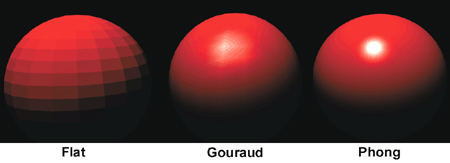
\includegraphics[width=0.99\linewidth]{images/gouroud-phong-flat.jpg}}
    \caption{A boat.}
\end{figure}

\todo[inline]{
    TODO: hablar sobre matriz de perspectiva de
    \href{http://www.cs.uns.edu.ar/cg/clasespdf/p465carlbom.pdf}
    {Ingrid Carlbon}
}

\todo[inline]{
    Siguientes a\~nos: antialising, sombras, multinucleo aparicion GPUs,
    raytracing...
    \href{https://ohiostate.pressbooks.pub/graphicshistory/back-matter/cg-historical-timeline/\#1970}
    {fuente}
}

\todo[inline]{
    Blinn’s law: “as technology advances, rendering time remains constant.” 
    from
    \href{http://www.pbr-book.org/3ed-2018/Introduction/A_Brief_History_of_Physically_Based_Rendering.html}
    {here}
}

\todo[inline]{
    Blinn's law: James Blinn first pointed out, in animation, rendering time remains
    constant, even as computers get faster. An artist gets accustomed to waiting a
    certain number of hours for an image to render, so as hardware improves, instead
    of using it to save time, he employs it to render more complex graphics. from
    \href{https://nevalalee.wordpress.com/2011/08/09/blinns-law-and-the-paradox-of-efficiency/}
    {here}
}

\todo[inline]{
    TODO: Esquema evolucion en el tiempo del shading: phong, blinn-phong
}


      \chapter{Marco colaborativo}
\todo[inline]{Cambiar/mejorar}
Seddi es una startup nacida como fruto de la investigacion en tecnologias de simulacion optica y mecanica aplicadas al sector textil.
Propone ofrecer una solucion digital que permita a los disenhadores, patronistas o comerciales trabajar en un entorno colaborativo que
representa con gran fidelidad los elementos constructivos de un prenda de ropa: tejido, costuras, dobladillos, etc.

La caida, el brillo y, en general, la apariencia de una prenda son factores clave para validar o rechazar el producto, estas caracteristicas
dependen de propiedades opticas y mecanicas que las herramientas de disenho actuales no tienen en cuenta, por lo que los profesionales del
sector no satisfacen las necesidades de los profesionales de la industria, que en la mayor parte de los casos mantienen un proceso de
trabajo artesanal en el que el prototipado y construccion de la prenda es un proceso iterativo entre patronista y disenhador y cuyo
resultado depende en gran medida de la experiencia y destreza de estos profesionales.\\

Para ofrecer su solucion, Seddi cuenta con departamentos de investigacion simulacion y captura tanto mecanica como optica, que desarrollan
nuevos algoritmos y hardware que permitan un mayor grado de fidelidad en el momento de captura de los parametros que conforman la apariencia
de una prenda, tanto como mejorar su representacion digital asi como departamentos de desarrollo de producto, se encargan del proceso de
captura utilizando estas tecnologias propietarias asi como de integrar estos algoritmos en diferentes plataformas que permitan al consumidor
final interactuar sobre los tejidos digitales durante diferentes etapas asociadas a este proceso de produccion con el fin de facilitar,
acelerar y reducir los costes de produccion.

Para conseguir un resultado fidedigno, en Seddi, el proceso comienza creando un clon digital del tejido, la obtencion de parametros opticos y
mecanicos que identifican el tejido y se valida utilizando las tecnologias de simulacion y render de la empresa. 

Todos las herramientas de Seddi se alojan en la nube, lo que garantiza disponibilidad inmediata a los recursos a todo el equipo involucrado en
el proceso de produccion. Estos equipos, con un negocio de la moda cada dia mas globalizado, pueden tratarse de equipos multidisciplinares de
diferentes empresas o paises, por lo que es primordial un flujo de comunicacion constante que minimice los errores y los costes economicos y
medioambientales de los flujos de disenho y prototipado

Gracias a esta estrategia de implementación, el contenido diseñado está disponible de manera inmediata y editable en un escenario global. En la
actualidad, el negocio de la moda está completamente globalizado, y las tareas de diseño y prototipado de muchas marcas se hacen entre equipos
internacionales o mediante subcontratación entre empresas. La  utilización de las soluciones cloud de Seddi permitirá a los equipos colaborar remotamente sobre un mismo diseño.
En Seddi, el proceso para llegar a construir una prenda, comienza con la digitalizacion de un tejido, que se consigue a partir de muestras que
son analizadas por maquinas de captura desarrolladas en Seddi, para obtener los parametros mecanicos y opticos

      \chapter{Estado del arte}
      \chapter{PBR}
PBR o \textit{physically based rendering} es el t\'ermino que se utiliza para nombrar al grupo de t\'ecnicas basados en un
modelo f\'isico. La intenci\'on de los sistemas de renderizado PBR en entornos interactivos es conseguir aproximaciones plausibles
y poco costosas de la dispersi\'on de la luz al golpear sobre una superficie. Las principales ventajas de este tipo de algoritmos
son la consistencia bajo diferentes condiciones de luz y su manejo intuitivo por parte de los artistas.\\

% Los motores PBR cumplen con la ley de la conservaci\'on de la energ\'ia y utilizan BRDFs basados en la teor\'ia de
% microfacetas y el principio de reciprocidad de Helmholtz

Aunque este trabajo se centra en el tratamiento de materiales basados en aspectos f\'isicos, adicionalmente, otros elementos
de la escena, como la c\'amara o las luces, pueden estar basados en modelos f\'isicos para ofrecer un mayor grado de realismo.

\section{Unidades radiom\'etricas}
    % \todo[inline]{
    %     When we talk about light arriving (or leaving) a surface from a certain direction, it’s
    %     more appropriate to speak in terms of the quantity of light arriving at or passing through a
    %     certain area of space. The reason for this is that light is measured in terms of flow
    %     through an area. That is, light is measured as energy per-unit surface area (i.e.
    %     Watts/meter2). This means it doesn’t really make sense to talk about the amount light
    %     arriving from a single incoming direction – it’s more appropriate to talk about light
    %     coming from a small region of directions.
    % }
    % \todo[inline]{
    %     Since BRDFs measure how light reflects off a surface when viewed under various
    %     viewing positions, we must have a good understanding of how much light arrives at a
    %     surface element (or leaves a surface element) from a particular direction.
    % }
    Los modelos de BRDF analizados en este trabajo son basados en f\'isica y utilizan las unidades radiom\'etricas para
    medir las interacciones f\'isicas de la luz con el entorno. A continuaci\'on un listado de las unidades
    b\'asicas de radiometr\'ia:
    % para describir la luz incidente sobre las superficies.

    \subsection*{\'Angulo s\'olido}
    El \'angulo s\'olido ($w$) es la unidad de medida del \'area de una proyecci\'on sobre una esfera de radio 1  es el
    equivalente tridimensional a la medida en radianes de un arco sobre un c\'irculo. Su unidad es el est\'ereorradi\'an
    ($sr$), que representa el \'area de un \'angulo s\'olido sobre la esfera de radio unitario $\Omega$ que contiene $4\pi$ radianes.

    \begin{figure}[H]
        \vspace{0.5cm}
        \centering
          \frame{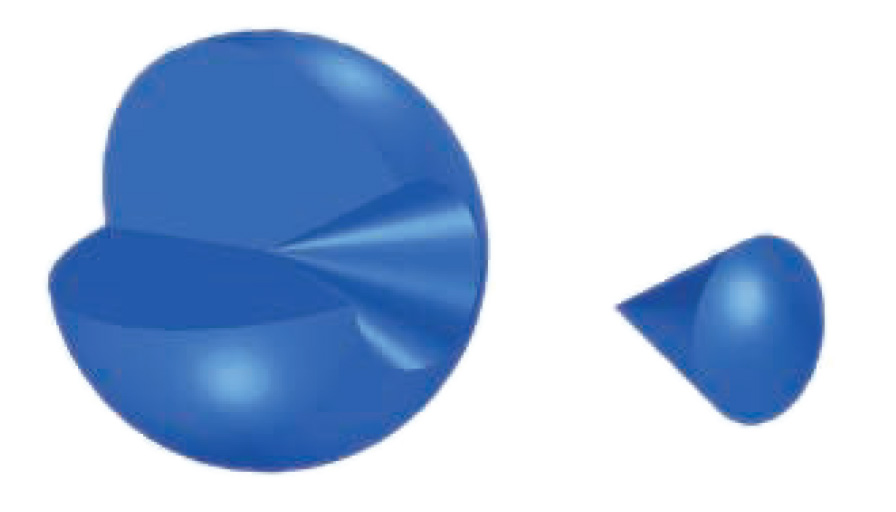
\includegraphics[scale=0.42]{steradian}}
        \caption{La superficie de la base del cono extra\'ido de la esfera representa 1$sr$.}
        \vspace{0.5cm}
    \end{figure}

    \subsection*{\'Angulo s\'olido diferencial}
    Es la unidad que se utiliza como \'area de medida en el BRDF para representar la cantidad de luz que incide en una superficie.
    Un \'angulo s\'olido diferencial ($dw$) es el \'area contenida entre incrementos muy peque\~nos en coordernadas esf\'ericas sobre
    los \'angulos $\theta$ y $\phi$ de la semiesfera $\Omega$.

    \begin{figure}[H]
        \vspace{0.5cm}
        \centering
          \frame{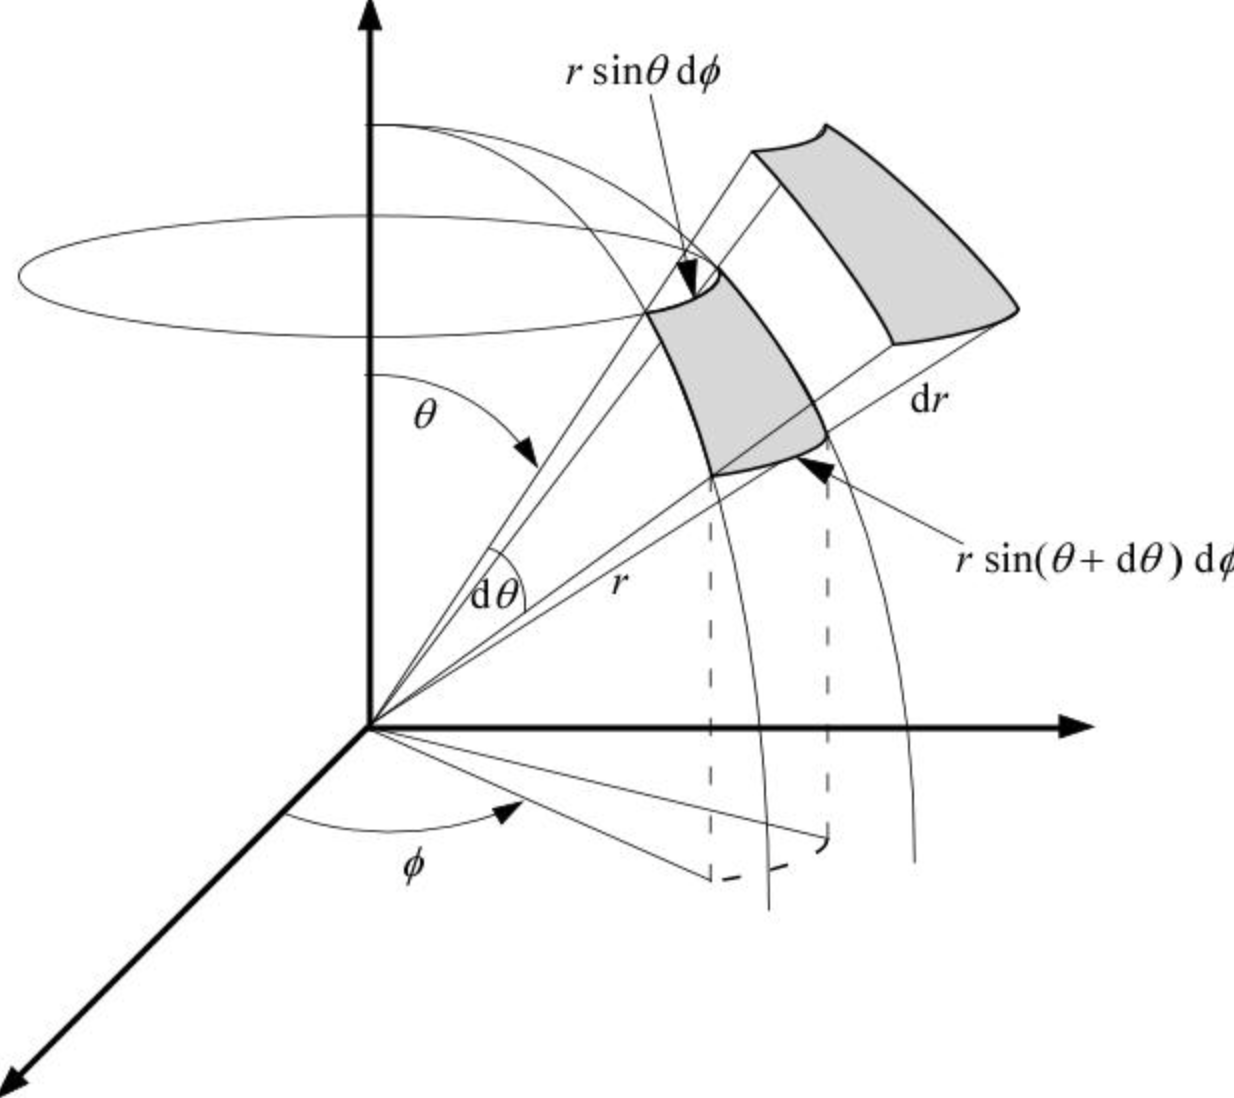
\includegraphics[scale=0.24]{differentialsolidangle}}
        \caption{Esquema explicativo de un \'angulo s\'olido diferencial.}
        \vspace{0.5cm}
    \end{figure}

    % \todo[inline]{
    %     Since both the width and the height of the rectangular patch are measured in radians, the
    %     area quantity has units of radians squared (or steradians). Steradians sounds like a fancy
    %     word, but really it’s not too bad. If ever you find the term confusing, just think of it as
    %     “solid angle units” or “radians squared”. The abbreviation for steradians is sr.
    % }

    \subsection*{Flujo radiante}
        El flujo radiante ($\Phi$) es la unidad que mide la  cantidad de energia de energ\'ia transportada
        por las ondas de luz por unidad de tiempo. En los motores de renderizado utilizan esta unidad para expresar la cantidad
        total de energia emitida por una fuente de luz y se mide en vatios ($W$).
        % \begin{equation}
        %     \Phi_e = \dfrac{d{Q_e}}{dt}
        % \end{equation}

    \subsection*{Irradiancia}
        La irradiancia ($E$) es la cantidad de energ\'ia (flujo radiante) de tiempo por unidad de superficie y
        se mide en vatios por metro cuadrado ($W/m^2$). En los motores de render se utiliza
        para medir la cantidad de luz que incide sobre un punto desde todas las direcciones.

        \begin{equation}
            E = \dfrac{d\Phi}{dA}
        \end{equation}

        \begin{figure}[H]
            \vspace{0.5cm}
            \centering
              \frame{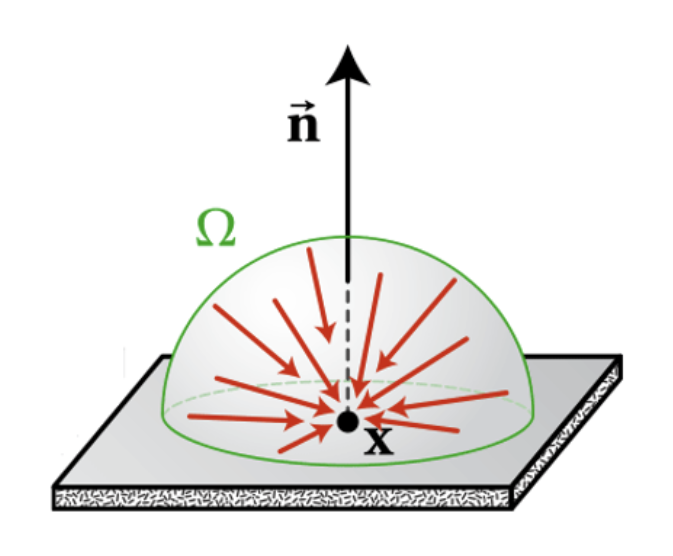
\includegraphics[scale=0.44]{irradiance}}
            \caption{La superficie de la base del cono extra\'ido de la esfera representa 1$sr$.}
        \end{figure}


    \subsection*{Intensidad radiante}
        Representa el flujo radiante emitido por una fuente de luz en una direcci\'on determinada y se mide expresa
        como vatios por estereorradi\'an ($W/sr$).

        \begin{equation}
            I = \dfrac{d\Phi}{d\omega}
        \end{equation}

    \subsection*{Radiancia}
        La radiancia ($L$) se puede considerar como la combinaci\'on de irradiancia e intensidad radiante y
        define la direcci\'on y la intensidad radiante recibida por una superficie. La ecuaci\'on de render, igual que la c\'amaras,
        sensores o nuestros ojos miden la radiancia que llega desde las superficies del entorno al punto de vista. Su unidad son los
        vatios por metro cuadrado por estereorradi\'an (${W}/{m^2sr}$)
        \begin{equation}
            L = \dfrac{d^2\Phi}{dA_{proj}d\omega}
        \end{equation}

        \begin{figure}[H]
            \vspace{0.5cm}
            \centering
              \frame{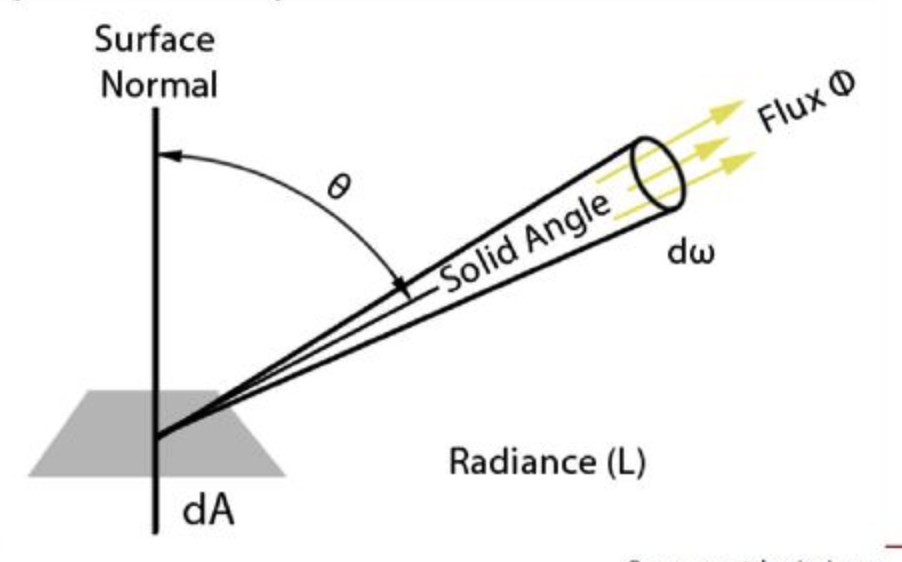
\includegraphics[scale=0.4]{radiance}}
            \caption{La superficie de la base del cono extra\'ido de la esfera representa 1$sr$.}
            \vspace{0.5cm}
        \end{figure}

\section{Ecuaci\'on de render}
Presentada por primera vez en el trabajo de Jim Kajiya \autocite{kajiya}, el prop\'osito de la ecuacion de render es conocer el valor de
radiancia que llega a la camara en una direcci\'on por cada pixel de la camara. Para ello se utiliza la ecuacion de reflectancia,
que depende de la luz que llega al punto, el coseno del angulo con el que incide la luz y el BRDF, que modela el comportamiento
de la luz al rebotar sobre la superficie.\\

\begin{eqfloat}[!htb]
    \begin{equation}
        L_o(p, w_o) = L_e(x, w_o) + \int_\Omega{f_r(p, w_i, w_o) L_i(p, w_i) n\cdot{w_i}dw_i}
    \end{equation}
  \caption{Ecuaci\'on de render}
\end{eqfloat}
\singlespacing

Siendo $L_o(p, w_o)$ la luz reflectada por la superficie, $L_e(x, w_o)$ la luz emitida por la superficie, que est\'a fuera
de la integral porque es independiente de la luz reflejada por la superficie. $\int_{\Omega}[...]dw$ que representa
que la operaci\'on se repite para cada \'angulo s\'olido dentro de la semiesfera $f_r(p, w_i, w_o)$, el BRDF, $L_i(p, w_i)$, la luz
que llega al punto de la superficie que estamos evaluando y $n\cdot{w_i}$ el factor de atenuaci\'on de la luz con respecto a la normal.\\

\begin{figure}[H]
    \vspace{0.5cm}
    \centering
    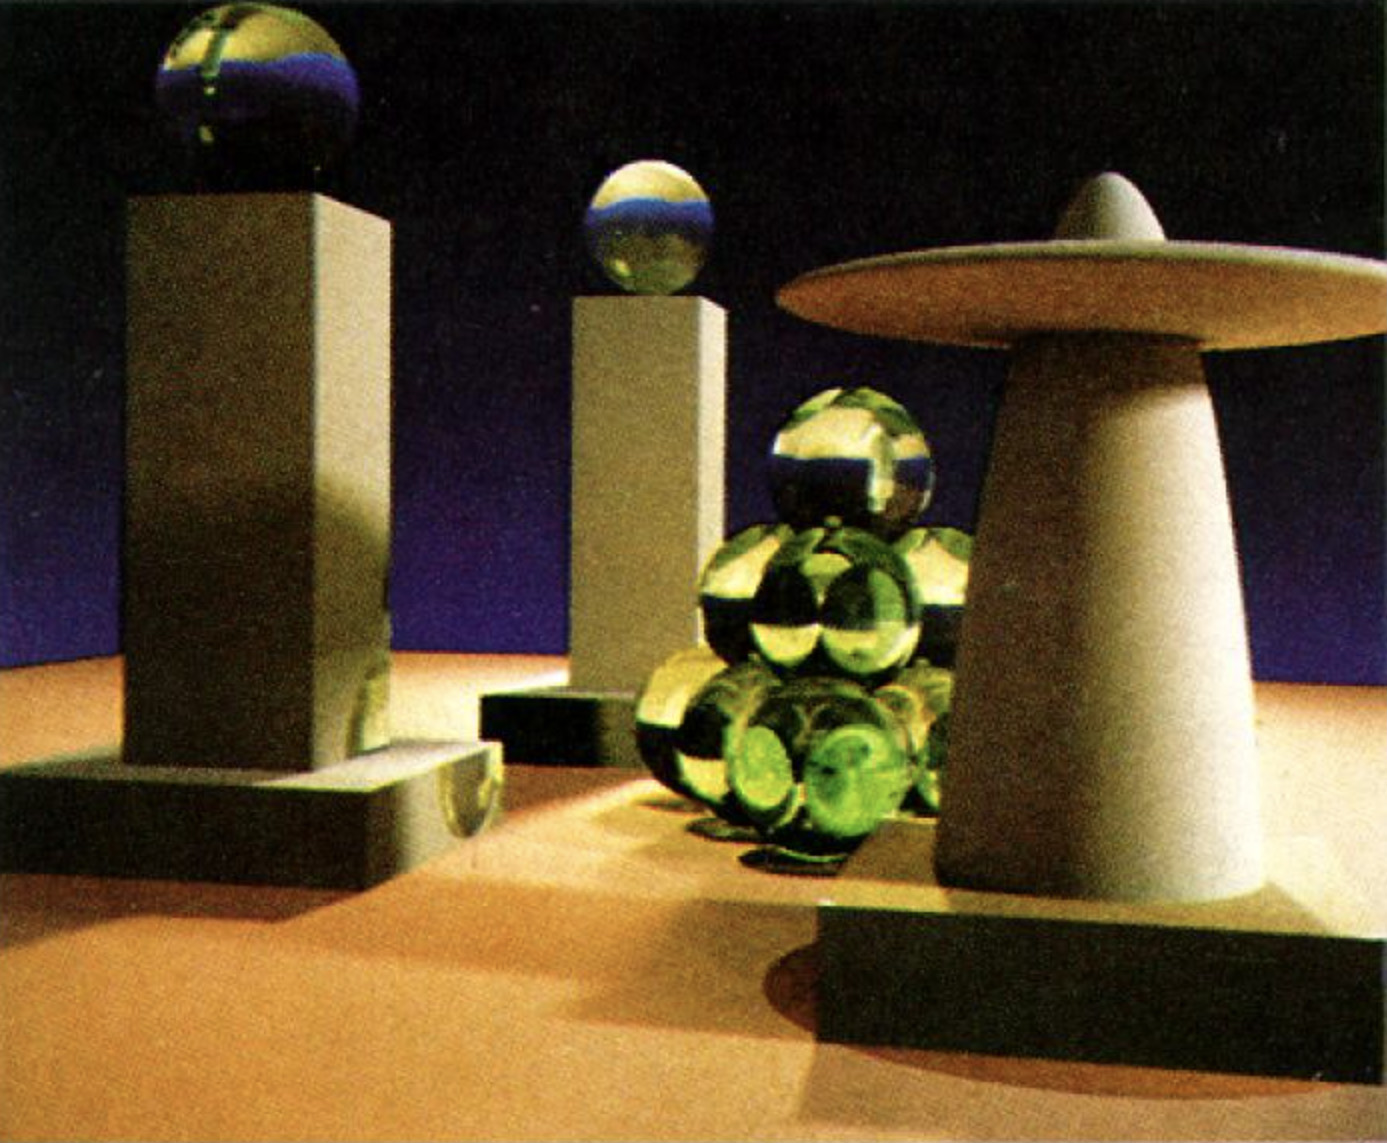
\includegraphics[scale=0.35]{renderequation}
    \caption{Im\'agen publicada originalmente en el trabajo de Kajiya \autocite{kajiya}}
    \vspace{0.5cm}
\end{figure}

El coste de computaci\'on de la radiancia debida al conjunto del entorno (iluminaci\'on indirecta o global) es muy alto, por lo que
tradicioanlmente los sistemas de renderizado interactivos calculaban \'unicamente la radiancia debida a los emisores de luz de la escena
(iluminaci\'on directa o local). Sin embargo recientemente se han presentado t\'ecnicas que permiten la aproximaci\'on
de este efecto que se analizan en la \'ultima secci\'on de este cap\'itulo.

% \todo[inline]{
%     An important property of the rendering equation is that it is linear with respect to
%     the emitted lighting. If we make the lights twice as strong, the result of the shading will
%     be two times brighter. The response of the material for each light is also independent
%     from other sources. That is, one light’s presence does not affect the interaction of
%     another light with the material.\\
% }

% \todo[inline]{
%     In real-time rendering, it is common to use just a local lighting model. Only the
%     surface data at visible points are needed to compute the lighting—and that is exactly
%     what GPUs can most efficiently provide.\\
% }

\section{BRDF}

El BRDF, o función de ditribuci\'on bidireccional de reflectividad, es la parte de la ecuaci\'on $f_r(p, w_i, w_o)$ que describe el
comportamiento de la luz al golpear sobre la superficie y se utiliza para modelar propiedades f\'isicas de los diferentes
materiales.\\

Es una funcion estad\'istica que calcula el ratio de luz que incidente sobre un material que es reflejada en direcci\'on
a la c\'amara, para ello toma como argumentos la direccion de la luz, $w_i$, y la dirección de la vista,
$w_o$, la normal de la superficie, $n$, y un par\'ametro $\alpha$ que representa la rugosidad del material.

\begin{figure}[H]
    \vspace{0.5cm}
    \centering
      \frame{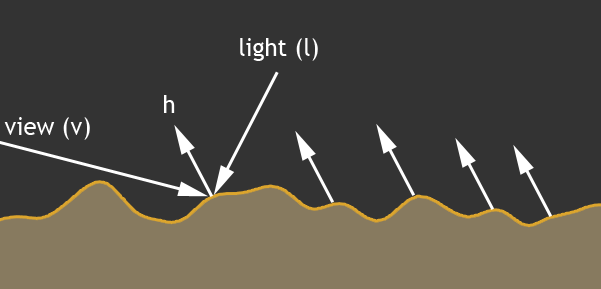
\includegraphics[scale=0.5]{microfacet-diagram}}
    \caption{Diagrama de la luz incidente y luz reflectada}
    \vspace{0.5cm}
\end{figure}

% \todo[inline]{
%     Las caracter\'isticas esenciales de un motor PBR, adem\'as de estar basado en la teor\'ia de microfacetas, son cumplir con el principio
%     de conservaci\'on de la energ\'ia y el principio de Helmholtz. Estos dos principios no siempre se cumplen en los sistemas de
%     de renderizado realista en entornos interactivos, que pueden presentar optimizaciones que sacrifiquen aspectos f\'isicos del modelo
%     en favor de tiempos de respuestas menores, siempre y cuando no resulten en artefactos apreciables.\\
% }

Los BRDFs basados en aspectos f\'isicos, adem\'as de estar basados en la teor\'ia de microfacetas, se caracterizan por otras dos
propiedades: el principio de reciprocidad de Helmholtz y la ley de conservaci\'on de la energ\'ia.

% \todo[inline]{
%     Para que un BRDF se considere como PBR, ha de utilizar el modelo de microfacetas, ademas de cumplir con la ley de conservacion
%     de la energia,  y el principio de reciprocidad de Helmholtz,
%     el BRDF debe de ser simétrico, esto es que invertir la direccion de entrada y salida del BRDF no deberia afectar al resultado
%     $f(x, w_i, w_o) = f(x, w_o, w_i)$ sin embargo, los motores en tiempo real, frecuentemente incumplen el principio de reciprocidad,
%     no siendo fisicamente plausibles, pero sin generar artefactos.\\
% }
\begin{itemize}
    \item
        El principio de reciprocidad de Helmholtz establece que el BRDF debe de ser simétrico, lo que supone que invertir las direcciones
        de entrada y salida del BRDF no debe afectar al resultado.
        
        \begin{equation}
            f(x, w_i, w_o) = f(x, w_o, w_i)
        \end{equation}
        \singlespacing

        \item El principio de conservaci\'on de la energ\'ia determina que la energ\'ia dispersada por la superficie no puede
    ser mayor que la energ\'ia incidente.

    \begin{equation}
        \forall w_i \int_{\Omega} f(p, w_i, w_o) n\cdot{w_i} dw_o \leq 1
    \end{equation}
\end{itemize}
\singlespacing

Estos dos principios no siempre se cumplen en los sistemas de de renderizado realista en entornos interactivos, que pueden presentar
aproximaciones que sacrifiquen aspectos f\'isicos del modelo, siempre y cuando no resulten en artefactos visuales apreciables, en
favor de tiempos de respuestas menores.

    \subsection{Teor\'ia de microfacetas}

    \bgroup

        Aunque a escala macrosc\'opica podamos considerar una superficie como lisa, ninguna superficie es completamente lisa a nivel
        microsc\'opico. La teor\'ia de microfacetas utiliza una representaci\'on estad\'istica para modelar estas peque\~nas irregularidades.\\

        La teor\'ia de microfacetas, considera la superficie de reflexi\'on como una superficie compuesta por una matriz de
        superficies mas peque\~nas que la longitud de onda de la luz, completamente reflectantes, llamadas microfacetas, y cuyas
        diferentes orientaciones determinan la rugosidad de la superficie.\\

        \begin{figure}[H]
            \centering
            \frame{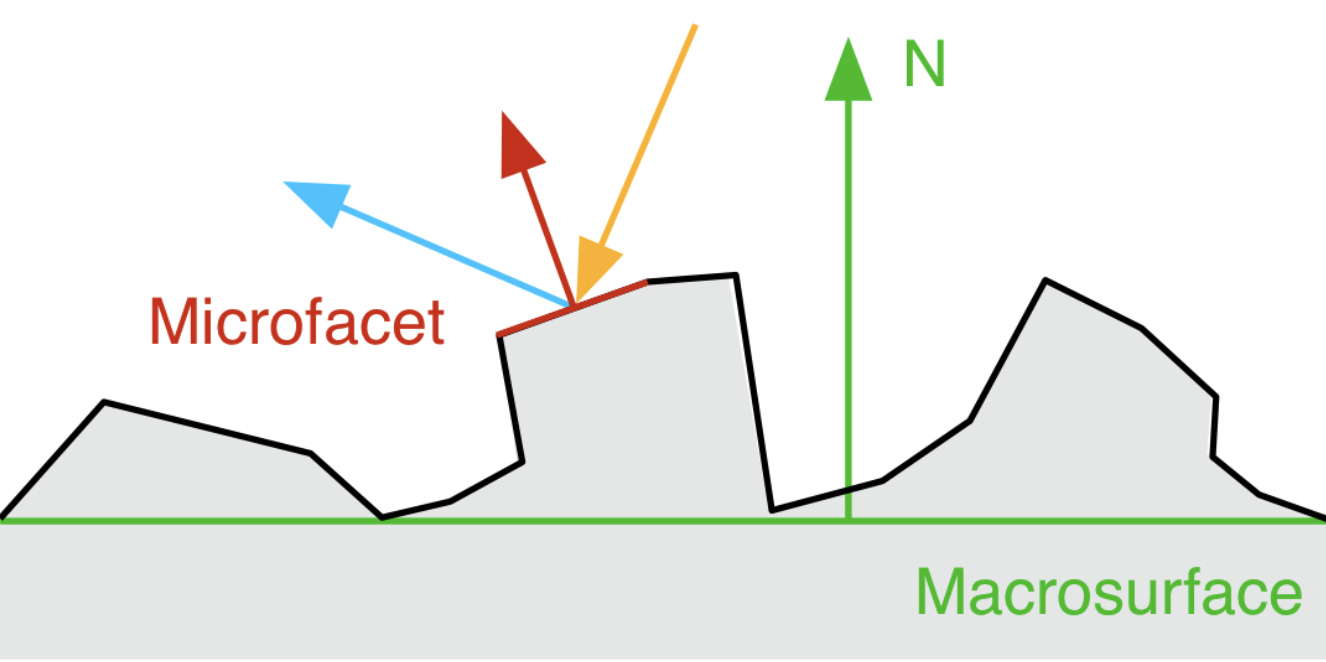
\includegraphics[scale=0.55]{macrosuperficie}}
            \caption{Superficie a escala microsc\'opica}
            \vspace{0.5cm}
        \end{figure}

        Si las normales de las microfacetas est\'an completamente alineadas con el vector medio entre la vista y la luz (vector $h$),
        las reflexiones ser\'an mas definidas, asimilandose a un espejo, mientras la variaci\'on de la normal de las microfacetas con
        respecto al vector $h$ dar\'a como resultado una reflexion especular mas difusa.

    \egroup


    \subsection{Tipos de BRDFs}
    Existen diferentes tipos de BRDFs en funci\'on de las propiedades f\'isicas del material que se quiera representar. Los
    materiales met\'alicos utilizan un BRDF diferente a los diel\'ectricos, esto es as\'i porque los efectos de absorci\'on y
    dispersi\'on, son completamente diferentes en funci\'on de esta propiedad.\\

    En los materiales metalicos, la reflexi\'on especular es de color, la luz refractada es absorbida por el propio material
    y no existen efectos de dispersi\'on de la luz bajo la superficie, mientras que en los materiales diel\'ectricos, o no
    met\'alicos, el aspecto final del material esta determinado por una combinaci\'on de los fen\'omenos de absorci\'on y
    dispersi\'on de la luz.\\

    Por otra parte, podemos diferenciar entre materiales anisotr\'opicos, como el metal pulido o el pelo, cuyas propiedades
    de reflexi\'on cambian al rotar sobre la superficie alrededor de su vector normal. Aunque casi todos los materiales son, en cierta medida, anisotr\'opicos, la
    aportaci\'on de esta propiedad sobre la apariencia final suele ser tan baja que se desprecia y se utilizan modelos
    isotr\'opicos.\\

    Adem\'as, seg\'un su origen, podemos distinguir principalmente entre tres tipos de modelos: emp\'iricos, te\'oricos y
    experimentales. Los modelos emp\'iricos no est\'an basados en f\'isica, si no que son simplificaciones de menor coste que
    aproximan un determinado fen\'omeno, ejemplos de modelos emp\'iricos son los modelos de Phong \autocite{phong} o el
    de Blinn-Phong \autocite{blinnphong}. Los modelos te\'oricos, como los basados en microfacetas, se basan en observaciones sobre el comportamiento de la luz y su
    interacci\'on sobre las superficies para crear un sistema de ecuaciones que describan este comportamiento sobre un modelo
    matem\'atico. Por \'ultimo, los modelo experimentales, el de Schlick \autocite{schlick} se basan en resultados obtenidos en estudios de campo con luz a partir de los
    cuales se crean funciones que se ajusten a los datos obtenidos.
    % Los diferentes tipos de BRDFs permiten para modelar diferentes propiedades de los materiales, isotropia o anisotropia,
    % transmitancia, reflexiones internas, etc. Podemos clasificar los diferentes tipos de BRDFs entre modelos analiticos y BDRFs
    % de datos adquiridos. Los modelos analiticos son funciones matemáticas que modelan diferentes efectos de la luz en funcion de
    % sus datos de entrada, mientras que los BRDFs de datos adquiridos, capturan el BRDF de un material con un gonioreflectometro,
    % y permiten una representacion muy precisa del material escaneado.

    % Comunmente, en la industria se utilizan modelos anal\'iticos, debido a su flexibilidad y rendimiento y el mas utilizado a
    % d\'ia de hoy en la industria, aunque con algunas variaciones en sus t\'erminos, sigue siendo el modelo de Cook-Torrance\autocite{cooktorrance}.
    % \todo[inline]{
    %     Metal. The appearance of the metal mainly depends on the direct reflection of light at the interface of the two media (ie, specular reflection). The metallic specular reflection color is a three-channel color, and R, G, and B are different. The light refracted into the metal is almost immediately absorbed by free electrons, and there is no scattering of light refracted into the metal.
    %     Non-Metal. Non-metal is a dielectric, and its overall appearance is mainly determined by its combination of absorption and scattering characteristics. Similarly, the interaction between non-metal and light is divided into reflection and refraction. According to the scattering and absorption characteristics of the medium type, refraction is divided into multiple categories:
    % }
    % \todo[inline]{
    %     The term isotropic is used to describe BRDFs that represent reflectance properties that
    %     are invariant with respect to rotation of the surface around the surface normal vector.
    %     Consider a small relatively smooth surface element and fix the light and viewer positions.
    %     Anisotropy, on the other hand, refers to BRDFs that describe reflectance properties that
    %     do exhibit change with respect to rotation of the surface around the surface normal
    %     vector. Some examples of materials that have anisotropic BRDFs are brushed metal,
    %     satin, and hair.
    % }

    \begin{figure}[H]
        \vspace{0.5cm}
        \centering
        \frame{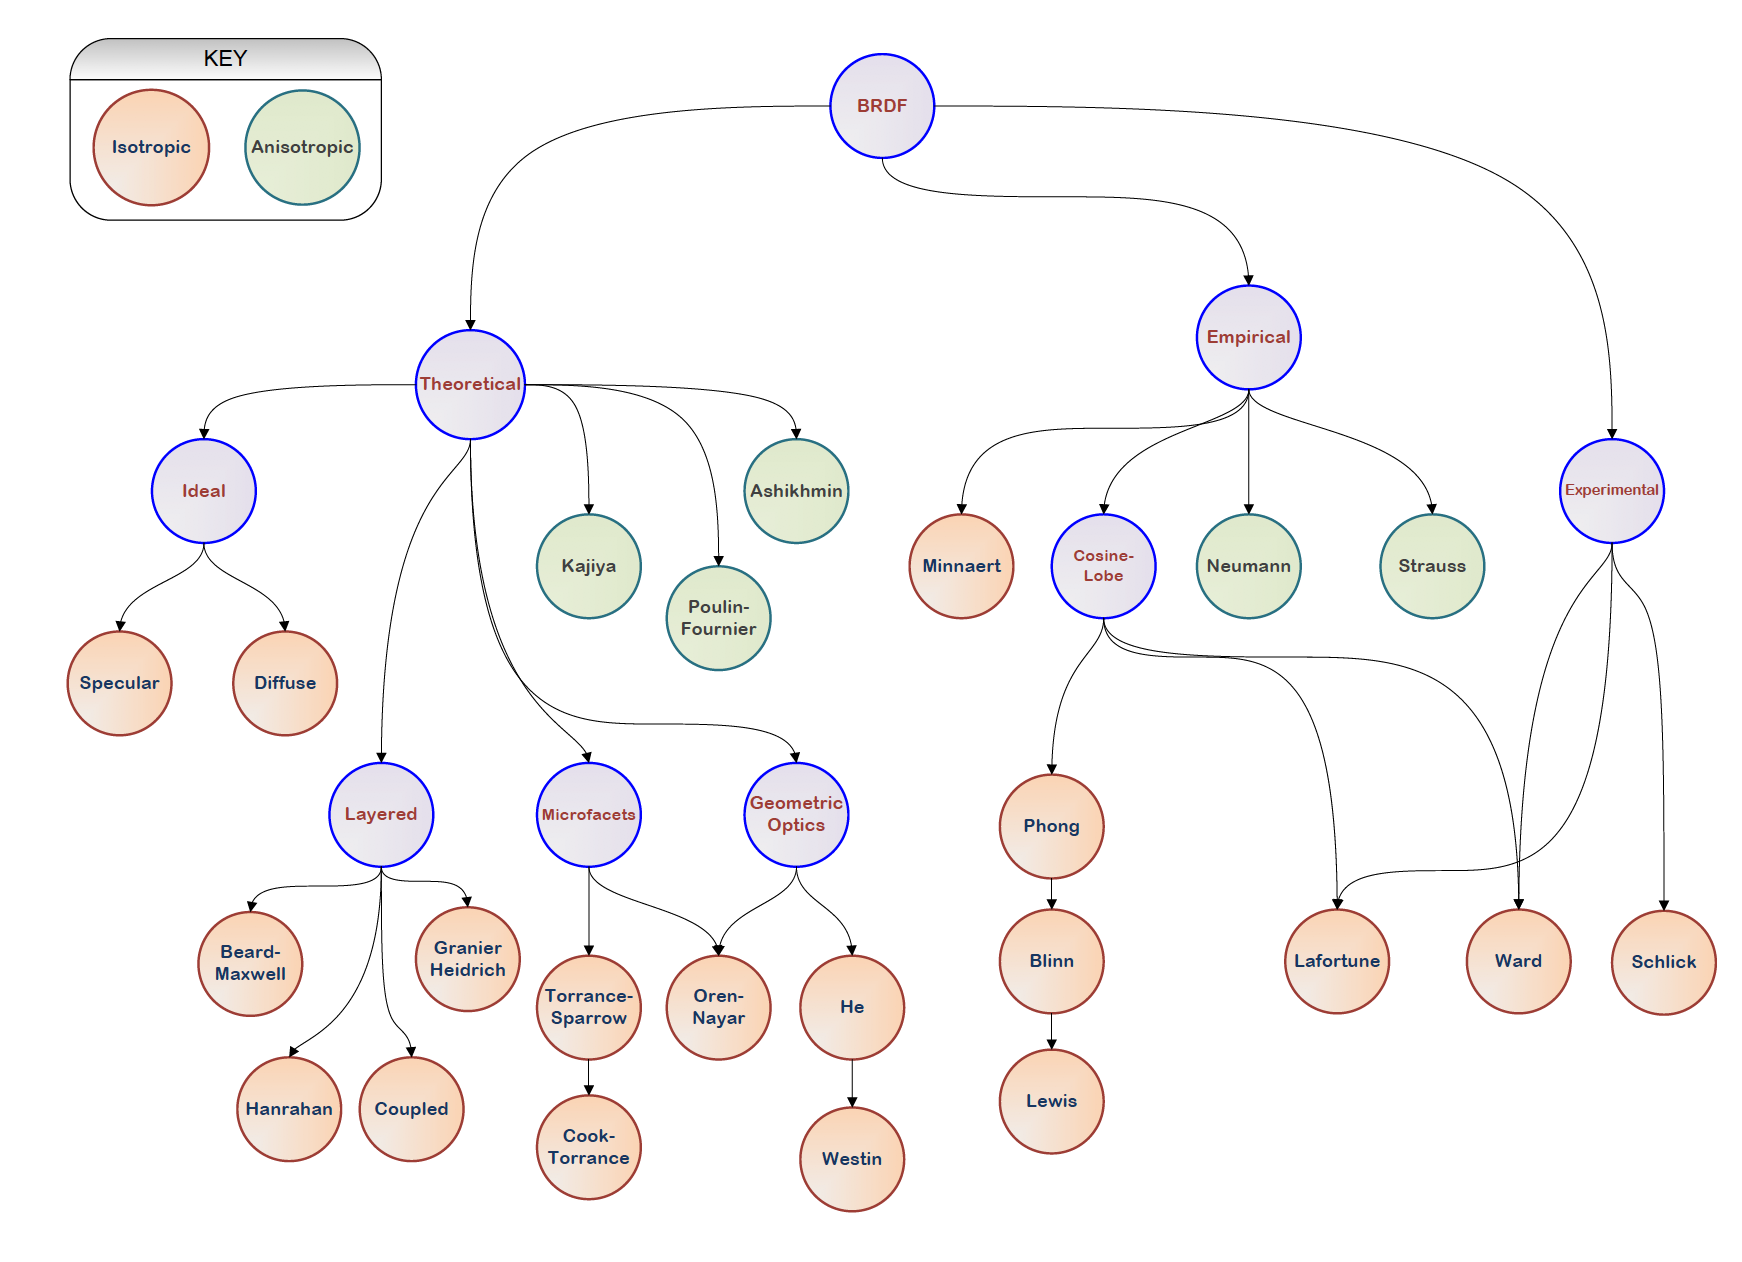
\includegraphics[scale=0.45]{schema_brdfs}}
        \caption{Esquema de diferentes modelos de BRDF seg\'un su origen}
        \vspace{0.5cm}
    \end{figure}

    \section{Modelo de Cook-Torrance}
    El modelo de BRDF de Cook-Torrance \autocite{cooktorrance} presenta la forma que conocemos a d\'ia de hoy: los t\'erminos
    de distribuci\'on de las normales, geometr\'ia y Fresnel y el factor de correcci\'on en el denominador. Aunque con cambios en
    sus t\'erminos, ideas pcomo la conservaci\'on de la energ\'ia, que solo las microfacetas cuyas normales apuntan en
    direcci\'on $h$ contribuyen a la reflexi\'on especular o la diferencia entre materiales met\'alicos y diel\'ectricos siguen
    presentes en la mayor\'ia de modelos basados en aspectos f\'isicos que se utilizan en la actualidad.

    \singlespacing
    $$
    f_r = k_{d}f_{lambert} + k_sf_{cook-torrance}
    $$
    \begin{eqfloat}[!htb]
        \begin{equation}
            \textrm{siendo}\ k_d + k_s = 1
        \end{equation}
        \caption{Ley de conservaci\'on de la energ\'ia en el modelo de Cook-Torrance \autocite{cooktorrance}}
    \end{eqfloat}
    
    Este trabajo populariz\'o los modelos basados en aspectos f\'isicos al permitir representar con gran realismo materiales
    el\'ectricos y diel\'ectricos con diferentes niveles de rugosidad. Su principal desventaja es su parametrizaci\'on, que
    no resulta intuitiva y dificulta el trabajo de los artistas de 3D.

    \begin{figure}[H]
        \centering
        \frame{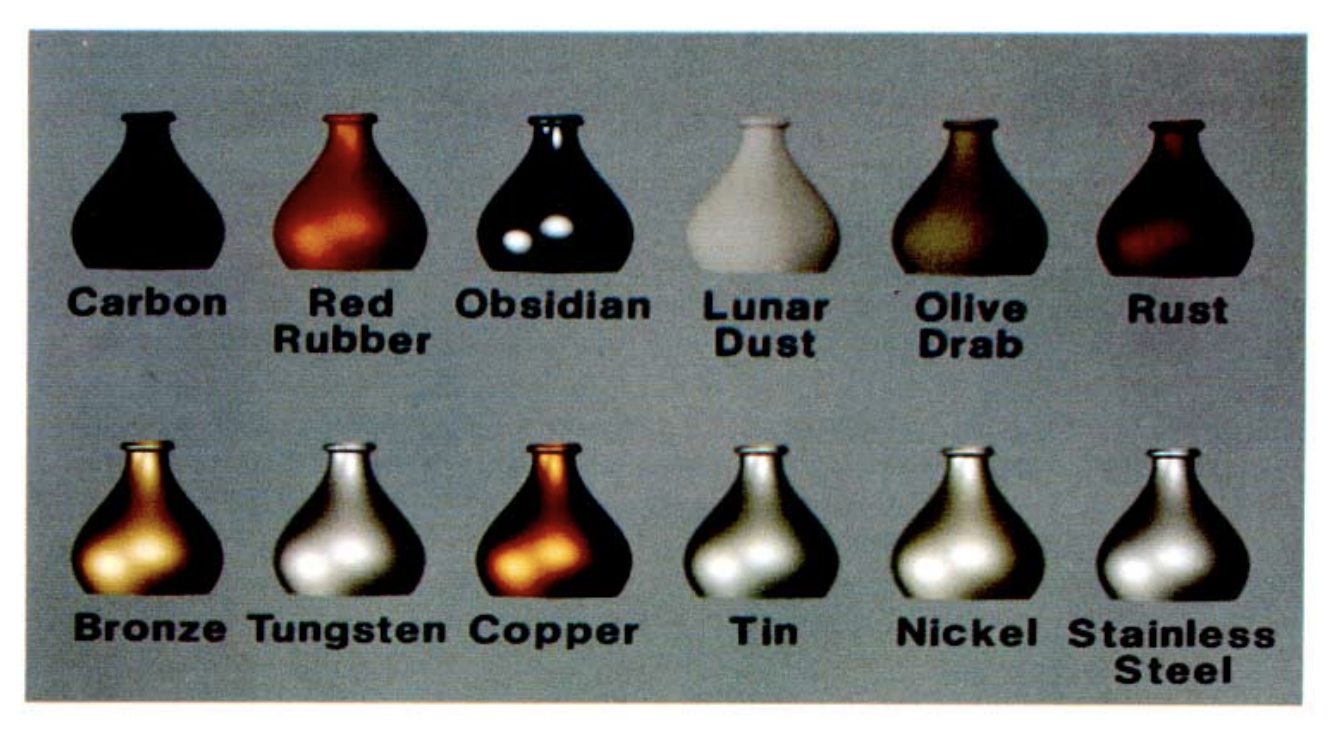
\includegraphics[scale=0.45]{cooktorrance}}
        \caption{Diferentes tipos de materiales representados por el modelo de Cook-Torrance \autocite{cooktorrance}}
    \end{figure}

    % Este modelo presenta por primera vez el concepto de conservaci\'on de la energ\'ia, que se aplica sobre las
    % componentes especular y difusa:
    
    % \begin{figure}[H]
    %     \centering
    %     \frame{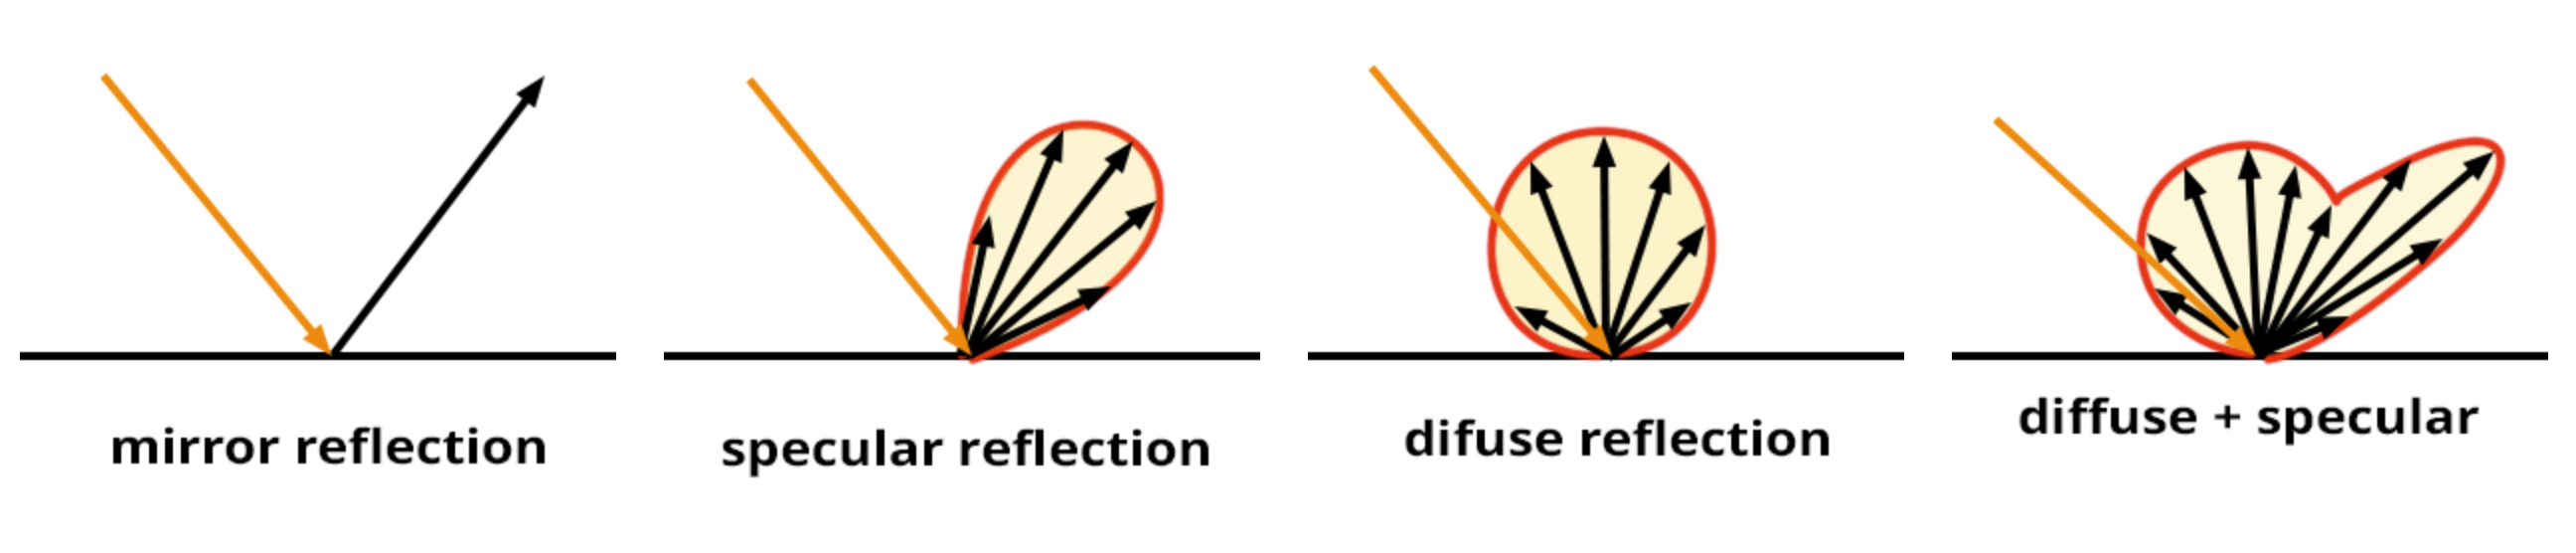
\includegraphics[scale=0.32]{diffusespecular}}
    %     \caption{Tipos de reflexi\'on}
    %     \vspace{0.5cm}
    % \end{figure}

        \subsection{Componente difusa}
        T\'ipicamente la componente difusa, utiliza el modelo de Lambert, que asume una distribuci\'on completamente uniforme a lo
        largo de la superficie:\\
        
        \begin{equation}
        f_{Lambert} = \frac{diffuse}{\pi}
        \end{equation}
        \singlespacing
    
        \subsection{Componente especular}
            La componente especular es una funci\'on compuesta de otras tres t\'ermino y un factor de normalizaci\'on en el
            denominador.\\

            \begin{equation}
                f(l, v) = \frac{F(w_i, h) G(w_i, h, w_o) D(h)} {4(n\cdot{w_i}) (n \cdot{w_o})}
            \end{equation}
            \singlespacing
            
            
            El denominador es una caracter\'istica t\'ipica de los modelos de microfacetas y es un factor de correci\'on
            debido al cambio de espacio entre el espacio local de las microfacetas y el espacio local de la macrosuperficie. Para modelos
            que no incluyen este factor, se puede aplicar un factor de sombreado directamente multiplicando el t\'ermino de geometr\'ia
            por el factor $\frac{1}{4(n\cdot{w_i}) (n\cdot{w_o})}$.\\

            \singlespacing
            \subsection*{D, t\'ermino de distribuci\'on de las normales}
            Es la funci\'on de distribuci\'on de las normales y es un modelo estad\'istico que se encarga de representar
            la rugosidad de una superficie y es el t\'ermino que afecta en mayor grado a la forma y taman\~no del brillo especular. T\'ipicamente el par\'ametro de
            rugosidad se utiliza para representar la cantidad de microfacetas alineadas con la normal $h$, cuanta mayor sea la
            la cantidad de de microfacetas alineadas, m\'as lisa parecer\'a la superficie.\\

            \begin{figure}[H]
                \vspace{0.5cm}
                \centering
                \frame{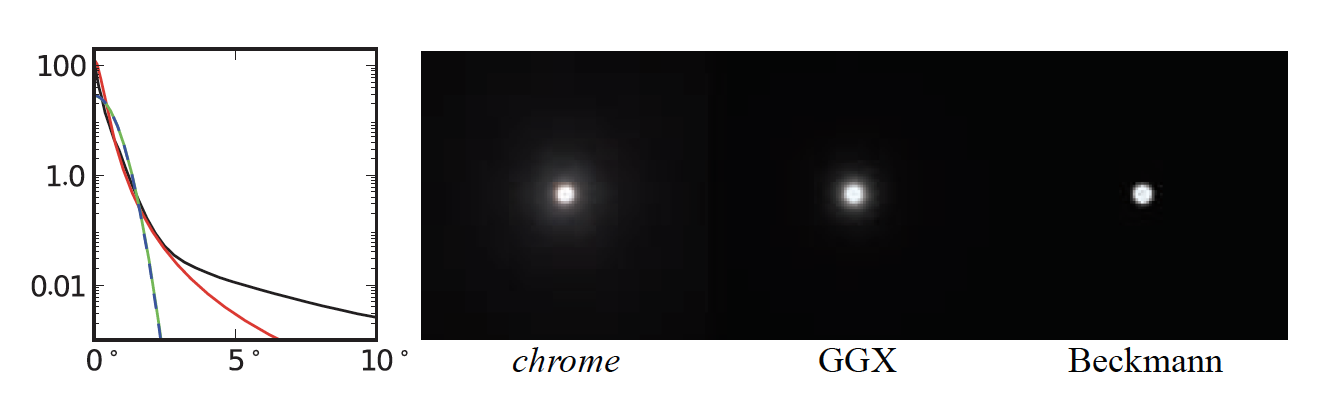
\includegraphics[scale=0.65]{ndf}}
                \caption{Modelos de distribuci\'on de microfacetas frente a la muestra de referencia}
                \vspace{0.5cm}
            \end{figure}

            La funci\'on de distribuci\'on de microfacetas utiizada por este modelo es la presentada por Beckmann \autocite{beckmann}:\\

            \begin{equation}
                D(h) =
                \frac{1}{\pi\alpha^2(n\cdot{h})^4}
                e^{
                    \frac
                    {(n\cdot{h})^2 - 1}
                    {m^2(n\cdot{h})^2}
                }
            \end{equation}
            \singlespacing

            \subsection*{F, t\'ermino de Fresnel}
            Representa la radiancia reflejada por un material seg\'un el \'angulo de incidencia
            de la luz. Para la mayor\'ia de los materiales no met\'alicos, las reflexiones son m\'as intensas bajo cuando el \'angulo
            de incidencia es muy agudo.\\

            En la f\'ormula original de Fresnel, la energ\'ia depende del \'indice de refracci\'on $\eta$ y el \'indice de refracci\'on
            $\kappa$, coeficientes no siempre conocidos para un material. La aproximaci\'on a la funci\'on de Fresnel, otra de las
            principales contribuciones de este modelo, elimina $\kappa$ de la parametrizaci\'on.
            % \todo[inline]{
            %     One of the major contributions of this work [CT82] was
            %     the development of an optimized formulation of Fresnel,
            %     making this model more applicable to Computer Graphics.
            %     In the original formulation, the energy reflected depends on
            %     the index of refraction $\eta$, and the absorption coefficient $\kappa$
            % }

            $$
            F(\theta) = 
            \frac{1}{2}
            \frac{(b - c)^2}{(b + c)^2}\
            \bigg\{
                1 +
                \frac{[ \ c(b + c) - 1 \ ]^2}{[ \ c(b - c) + 1 \ ]^2}
            \bigg\}
            $$

            \begin{equation}
                \textrm{siendo} \; b^2 = \eta^2 + c^2 - 1 \; y \; c = cos(\theta)
            \end{equation}
    
            \begin{figure}[H]
                \vspace{0.5cm}
                \centering
                \frame{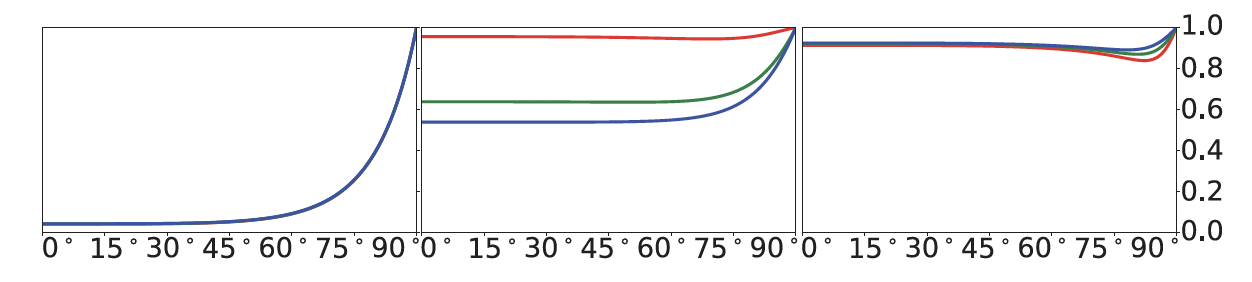
\includegraphics[scale=0.65]{fresnel}}
                \caption{Representaci\'on gr\'afica de la funci\'on de Fresnel}
                \vspace{0.5cm}
            \end{figure}
            \singlespacing

    
            \subsection*{G, t\'ermino de geometr\'ia}
            Para estimar la cantidad de microfacetas que contribuyen a la reflexi\'on especular, adem\'as de tener en cuenta
            la densidad de microfacetas cuyas normales est\'an orientadas en direcci\'on a $h$, se ha de calcular teniendo en
            cuenta la cantidad de rebotes ocluidos por las propias microfacetas. Este trabajo utiliza para ello el t\'ermino
            presentado en el modelo de Torrance-Sparrow \autocite{torrancesparrow}.\\

            % Mientras que la funci\'on de distribuci\'on de , la funci\'on de geometr\'ia 
            % Esta funci\'on tiene en cuenta las oclusiones debidas a la propia superficie.
            % Mientras que el t\'ermino de distribucion de las normales, $D(h)$, define la concentraci\'on de microfacetas con la normal
            % a la microfaceta ($h$), no define si esas microfacetas son visible o no.
            % \todo[inline]{
            %     El t\'ermino de geometr\'ia tiene en cuenta las dos cosas, la sombra
            %     y el enmascaramiento. La sombra representa que una microfaceta no es visible desde la direcci\'on de la luz, mientras que el
            %     enmascaramiento significa que una microfaceta no es visible desde la direcci\'on de vista y, por tanto, no contribuyen
            %     a la reflexi\'on.
            % }
    
            \begin{equation}
            G(w_i, w_o) = min\bigg\{
            1,
            \frac{2(n\cdot{h})(n\cdot{w_i})}{(w_i\cdot{h})}
            \frac{2(n\cdot{h})(n\cdot{w_o})}{(w_o\cdot{h})}
            \bigg\}
            \end{equation}
    
            \begin{figure}[H]
                \vspace{0.5cm}
                \centering
                \frame{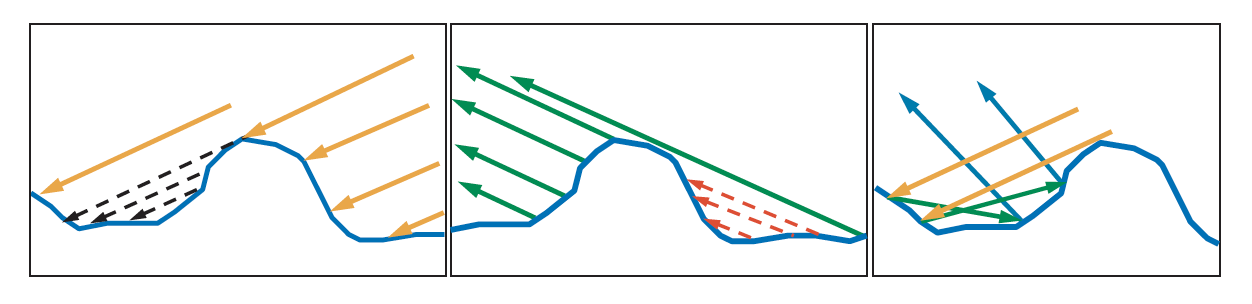
\includegraphics[scale=0.65]{microgeometria}}
                \caption{Representaci\'on gr\'afica de la sombra y el enmascaramiento en la funci\'on de geometr\'ia}
            \end{figure}
    
            % La funci\on de distribuci\'on de las normales, aproxima la cantidad de microfacetas aproxima la alineadas con el
            % vector h, el medio entre el rayo de luz y el punto del vista. El par\'ametro que modela la rugosidad de una superficie
            % afecta en gran medida al resultado. Este es el factor m\'as caracter\'istico del modelo de microfacetas.
            % La funci\'on de geometr\'ia describe la cantidad de rayos ocluidos por las propias microfacetas.\\
    
            % Finalmente, la ecuaci\'on de fresnel describe el ratio de reflexi\'on de una superficie bajo diferentes \'angulos de
            % incidencia.\\
    
    \section{Modelo de Disney 2012}
    Los modelos de BRDF basados en aspectos f\'isicos ofrecen gran versatilidad al conseguir representar gran cantidad de materiales de una
    forma muy realista. Por contra, resultan en una defici\'on del material compleja, con gran cantidad de par\'ametros que resultan poco intuitivos para los artistas.\\
    
    En 2012, Disney presenta su modelo conocido como \textit{Principled} \autocite{disney12}, que, a pesar de ser basado en f\'isica, sigue una serie de directivas
    como tener la menor cantidad de par\'ametros posibles, ofrecer nombres y rangos de par\'ametros amigables para los artistas u ofrecer
    combinaciones robustas y plausibles para todas sus posibles combinaciones. Desde entonces, los materiales basados en f\'isica
    han ganado popularidad y se han introducido progresivamente en la industria de las pel\'iculas y videojuegos, convirtiendo
    al modelo de Disney en el est\'andar de facto en la actualidad.\\

    \begin{figure}[H]
        \vspace{0.5cm}
        \centering
        \frame{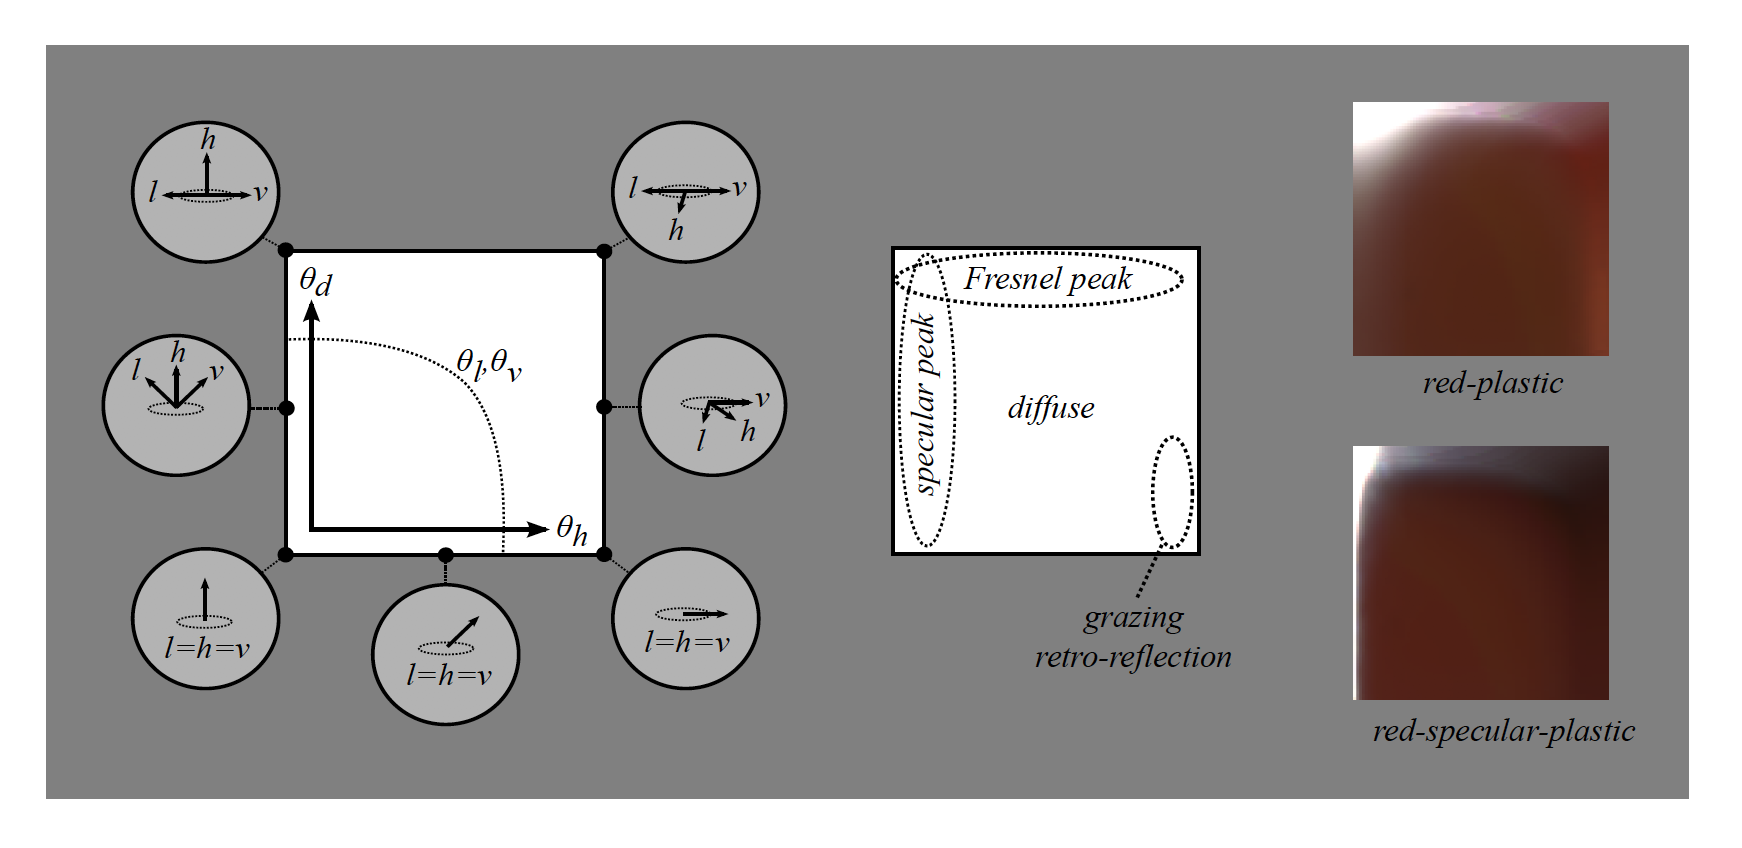
\includegraphics[scale=0.47]{slicespace}}
        \caption{Muestras de materiales MERL, junto a un esquema explicativo de las im\'agenes muestreadas}
        \vspace{0.5cm}
    \end{figure}

    El modelo te\'orico de Disney est\'a basado en las observaciones sobre la tabla MERL \autocite{merl}, que provee una lista
    de 100 materiales muestreados y representados en una gr\'afica cartesiana, cuyo eje $x$ representa pasos discretos de rotaci\'on
    alrededor de la tangente del material y en el $y$, la rotaci\'on alrededor de la normal de la superficie. 

    \begin{figure}[H]
        \vspace{0.5cm}
        \centering
        \frame{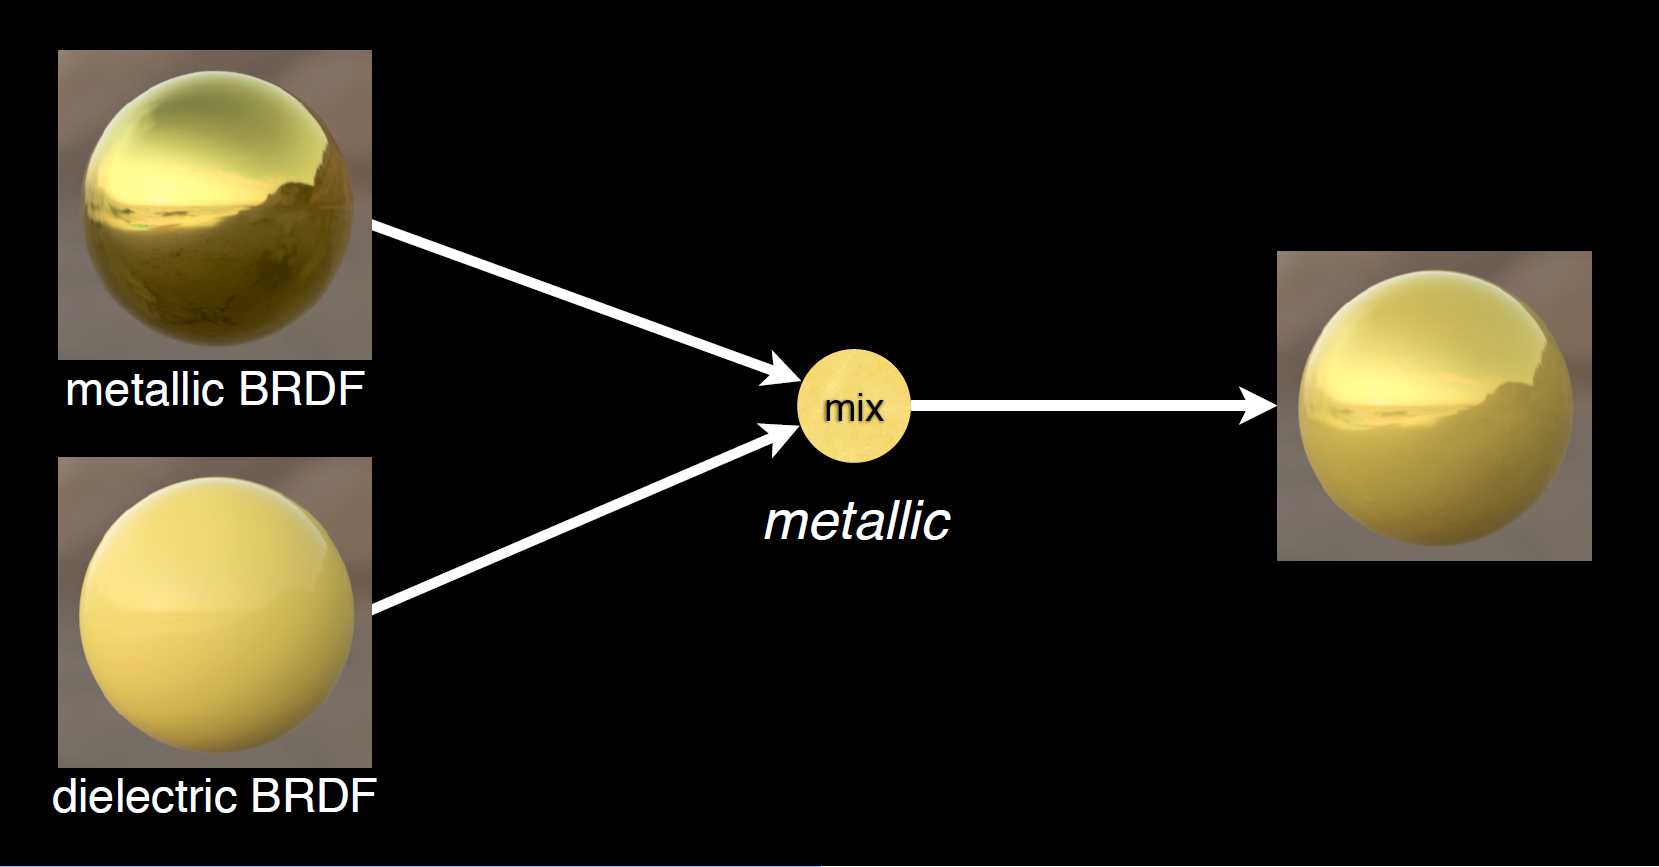
\includegraphics[scale=0.3]{disney12model}}
        \caption{Modelo para met\'alicos y diel\'ectricos de Disney}
        \vspace{0.5cm}
    \end{figure}

    En base a estas observaciones, el modelo \textit{Principled} de Disney, ajusta los t\'erminos del BRDF de Cook-Torrance \autocite{cooktorrance}
    primando la expresividad art\'istica sobre lo f\'isicamente plausible. El modelo aporta dos nuevos l\'obulos que, a diferencia del l\'obulo
    primario pueden variar mucho en forma y tama\~no, adem\'as los tanto los materiales isotro\'opicos como anisotr\'opicos
    se representan con el mismo modelo, que utiliza una interpolaci\'on entre los dos BRDFs, por lo que resulta muy atractivo para los artistas,
    pudiendo representar una enorme variedad de materiales con muy pocos par\'ametros.\\

    La lista de par\'ametros final se compone de: \textit{baseColor}, \textit{subsurface}, \textit{metal}, \textit{specular}, \textit{specularTint},
    \textit{roughness}, \textit{sheen}, \textit{sheenTint}, \textit{clearCoat}, \textit{clearcoatGloss}
    
    % El BRDF de Disney fue presentado por Brent Burley en 2012 y es el utilizado por Disney en sus peliculas de animacion. Es,
    % junto al modelo de Cook-Torrance, el mas utilizado en los motores de tiempo real, sin embargo, el modelo de Burley, es mas
    % amigable para los artistas, a costa de no ser completamente basado en fisica. Los parametros tienen nombres y valores que
    % definen que el aspecto de los materiales son mas intuitivos. Los lobulos adicionales, a diferencia del modelo de Cook-Torrance,
    % pueden variar mucho en forma y tamanho, por lo que es un modelo muy flexible, que permite representar con gran realismo una
    % amplia variedad de materiales.\\
    
    % Es conocido como \textit{principled} por cumplir una serie de m\'aximas, que se respetan en el modelo por encima de las leyes fisicas.
    % El modelo ha de ser intuitivo y no utilizar parametros que se refieran al modelo basado en fisica, debe tener el menor
    % numero de parametros posible, deben de estar normalizados, algunos valores pueden exceder su rango para permitir mayor
    % expresividad y, finalmente, todas las combinaciones de parametros deben de ser robustas y plausibles. Para ello utiliza los
    % par\'ametros: \textit{baseColor}, \textit{subsurface}, \textit{metal}, \textit{specular}, \textit{specularTint}, \textit{roughness},
    % \textit{sheen}, \textit{sheenTint}, \textit{clearCoat}, \textit{clearcoatGloss}
    
    \begin{figure}[H]
        \vspace{0.5cm}
        \centering
          \frame{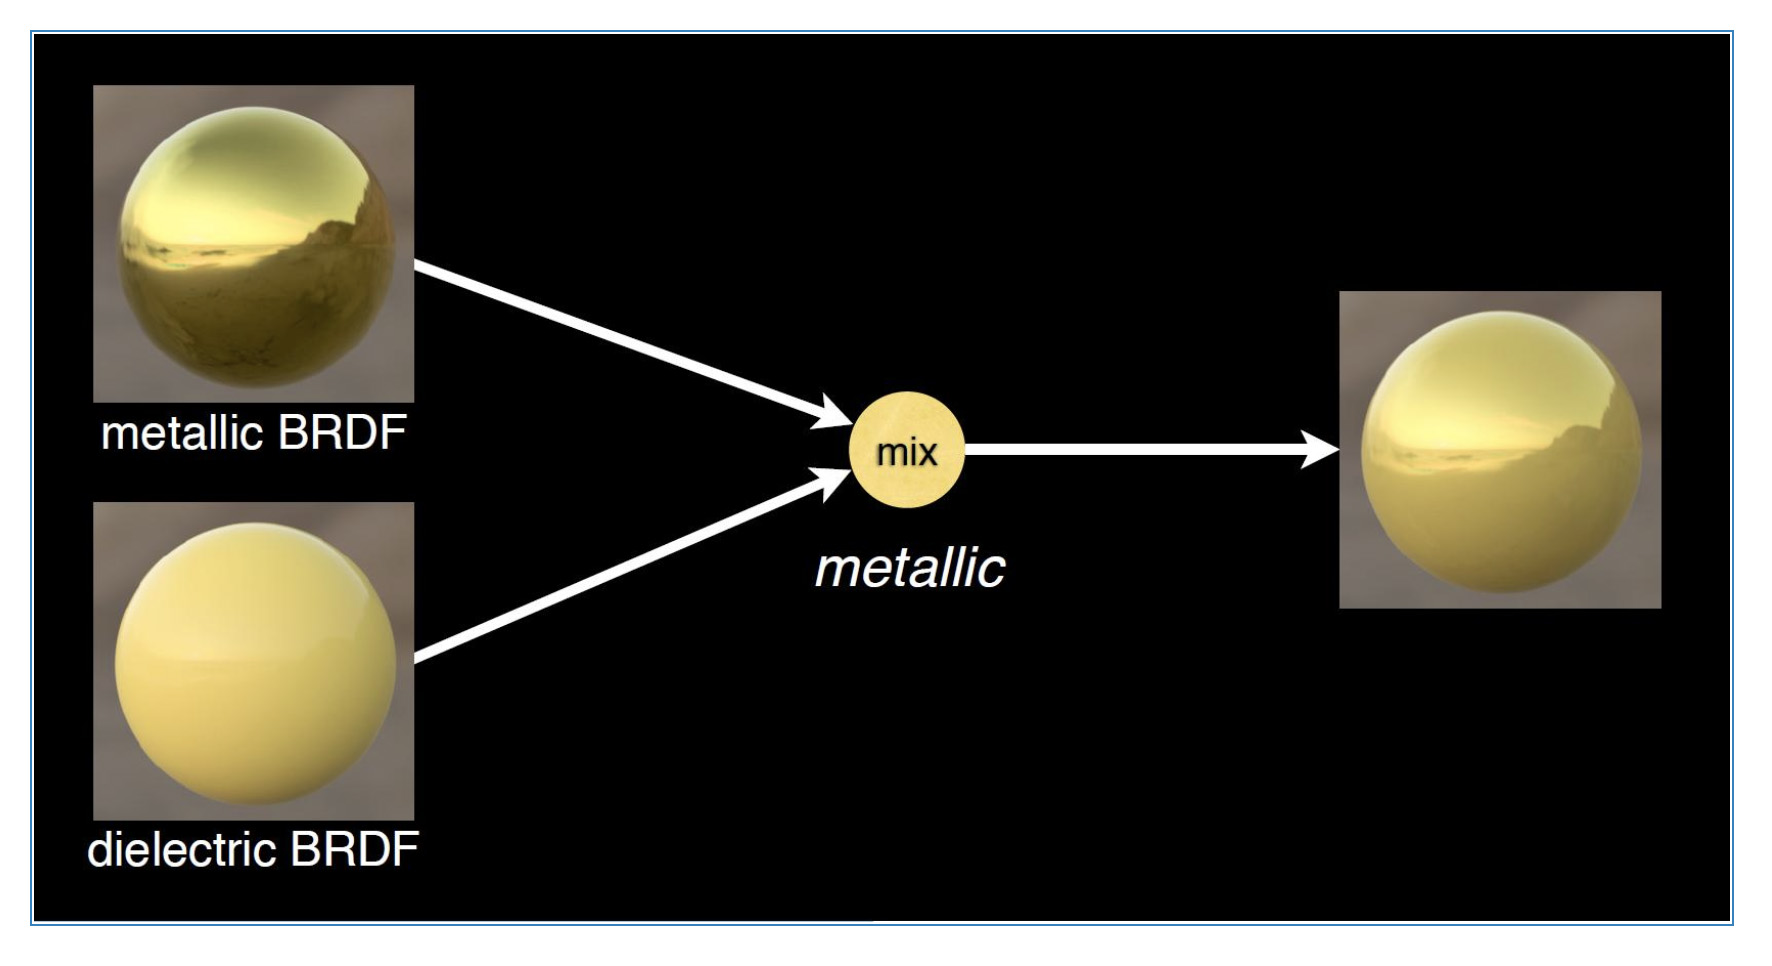
\includegraphics[scale=0.47]{disney}}
        \caption{Modelo de Disney}
        \vspace{0.5cm}
    \end{figure}
    % \begin{itemize}
    % 	\item \textit{baseColor}: el color de la superficie, comunmente utiliza un mapa.
    % 	\item \textit{subsurface}: aproximacion para controlar el color de la reflexion difusa.
    % 	\item \textit{metal}: interpolaci\'on lineal entre los dos modelos. El met\'alico no tiene
    %     componente de reflexi\'on difusa y su componente de reflexi\'on especular es del mismo color que el color base. 
    %     \item \textit{specular}: cantidad de luz incidente reflejada, se utiliza para controlar de forma intuitiva el \'indice de refracci\'on de
    %     una superficie.
    % 	\item \textit{specularTint}: par\'ametro que permite a los artistas controlar el color de la reflexi\'on especular sobre el color
    % 	base.
    % 	\item \textit{roughness}: describe la rugosidad de una superficie, afectando a la reflexi\'on difusa y especular.
    % 	\item \textit{sheen}: permite mayor grado de control sobre la reflexi\'on especular, muy \'util sobre tejidos.
    % 	\item \textit{sheenTint}: color del \textit{sheen}
    % 	\item \textit{clearCoat}: un l\'obulo extra.
    % 	\item \textit{clearcoatGloss}: permite controlar la rugosidad de este l\'obulo.
    % \end{itemize}
        
        \subsection{Componente difusa}
    
        En base a las observaciones sobre los datos de MERL, el modelo difuso parece muy oscuro hacia los bordes, y aplicando
        la funci\'on de Fresnel, para intentar conseguir un modelo f\'isicamente plausible, parece oscurecer m\'as los bordes,
        acentuando el problema.\\
        Disney \autocite{}{disney} utiliza una modificaci\'on del t\'ermino Fresnel-Schlick
        conseguir una dispersi\'on hacia delante y hacia detr\'as que depende del valor de rugosidad del material y se
        adapta mejor a los datos obtenidos de MERL \autocite{merl}.
    
        % \begin{equation}
        %     (1 - F(\theta_l) (1 - F(\theta_d)))
        % \end{equation}
        % \singlespacing
    
        $$
        f_d = \frac{baseColor}{\pi}
        \left(  1 + (F_{D90} - 1)(1 - cos\theta_{wi})^5  \right)
        \left(  1 + (F_{D90} - 1)(1 - cos\theta_{wo})^5  \right)
        $$
    
        \begin{equation}
        \textrm{siendo} \; F_{D90} = 0.5 + 2roughness\cdot{cos^2\theta_d}
        \end{equation}
    
        \singlespacing
        \subsection{Componente especular}
        El modelo de Disney \autocite{disney12} utiliza t\'erminos conocidos del BRDF de Cook-Torrance \autocite{cooktorrance}
        (DFG) e incorpora dos nuevos l\'obulos: el de \textit{sheen} y el de \textit{clearcoat}. El l\'obulo de \textit{sheen}
        permite mayor control sobre la reflexi\'on especular en los \'angulos cr\'iticos, mientras que el l\'obulo de
        \textit{clearcoat} permite simular una capa superficial para imitar efectos el efecto de un barniz o recubrimientos
        transparentes.

            \subsection*{D, t\'ermino de distribuci\'on de las normales}
                La distribuci\'on GGX es equivalente a la de Trowbridge-Reitz, no tiene una cola lo suficientemente larga para la
                mayor\'ia de materiales.

                \begin{equation}
                    D_{TR} = \frac
                    {c}
                    {(\alpha^2 cos^2 \theta_h + sin^2 \theta_h)^2}
                \end{equation}
                \singlespacing

                El modelo de Disney utiliza un exponente en el denominador que permite mayor control sobre el radio de la reflexi\'on
                especular, llamando a \'este t\'ermino Generalized Trowbridge-Reitz, o GTR:

                \begin{equation}
                    D_{GTR} = \frac
                    {c}
                    {(\alpha^2 cos^2 \theta_h + sin^2 \theta_h)^\gamma}
                \end{equation}
                \singlespacing

                Los dos l\'obulos, primario y secundario utilizan la distribuci\'on GTR. El l\'obulo primario,
                que representa la reflexi\'on del material base, utiliza $\gamma = 2$ y puede ser diel\'etrico o met\'alico,
                isotr\'opico o anisotr\'opico. Por otra parte, el l\'obulo secundario representa la capa de \textit{clearcoat}
                sobre el material base, utiliza $\gamma = 1$ y suele ser isotr\'opico y no met\'alico.\\

            \subsection*{F, t\'ermino de Fresnel}
                Para el especular, la aproximaci\'on de Fresnel-Schlick \autocite{schlick} es lo suficientemente precisa y mucho menos costosa que
                que la ecuaci\'on completa de Fresnel.
    
                \begin{equation}
                    F_{Schlick}(w_o, h) = F_0 + (1 - F_0) (1 - (n\cdot{w_o})))^5
                    $$
                    $$
                    \textrm{siendo}\ F_0 = \frac
                    {(n - 1)^2}
                    {(n + 1)^2}
                    \ y \ n = IOR
                \end{equation}
                \singlespacing
                % \todo[inline]{
                %     En la mayor\'ia de los algoritmos de sombreado, el fresnel se utiliza a nivel de la macrosuperficie,
                %     sin embargo, al aplicar el fresnel sobre la normal de la microfacetas, se consigue un mayor grado de realismo para los valores
                %     altos de \textit{roughness}.
                % }
                $F_0$ representa la reflectancia de una incidencia del mismo \'angulo que la normal. $\theta_d$ es el \'angulo
                entre el vector $h$, y el de vista $w_o$. Es acrom\'actico para los diel\'ectricos y crom\'atico para los metales.\\
    
            \subsection*{G, t\'ermino de geometr\'ia}
                % \todo[inline]{Basado en la t\'ecnica de Smith \autocite{smith}}
                % \todo[inline]{
                %     El t\'ermino de geometr\'ia tiene en cuenta las dos cosas, la sombra
                %     y el enmascaramiento. La sombra representa que una microfaceta no es visible desde la direcci\'on de la luz, mientras que el
                %     enmascaramiento significa que una microfaceta no es visible desde la direcci\'on de vista y, por tanto, no contribuyen
                %     a la reflexi\'on.
                % }
                El t\'ermino de geometr\'ia utilizado en el modelo Disney \autocite{disney12} es el Smith-GGX \autocite{ggx}, remapeando el valor de \textit{roughness} para evitar
                ganar demasiada energ\'ia hacia los bordes de materiales brillantes. El l\'obulo primario utiliza un valor $\alpha$
                de rugosidad, mientras que para el l\'obulo de \textit{clearcoat} se utiliza un valor fijo de $\alpha = 0.25$.\\

                Los t\'erminos de geometr\'ia basados en la t\'ecnica de Smith \autocite{smith} separan la funci\'on de geometr\'ia en dos partes.
                La oclusi\'on puede deberse a la sombra, cuando una microfaceta no es visible desde la direcci\'on de la luz o al enmascaramiento,
                cuando no es visible desde la direcci\'on de la vista.
                % utiliza dos modelos diferentes, uno para el l\'obulo primario y otro para el de clearcoat.
                % Para el l\'obulo primario, utiliza e
    
                $$
                G(l, v, h) = G_{GGX}(l)G_{GGX}(v)
                $$
    
                $$
                G_{GGX}(v) = \frac
                {2 (n \cdot{v})}
                {(n \cdot{v}) + \sqrt{ \alpha^2 + (1 - \alpha)^2 (n \cdot{v})^2 }}
                $$
                \singlespacing
                \begin{equation}
                \alpha = (0.5 + roughness / 2)^2
                \end{equation}
                \singlespacing
    
                Para el l\'obulo secundario se utiliza un valor fijo de $\alpha = 0.25$.\\
    
            \subsection*{L\'obulo de \textit{sheen}}
                El l\'obulo de \textit{sheen} utiliza dos par\'ametros para ajustar la intensidad y el color del brillo especular
                en los \'angulos cr\'iticos. Este control es muy \'util para modelar efectos de retroreflexi\'on caracter\'isticos
                de algunos tipos de tejidos.
                % El par\'ametro de \textit{sheen} ofrece un mayor control sobre la reflectancia especular, permitiendo crear materiales con
                % especulares en dos tonos. Mientras que ThreeJs utiliza un BRDF diferente cuando el par\'ametro de \textit{sheen}, en el
                % BRDF de Disney 2012 el \textit{sheen} se modela como otro l\'obulo adicional adem\'as del de \textit{clearcoat}.\\
            
                \begin{eqfloat}[!htb]
                \begin{equation}
                    f(\textit{sheen}, \theta_d) = \textit{sheen} * ((1 - \textit{sheenTint}) + \textit{sheenTint} * \textit{tint}) * (1 - \cos\theta_d)^5
                \end{equation}
                \caption{L\'obulo adicional de \textit{sheen} en Disney 2012}
                \end{eqfloat}
                \singlespacing

            \subsection*{L\'obulo de \textit{clearcoat}}
                El l\'obulo de \textit{clearcoat} es otro l\'obulo adicional que se controla con los par\'ametros \textit{clearcoat}
                y \textit{clearcoatGloss}. Este l\'obulo utiliza el mismo BRDF que el l\'obulo primario pero con modificaciones
                en sus t\'erminos para evitar a\~nadir complejidad a la definici\'on del material.\\

                La funci\'on de distribuci\'on de las normales tambi\'en utiliza $\gamma = 1$ en el modelo GTR.\\

                \begin{eqfloat}[!htb]
                    \begin{equation}
                    D_{GTR} = \frac
                    {c}
                    {(\alpha^2 cos^2 \theta_h + sin^2 \theta_h)}
                    \end{equation}
                    \caption{Funci\'on de distribuci\'on de las normales para el l\'obulo de \textit{clearcoat} en Disney 2012}
                \end{eqfloat}
                \singlespacing

                La funci\'on de Fresnel utiliza el \'indice de refracci\'on fijo de 0.04, o lo que es lo mismo, $F_0 = 0.04$, el valor
                del poliuretano.\\

                $$
                F_{Schlick}(w_o, h) = F_0 + (1 - F_0) (1 - (n\cdot{w_o})))^5
                $$
                \begin{eqfloat}[!htb]
                    \begin{equation}
                        \textrm{siendo}\ F0 = 0.04
                    \end{equation}
                    \caption{Funci\'on de distribuci\'on de las normales para el l\'obulo de \textit{clearcoat} en Disney 2012}
                \end{eqfloat}
                \singlespacing



                % El efecto de \textit{clearcoat}, se utiliza para simular efectos de barniz o recubrimientos, y se aplican tanto en Disney
                % 2012 como un l\'obulo secundario. Mientras que en ThreeJs se utiliza el mismo BRDF con la misma parametrizaci\'on que para
                % el l\'obulo primario, en Disney 2012, var\'ia la parametrizaci\'on de los t\'erminos D y G.\\
    
    \section{Iluminaci\'on indirecta en entornos interactivos}

    % \todo[inline]{
    %     Los motores de renderizado en tiempo real deben utilizar algoritmos lo menos costosos posibles para garantizar un buen
    %     tiempo de respuesta. Es por ello que sus BRDFs, pueden ser m\'as sencillos que los implementados en sistemas de \textit{path-tracing},
    %     ofreciendo una soluci\'on de compromiso entre el rendimiento y los fen\'omenos f\'isicos representados por el modelo.\\
        
    %     Por otra parte, resolver la parte integral de la ecuaci\'on de render:
    
    %     \begin{center}$L_o(p, w_o) = \int_{\Omega} f_r(p, w_i, w_o)L_i(p, w_i)n\cdot{w_i}dw_i$\end{center}
    %     \singlespacing
    %     requiere lanzar rayos no en una direcci\'n si no desde todas las posibles direcciones sobre la semiesferea $\Omega$, por
    %     lo que no es posible en tiempo real, sin embargo, m\'as adelante analizaremos t\'ecnicas que p\'ermiten simular \'este
    %     efecto utilizando c\'alculos precomputados o aproximando la soluci\'on de forma anal\'itica.\\
    % }

    % \todo[inline]{
    %     These effects contribute
    %     greatly to increasing the realism in a rendered image, and provide cues that
    %     help the viewer to understand spatial relationships. At the same time, they are also
    %     complex to simulate and might require precomputations or rendering multiple passes
    %     that compute some intermediate information.
    % }

    La ecuaci\'on de render describe la radiancia de salida sobre un punto.
    \begin{equation}
    L_o(p, w_o) = \int_{\Omega} f_r(p, w_i, w_o)L_i(p, w_i)n\cdot{w_i}dw_i
    \end{equation}
    \singlespacing
    
    Siendo $\Omega$ la semiesfera centrada en el punto sobre el que se calcula la irradiancia, $f_r$ representa el BRDF, $Li$,
    la irradiancia de la escena, y $n\cdot{w_i}$, el coseno entre la normal de la superficie y el de la luz incidente.
    
    \begin{figure}[H]
        \vspace{0.5cm}
        \centering
          \frame{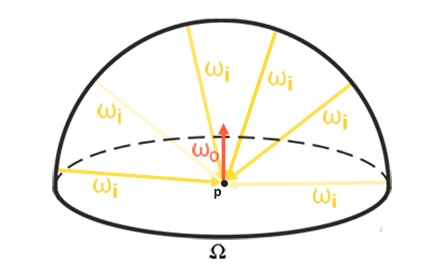
\includegraphics[scale=0.5]{hemisphere}}
        \caption{El c\'aculo de iluminacion indirecta necesita hallar la irradiancia proviniente en todas direcciones $w_i$ sobre la semiesfera $\Omega$.}
      \end{figure}
      \singlespacing

    Calcular la parte integral de la ecuaci\'on requiere lanzar rayos no en una direcci\'on si no desde todas las direcciones posibles
    sobre la semiesfera $\Omega$, por lo que no es posible en tiempo real. En esta secci\'on se repasan t\'ecnicas que precomputan
    los c\'alculos o utilizan funciones anal\'iticas para lograr aproximar este efecto en entornos interactivos.\\

    El primer paso es separar el BRDF en sus componentes especular y difusa, que permitir\'a la combinaci\'on de diferentes
    t\'ecnicas para calcular la soluci\'on de la ecuaci\'on de render.\\

    \begin{equation}
    L_o(p, w_o) = \int_{\Omega} (k_d \frac{c}{\pi} + 
    k_s \frac{DFG}{4(w_o\cdot{n})(w_i\cdot{n})})L_i(p, w_i)n\cdot{w_i}dw_i
    \end{equation}
    \singlespacing
    
    Siendo $k_s$ y $k_d$ t\''erminos independientes, el c\'alculo de la integral se puede separar en partes, la
    integral de la componente difusa m\'as la integral de la componente especular. 
    
    \begin{equation}
    L_o(p, w_o) = \int_{\Omega}
    (k_d \frac{c}{\pi}) L_i(p, w_i)n\cdot{w_i}dw_i +
    \int_{\Omega} 
    k_s \frac{DFG}{4(w_o\cdot{n})(w_i\cdot{n})})L_i(p, w_i)n\cdot{w_i}dw_i
    \end{equation}
    \singlespacing
    
        \subsection{Componente difusa}
        La soluci\'on de la integral de la irradiancia sobre la semiesfera $\Omega$ requiere samplear el entorno
        en todas las direcciones posibles. Es por ello que en tiempo real, la soluci\'on consiste en
        precomputar este c\'alculo.\\
    
        Habiendo separado la ecuaci\'on para la componente difusa y especular, podemos observar que el t\'ermino del difuso
        de Lambert es constante y lo podemos sacar de la integral.
    
        \begin{equation}
        L_o(p, w_o) = \int_{\Omega}
        (k_d \frac{c}{\pi}) L_i(p, w_i)n\cdot{w_i}dw_i=
        k_d \frac{c}{\pi} \int_{\Omega}
        (L_i(p, w_i)n\cdot{w_i}dw_i
        \end{equation}
        \singlespacing
    
        Las t\'enicas IBL (\textit{Image Based Lighting}), permiten precalcular la irradiacia del entorno tratando el entorno
        como un gran emisoror de luz, utilizando una imagenes de referencia para aproximar la luz emitida por el entorno sobre
        el punto que estamos calculando.\\

            \subsection*{Mapas de irradiancia}
            Los mapas de irradiancia utilizan \textit{cubemaps} para muestrear en coordenadas esf\'ericas en pasos discretos la radincia
            procedente del entorno. La irradiancia se estima como la media de la radiancia en todas las direcciones $w_i$ sobre la
            semiesfera $\Omega$ orientada en direcci\'on a la normal de la superficie, $N$. Una vez preconvolucionado el mapa de
            entorno, el resultado, conocido como mapa de irradiancia se almacena en una textura a la que se accede en tiempo
            de ejecuci\'on para consultar los resultados precalculados de irradiancia debida al entorno.

            % % y almacenarla en una nueva textura, el mapa de irradiancia. Para ello se 
            % \todo[inline]{
            %     Convolution is applying some computation to each entry in a data set considering all other entries in the data set;
            %     the data set being the scene's radiance or environment map. Thus for every sample direction in the cubemap, we take
            %     all other sample directions over the hemisphere $\Omega$ into account.
            %     To convolute an environment map we solve the integral for each output wo sample direction by discretely sampling a
            %     large number of directions wi over the hemisphere $\Omega$ and averaging their radiance. The hemisphere we build the sample
            %     directions wi from is oriented towards the output wo sample direction we're convoluting.
            % }
            % \todo[inline]{
            %     computed sum of all indirect diffuse light of the scene hitting some surface aligned along direction wo. Such a
            %     cubemap is known as an irradiance map seeing as the convoluted cubemap effectively allows us to directly sample the
            %     scene's (pre-computed) irradiance from any direction wo.
            % }

            \begin{figure}[H]
                \vspace{0.5cm}
                \centering
                \frame{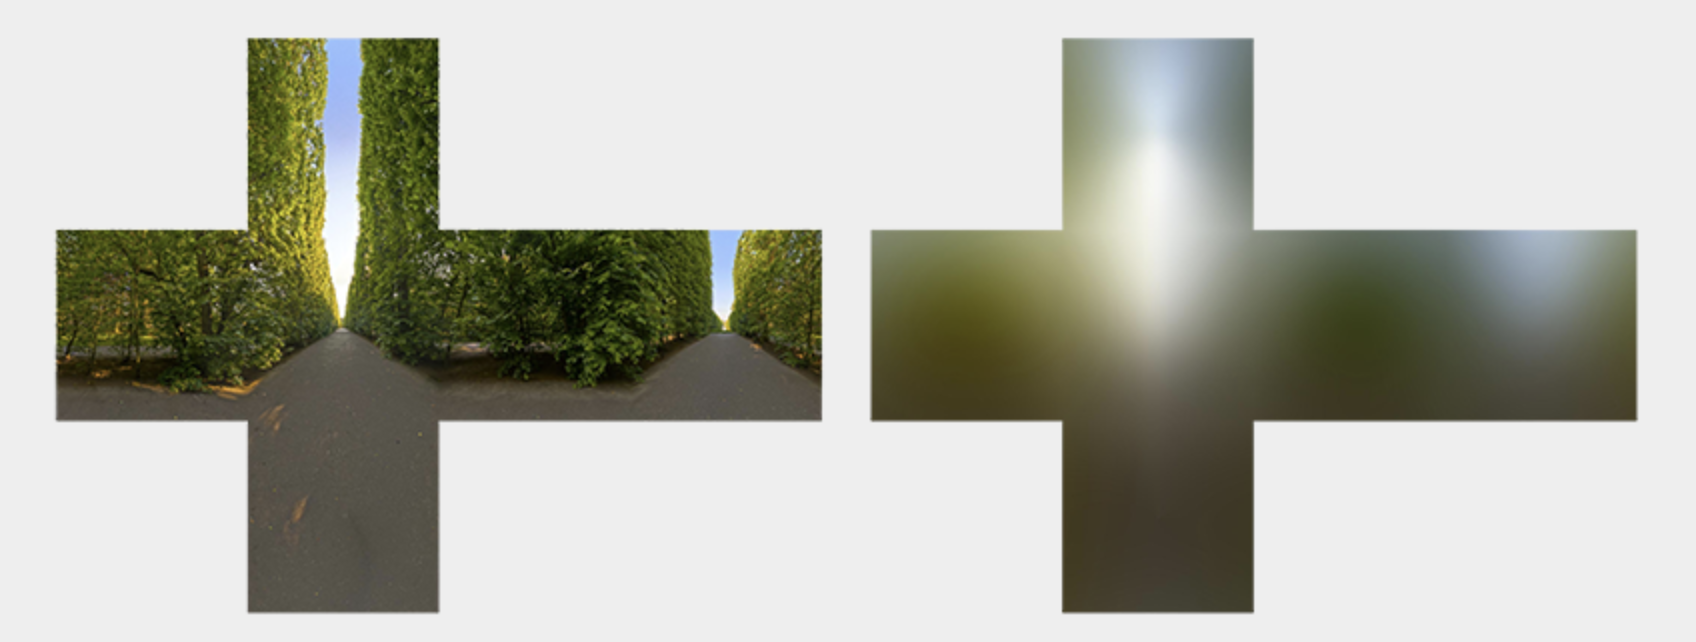
\includegraphics[scale=0.5]{irradiance_map}}
                \caption{Mapa de irradiancia como \textit{cubemap}}
            \end{figure}
            \singlespacing

            \subsection*{Esf\'ericos harm\'onicos}
            La t\'ecnica de esf\'ericos harm\'onicos \autocite{sh} supone una optimizaci\'on sobre la t\'ecnica de mapas de irradiancia,
            que, pese a ser muy eficientes para operaciones de lectura, la convoluci\'on necesaria para generarlos tiene un coste alto.
            Los esf\'ericos harm\'onicos permiten una aproximaci\'on a la irradiancia debida al entorno comprimiendo la informaci\'on
            en una representaci\'on de espacio frente a frecuencias. De esta forma, la informaci\'on se almacena en la funci\'on de
            esf\'ericos harm\'onicos y para consultarla, se utiliza su transformada inversa, que devuelve los datos a su repesentaci\'on espacial.

            % \todo[inline]{
            %     \url{https://developer.nvidia.com/gpugems/gpugems2/part-ii-shading-lighting-and-shadows/chapter-10-real-time-computation-dynamic}
            % }

        \subsection{Componente especular}
        El m\'etodo split-sum approximation presentado por Epic \autocite{unreal}, permite separar la integral en dos partes, la integral de
        la radiancia de la escena y la del BRDF. De forma similar a la componente difusa, precomputar los resultados y consultarlos y para
        calcular el resultado de la integral durante en tiempo real.\\
        
        \singlespacing
        \begin{equation}
            L_o(p, w_o) =
            \int_{\Omega}L_i(p, w_i)dw_i * \int_{\Omega}fr(p, w_i, w_o) n\cdot{w_i}dw_i
        \end{equation}
        \singlespacing

        De forma similar al mapa de irradiancia, el mapa de entorno prefiltrado se precomputa con una convoluci\'on sobre el mapa
        de entorno. La convoluci\'on utiliza la distribuci\'on de normales de Cook-Torrance \autocite{cooktorrance} en funci\'on
        de la direcci\'on de la vista, la normal y la rugosidad del material.\\

        Dado que se desconoce la direcci\'on de la vista al precomputar la radiancia, la aproximaci\'on de asume $w_i = w_o$, lo que implica perder las
        reflexiones especulares en el \'angulo cr\'itico, pero generalmente se considera una aproximaci\'on lo suficientemente buena para entornos
        interactivos. Los resultados para diferentes niveles de rugosidad se almacenan en diferentes \textit{mipmaps} de la textura.\\

        
        \begin{figure}[H]
            \vspace{0.5cm}
            \centering
            \frame{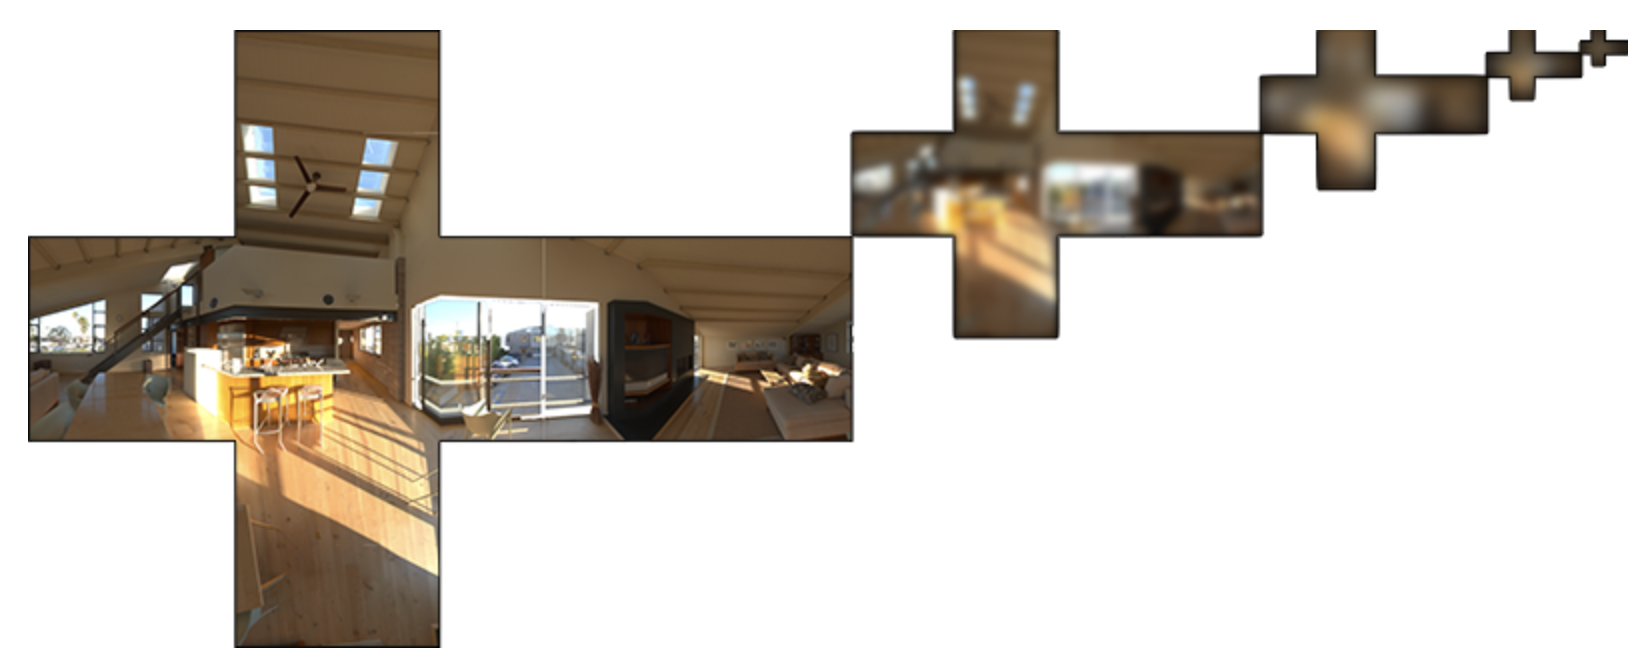
\includegraphics[scale=0.5]{prefilteredenvmap}}
            \caption{Niveles de mipmap del mapa de entorno prefiltrado en funci\'on de la rugosidad del material}
        \end{figure}
        \singlespacing

        % Para computar el mapa prefiltrado de entorno, de forma similar al mapa de irradiancia, se convoluciona el mapa de entorno
        % y se almacenan los resultados en diferentes niveles de mimaps, en funci\'on a la rugosidad de la textura.

        La segunda parte de la integral se precomputa asumiendo una radiancia blanca pura en todas direcciones, que permite calcular
        todos los posibles valores del BRDF en funci\'on de la normal de la superficie, el punto de vista y el valor de rugosidad del material.
        El resultado se almacena en un \textit{look-up texture} (LUT) que se conoce como \textit{BRDF integration map} y contiene
        valores de la escala del Fresnel en el canal rojo de la textura y valores de la desviaci\'on del Fresnel en el canal verde.
        Este LUT se consulta en tiempo de ejecuci\'on se consulta esta tabla, accediendo a sus valores utilizando rangos normalizados entre
        0 y 1 en los dos ejes, utilizando el coseno entre la vista y la normal de la superficie para el eje $x$ y valores de rugosidad
        del material en el eje $y$.

        \begin{figure}[H]
            \vspace{0.5cm}
            \centering
            \frame{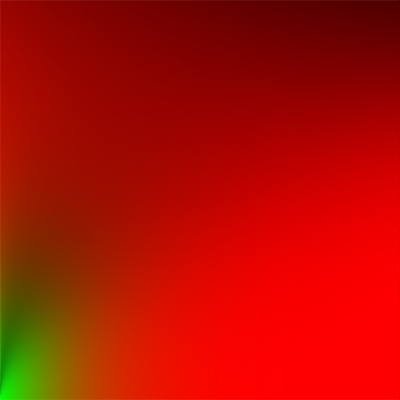
\includegraphics[scale=0.5]{brdf_lut}}
            \caption{\textit{BRDF integration map}}
        \end{figure}
        \singlespacing

        
        En tiempo de ejecuci\'on se accede a esta tabla
        utilizando los valores del coseno entre la direcci\'on de vista y la normal de la superfie en el eje $x$ y utilizando
        el valor de rugosidad del material para el eje $y$ para obtener.\\

        Finalmente el c\'alculo de la integral de la componente especular se ve reducido a una consulta al mapa de entorno prefiltrado,
        otra la \textit{BRDF integration map} y la combinacion de sus resultados:

        \singlespacing
        \begin{lstlisting}[caption=C\'alculo de la componente especular debida al entorno]
float lod = getMipLevelFromRoughness(roughness);
vec3 prefilteredColor = textureCubeLod(PrefilteredEnvMap, refVec, lod);
vec2 envBRDF = texture2D(BRDFIntegrationMap, vec2(NdotV, roughness)).xy;
vec3 indirectSpecular = prefilteredColor * (F * envBRDF.x + envBRDF.y) 
        \end{lstlisting}
        \singlespacing
        
        % un \textit{look-up texture} (LUT), que almacena
        % los c\'alculos precomputados del BRDF para los diferentes valores de \textit{rougness} y del producto escalar $w_i\cdot{n}$.
        % El \textit{BRDF integration map} asume 




        % De la misma forma que para el c\'alculo de la componente difusa, el c\'alculo de la componente especular
    



      \chapter{Desarrollo de infraestructura y servicios web}
Author es la plataforma de Seddi que permite a dise\~nadores, patronistas y dem\'as agentes involucrados en el proceso
de dise\~no y prototipado de una prenda trabajar con r\'eplicas digitales de tejidos sobre un entorno colaborativo web.\\

Un API REST proveee la informaci\'on de los tejidos capturados por Seddi para su representaci\'on en el contexto de Author,
que permite al usuario crear y editar patrones, detalles constructivos u ornamentos de una prenda. Este flujo permite
el dise\~no de una prenda completamente sobre el cliente web, mientras que para las acciones m\'as costosas, como la simulaci\'on
o renderizado basado en trazado de rayos se utilizan los servicios en la nube de Seddi.\\


\begin{figure}[H]
  \vspace{0.5cm}
  \centering
    \frame{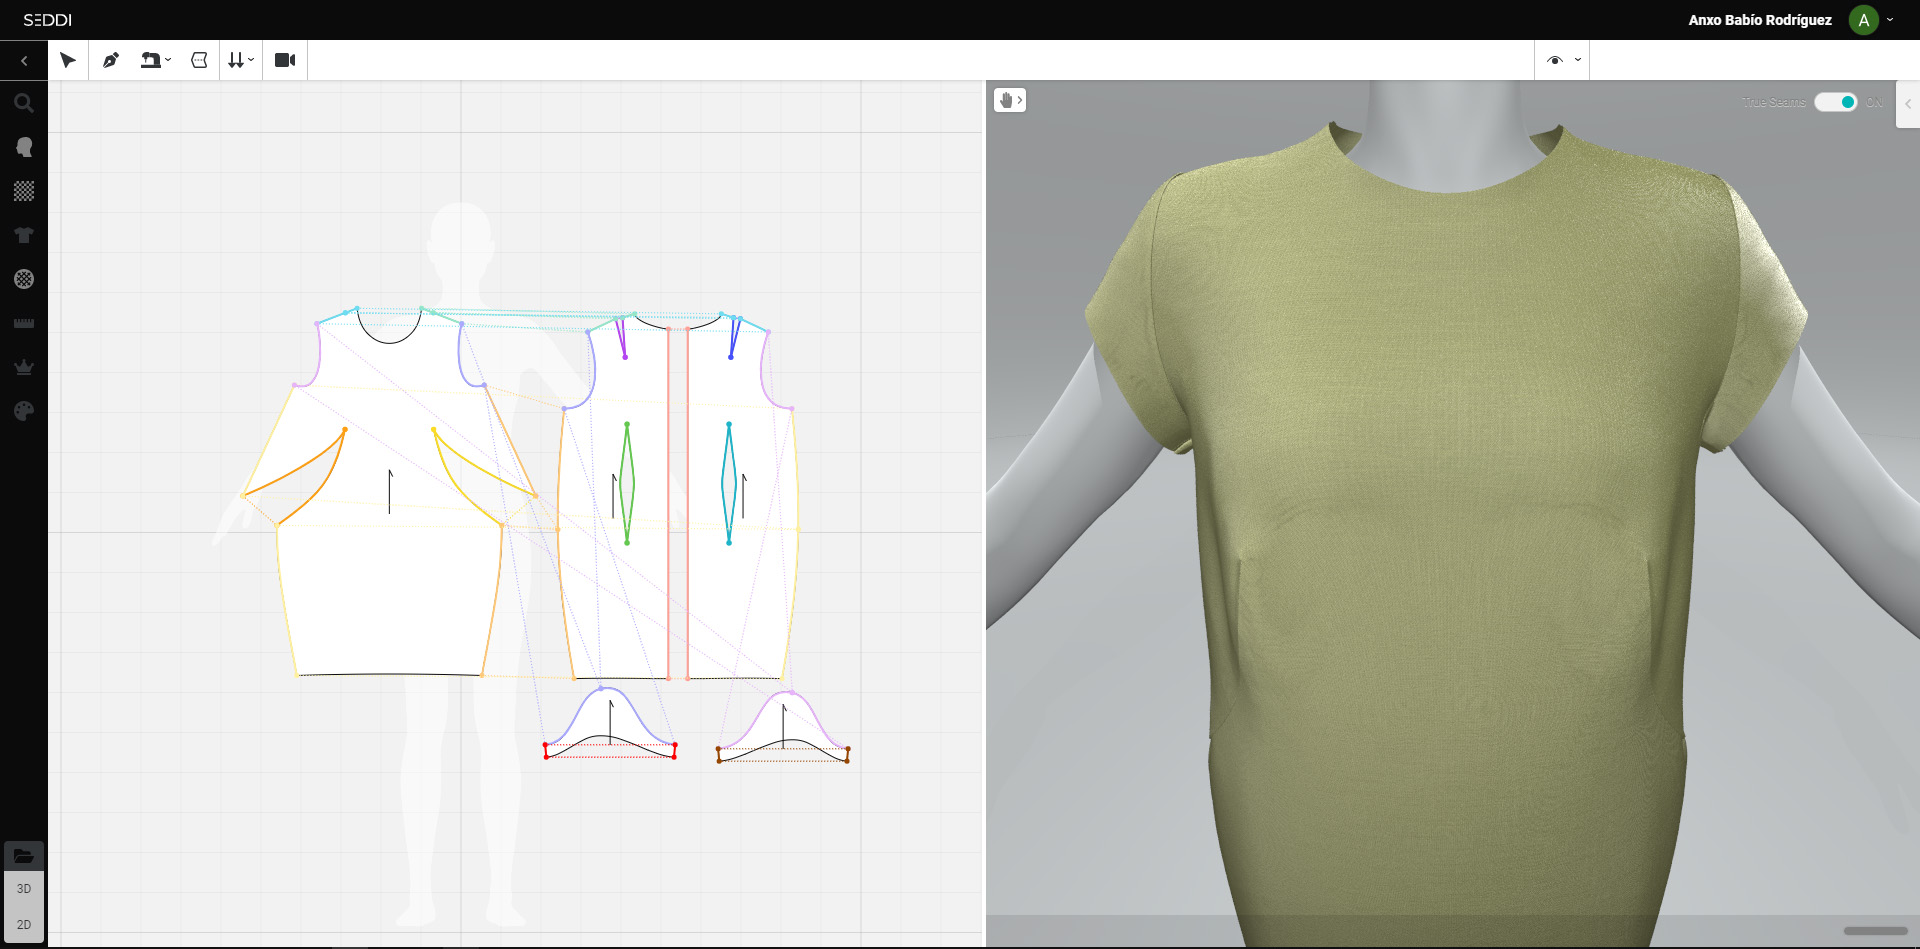
\includegraphics[scale=0.36]{viewports}}
  \caption{Editor de patrones 2D y editor 3D de Author}
\end{figure}

En la primera secci\'on de este cap\'itulo se detallan los cambios requeridos para dar soporte al nuevo modelo en la infraestructura
de Seddi. Por otra parte, la segunda secci\'on ofrece una visi\'on general del sistema de renderizado de ThreeJs, el motor de
renderizado que se utiliza en Author y sobre el que se integrar\'a el nuevo material.
% ofrece una visi\'on general sobre la arquitectura del sistema de renderizado de ThreeJs

% Para trabajar sobre estas r\'eplicas se proporcionan al usuario contextos 2D y 3D, as\'i como paneles de propiedades que
% permiten al usuario editar el patr\'on, detalles constructivos u ornamentos de una prenda. Este flujo permite el dise\~no
% y prototipado de la prenda completamente en el cliente web, mientras que para las acciones m\'as costosas, como la simulaci\'on
% o renderizado basado en trazado de rayos se utilizan los servicios en la nube de Seddi.\\

% Los servicios en la nube utilizan una arquitectura distribuida, diferentes servicios que se comunican entre s\'i para realizar
% una tarea en conjunto. Esta arquitectura implica una mayor complejidad, teniendo que comunicar los diferentes servicios,
% pero ofrece una mayor escalabilidad, tolerancia a fallos y la posibilidad de compartir recursos entre las partes del sistema.\\

% se computan en un servidor \textit{Hight Performance Computing} (HPC) que se reserva bajo demanda.\\

% y utiliza un sistema de cola
% de mensajes para recibir peticiones y enviar los resultados al cliente web

% El cliente web utiliza React para el desarrollo de UI, y ThreeJs y la API nativa de canvas para ofrecer un entorno interactivo.
% Author ofrece principalemente dos dos contextos, un entorno 2D que utiliza el API de canvas y en el que se pueden importar o
% editar patrones y un entorno 3D para previsualizar y editar detalles de disen\~no y constructivos de la prenda.

% Las interacciones de usuario actualizan el estado local del cliente que se comunica con el API REST para persistir los cambios
% sobre los recursos en base de datos. Este flujo permite el dise\~no y prototipado de la prenda completamente en el
% cliente web, mientras que para las acciones m\'as costosas, como la simulaci\'on o renderizado basado en trazado de rayos, se
% computan en un servidor \textit{Hight Performance Computing} (HPC) reservado bajo demanda.\\
% y utiliza un sistema de cola
% de mensajes para recibir peticiones y enviar los resultados al cliente web.

% Author es la plataforma web de Seddi que ofrece a los usuarios la posibilidad de trabajar con r\'eplicas digitales de los tejidos
% para dise\~nar prendas. Para ello se sirve de una infraestructura en la nube que proporciona acceso a los datos de tejidos
% capturados as\' y expone funcionalidades de las tecnolog\'ias de captura y simulaci\'on de Seddi.

% Al contrario que en una arquitectura centralizada, en la que la l\'ogica de negocio se controla en un sistema
% principal, los servicios en la nube utilizan una arquitectura distribuida, diferentes servicios que se comunican
% entre s\'i para realizar una tarea en conjunto. Esta arquitectura implica una mayor complejidad, teniendo que comunicar
% los diferentes servicios, pero ofrece una mayor escalabilidad, tolerancia a fallos y la posibilidad de compartir recursos
% entre las partes del sistema.\\

% Para trabajar con las r\'eplicas digitales de tejidos y tecnolog\'ias de simulaci\'on y renderizado desarrolladas por los
% departamentos de investigaci\'on de Seddi, la plataforma de Author se apoya en una infraestructura de servicios en la nube
% de Seddi.\\

% Los servicios gestionan una colecci\'on de recursos relacionados y exponen su funcionalidad a trav\'es de contratos a
% otros usuarios y servicios parte del sistema




% Las interacciones de usuario actualizan el estado local del cliente que se comunica con el API REST para persistir los cambios
% sobre los recursos en base de datos. Este flujo permite el dise\~no y prototipado de la prenda completamente en el
% cliente web, mientras que para las acciones m\'as costosas, como la simulaci\'on o renderizado basado en trazado de rayos, se
% computan en un servidor \textit{Hight Performance Computing} (HPC) que se reserva bajo demanda y utiliza un sistema de cola
% de mensajes para recibir peticiones y enviar los resultados al cliente web.




% Author es la plataforma web de Seddi que ofrece a los usuarios la posibilidad de trabajar con r\'eplicas digitales de los tejidos
% para dise\~nar prendas. Para ello se sirve de una infraestructura en la nube que proporciona acceso a los datos de tejidos
% capturados as\' y expone funcionalidades de las tecnolog\'ias de captura y simulaci\'on de Seddi.

% El cliente web utiliza React para el desarrollo de UI, y ThreeJs y la API nativa de canvas para ofrecer un entorno interactivo.
% Author ofrece principalemente dos dos contextos, un entorno 2D que utiliza el API de canvas y en el que se pueden importar o
% editar patrones y un entorno 3D para previsualizar y editar detalles de disen\~no y constructivos de la prenda.

% para
% permitir al usuario editar y consultar propiedades del tejido, detalles constructivos, ornamentos, etc. 


% Canvas de HTML para el editor 2D y Three.js como motor de renderizado para el editor de 3D. Las interacciones de
% usuario actualizan el estado local del cliente y se comunica con el API REST para persistir los cambios sobre
% los recursos en base de datos. Este flujo permite el dise\~no y prototipado de la prenda completamente en el
% cliente web, mientras que para las acciones m\'as costosas, como la simulaci\'on o renderizado offline de tejidos,
% se reserva al usuario un servidor que utiliza un servicio HPC de Seddi encarga de recibir, procesar y enviar la
% petici\'on a traves del sistema de cola de mensajes.

% \begin{figure}[H]
%   \vspace{1cm}
%   \centering
%     \frame{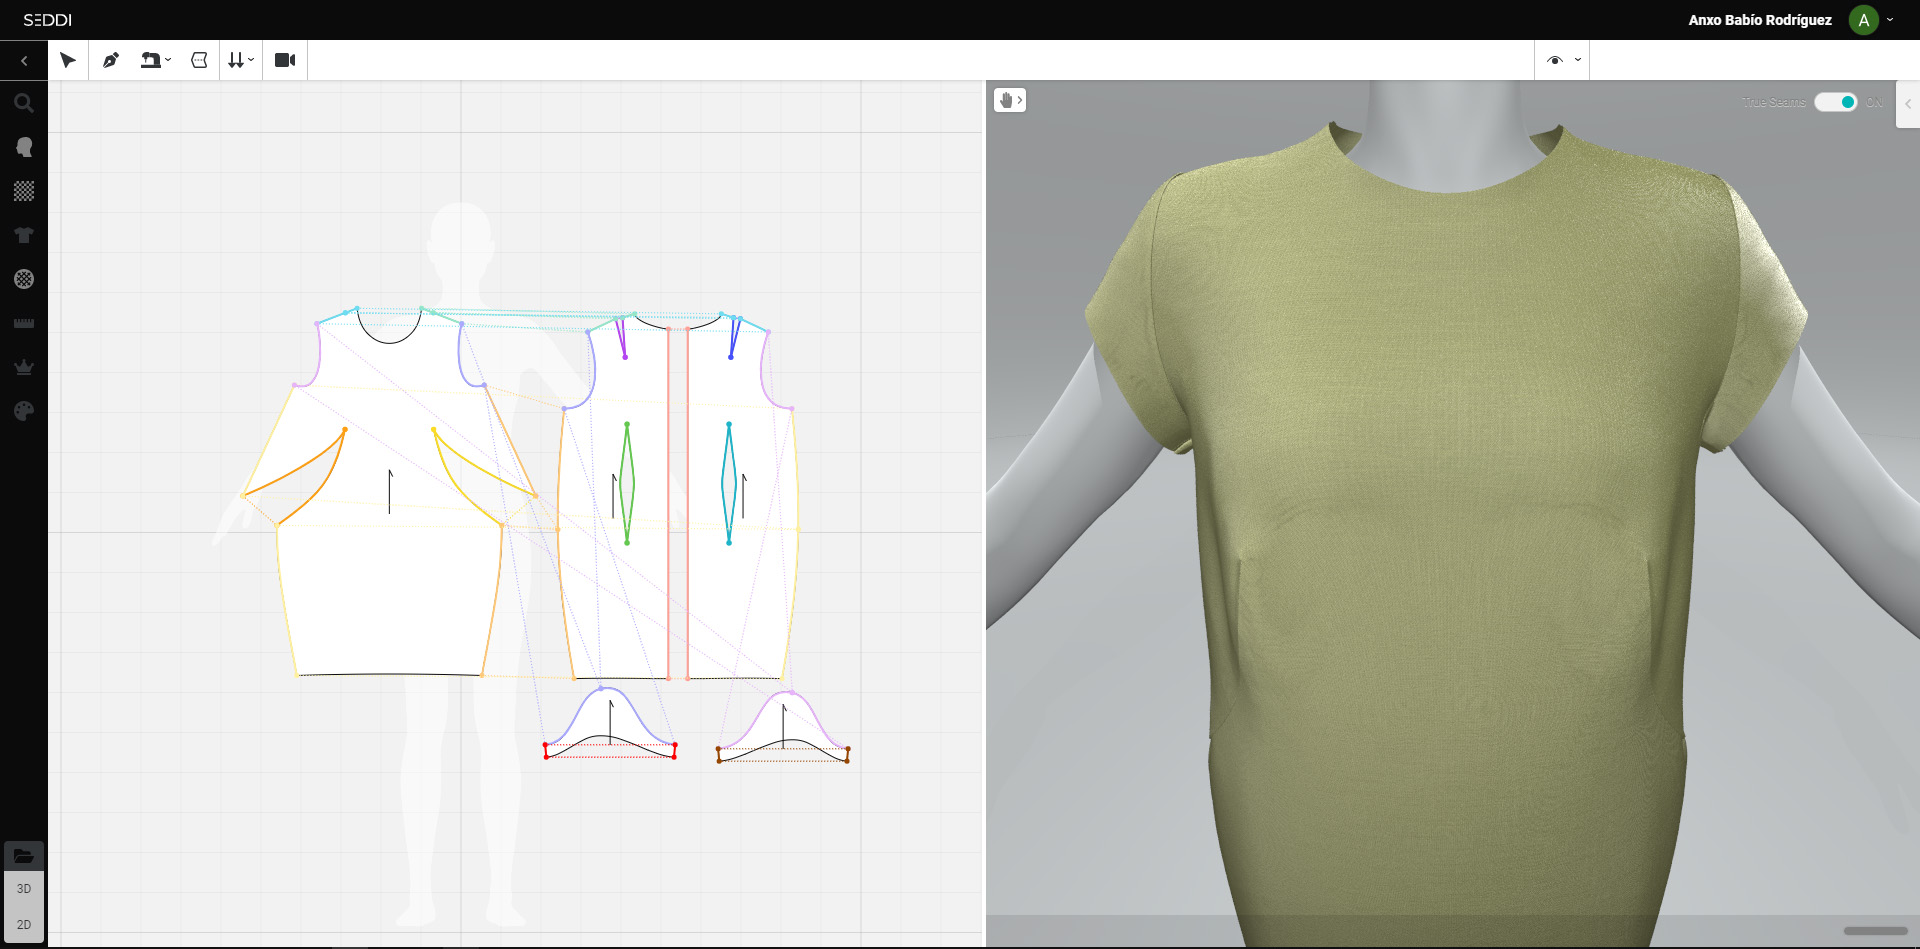
\includegraphics[scale=0.28]{viewports}}
%   \caption{Editor de patrones 2D y editor 3D de Author}
%   \vspace{0.5cm}
% \end{figure}

\section{Servicios en la nube de Seddi}

\bgroup

  Los servicios en la nube utilizan una arquitectura distribu\'ida, diferentes servicios que se comunican entre s\'i para realizar
  una tarea en conjunto. Esta arquitectura implica una mayor complejidad, teniendo que comunicar los diferentes servicios,
  pero ofrece una mayor escalabilidad, tolerancia a fallos y la posibilidad de compartir recursos entre las partes del sistema.

  \begin{figure}[H]
    \vspace{0.5cm}
    \centering
      \frame{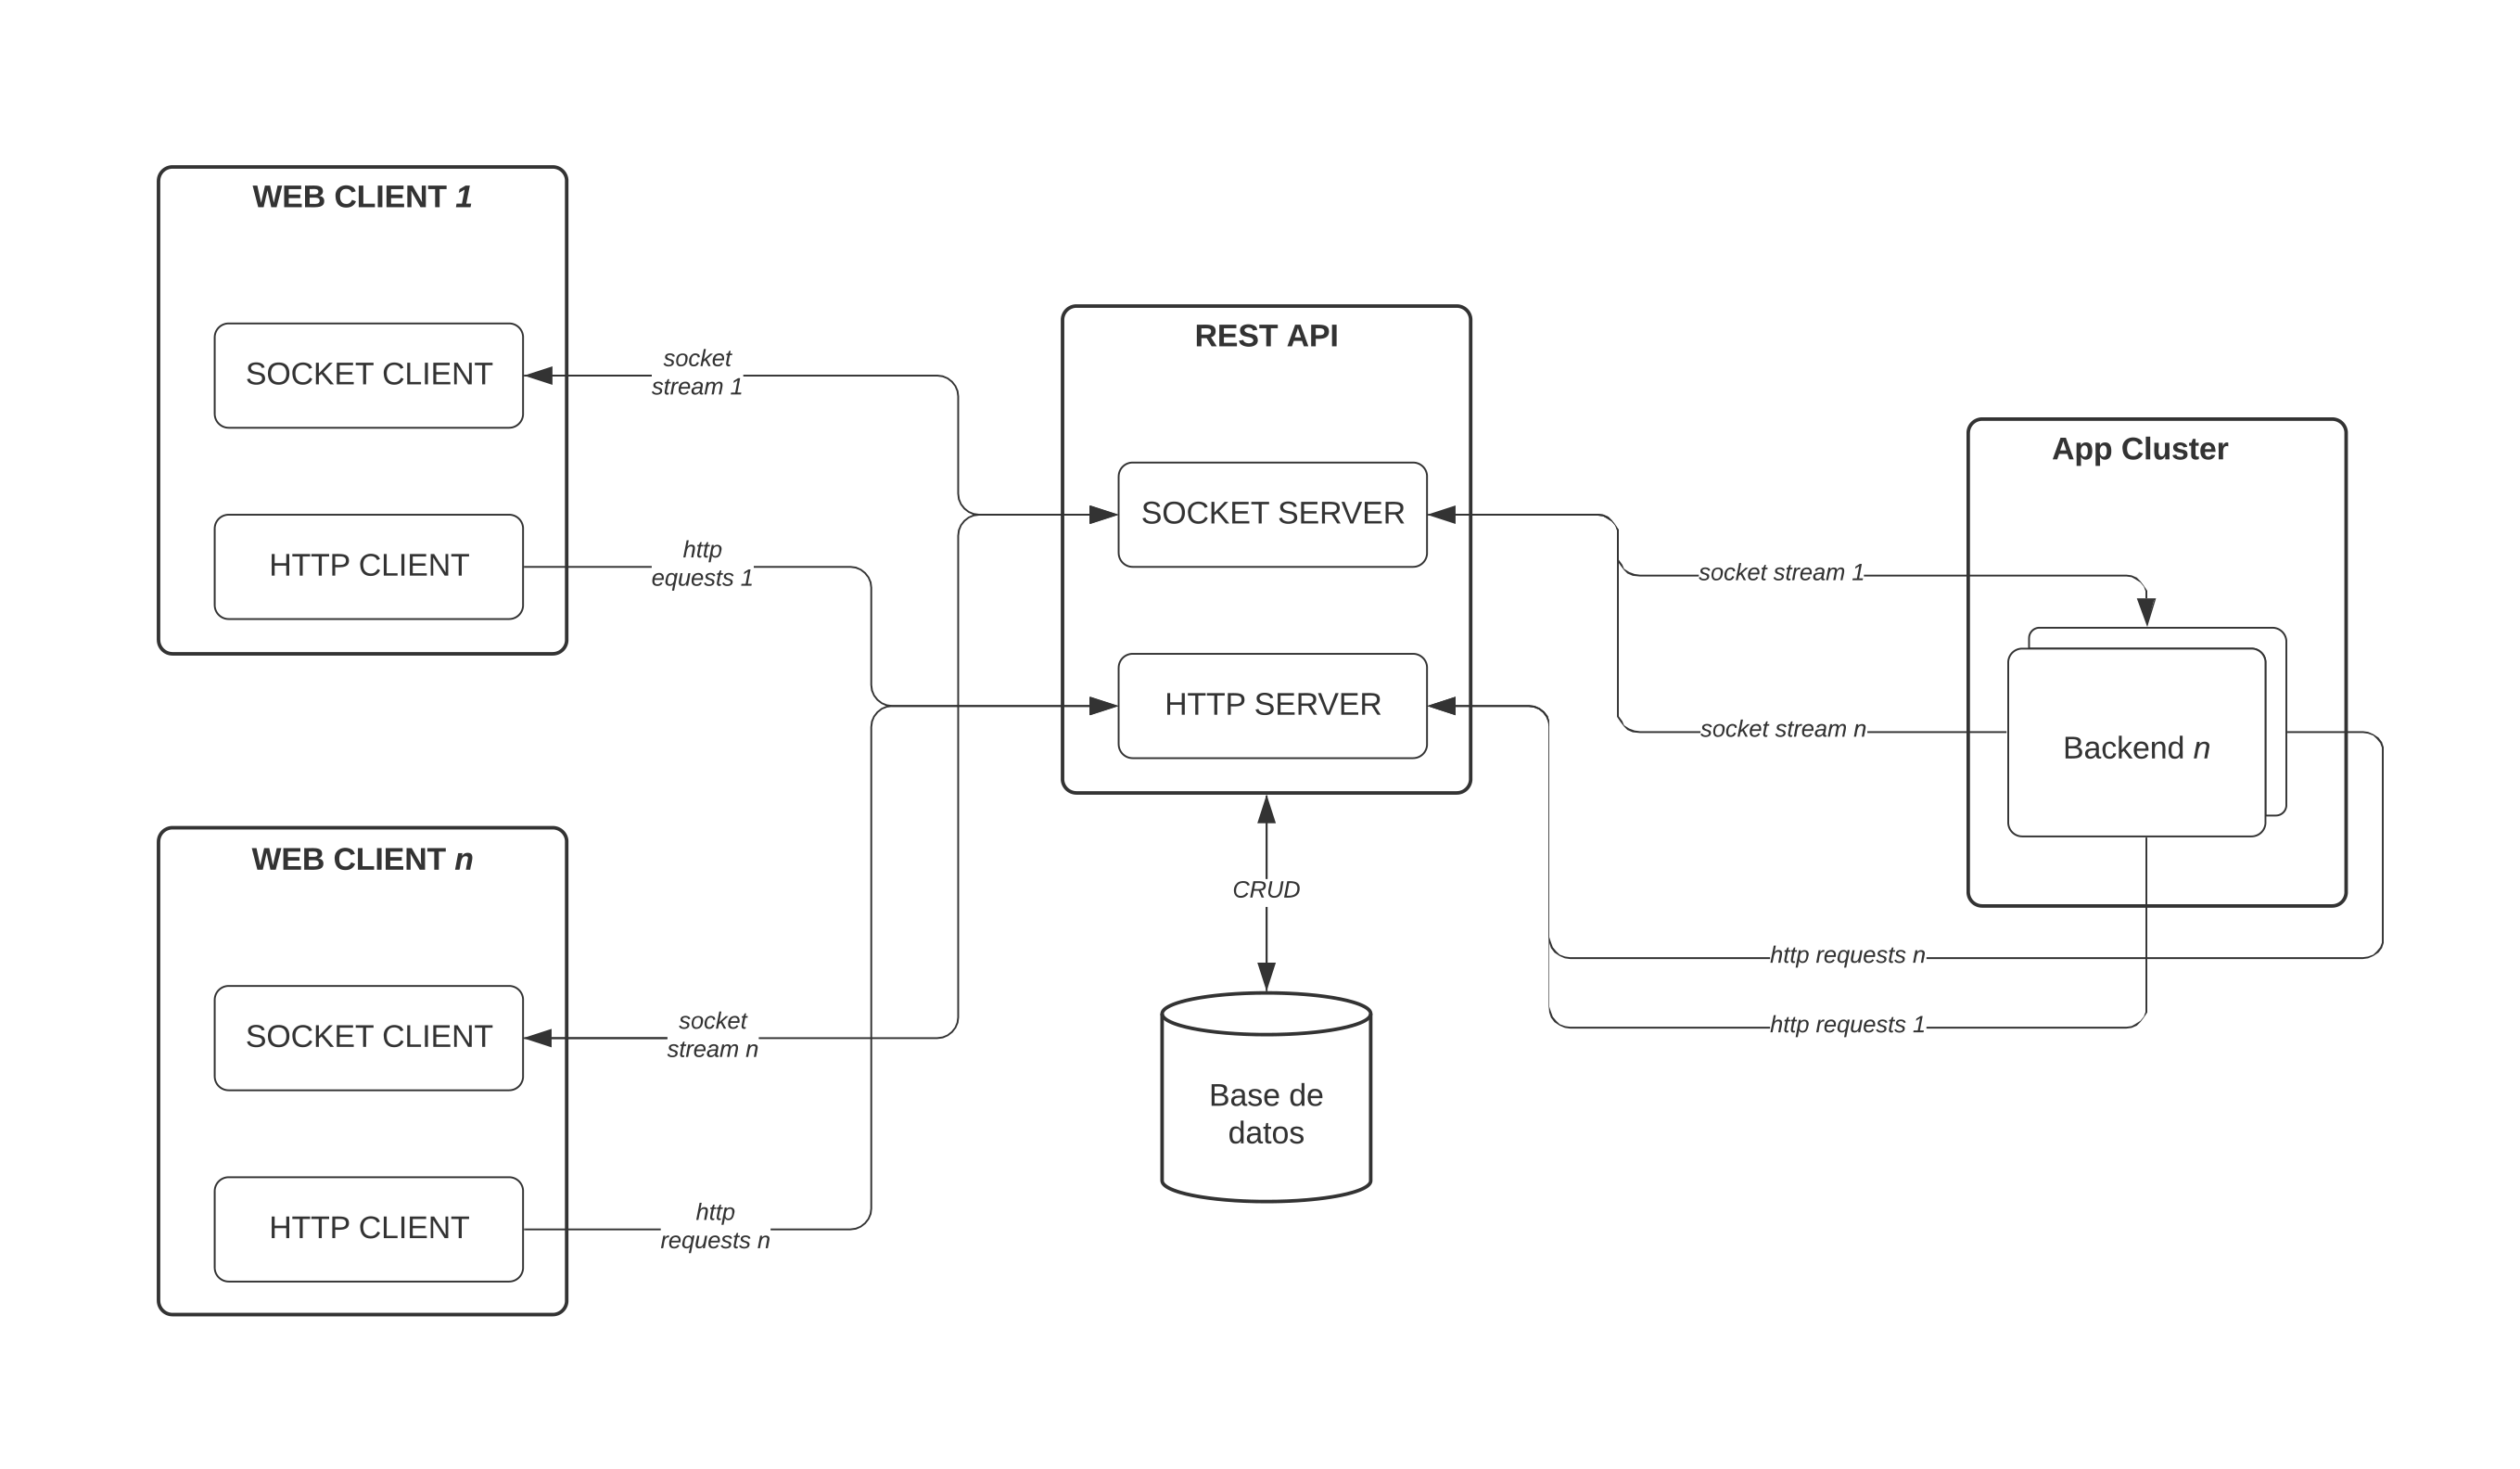
\includegraphics[scale=0.55]{seddi_diagram}}
    \caption{Esquema simplificado de comunicaciones y servicios en Seddi.}
    \vspace{0.5cm}
  \end{figure}

  Seddi ofrece sus servicios a trav\'es de clientes web que exponen la funcionalidad al usuario y se comunican con un API
  REST para gestionar el acceso a recursos compartidos en la plataforma. Para utilizar un nuevo material especializado en tejidos,
  adem\'as de actualizar el motor de renderizado, ha de actualizarse la infraestructura de servicios de Seddi para crear un modelo
  de datos que lo represente en el sistema de almacenamiento de Seddi, as\'i como proveer acceso a \'el a trav\'es del API
  REST. Por otra parte, las acciones m\'as costosas, como la simulaci\'on o el renderizado basado en trazado de rayos, se
  computan en servicios de \textit{Hight Performance Computing} (HPC) que se reservan bajo demanda.


  % la infraestructura ha de soportar su modelo de datos a dem\'as de proveer acceso a \'el a trav\'es del API REST.
  
  % Las operaciones m\'as costasas se ejecutan, bajo demandad,
  % en servicios de \textit{High Performance Computing} (HPC) utilizando un sistema de cola de mensajes.

  % y una conexion de sockets con un sistema de cola de
  % mensajes para pedir y recibir en tiempo real las operaciones graficas mas costosas que se realizan en los servidores en la nube.

\egroup

\subsection{Implementaci\'on del modelo de datos}
Como sistema de almacenamiento de datos Seddi utiliza MongoDB \autocite{mongodb}, un sistema NoSQL basado en documentos. Los sistemas no relacionales
nacieron a mediados de los 90 frente a los sistemas SQL y sus principales ventajas son sus bajos tiempos de respuesta, flexibilidad
en el modelo de datos y escalabilidad horizontal.\\

Para asegurar la consistencia entre los diferentes motores de la compa\~n\'ia, la representaci\'on de los materiales en base de
datos y las interfaces que proporcionan acceso a ellos son comunes. Adem\'as, los motores de renderizado utilizan un \textit{Entity Component System}
(ECS) \autocite{ecs}, las referencias a materiales se serializan como parte de un componente.\\

Los componentes que permiten renderizar elementos con materiales en la escena son \textit{GarmentPieceComponent} y \textit{MeshRenderableComponent}.
\textit{GarmentPieceComponent} se especializa en representar tejidos en la escena y \textit{MeshRenderableComponent}
se utiliza para definir el resto de elementos con materiales como escenarios, avatares, fornituras, etc.

\begin{figure}[H]
  \vspace{0.5cm}
  \centering
    \frame{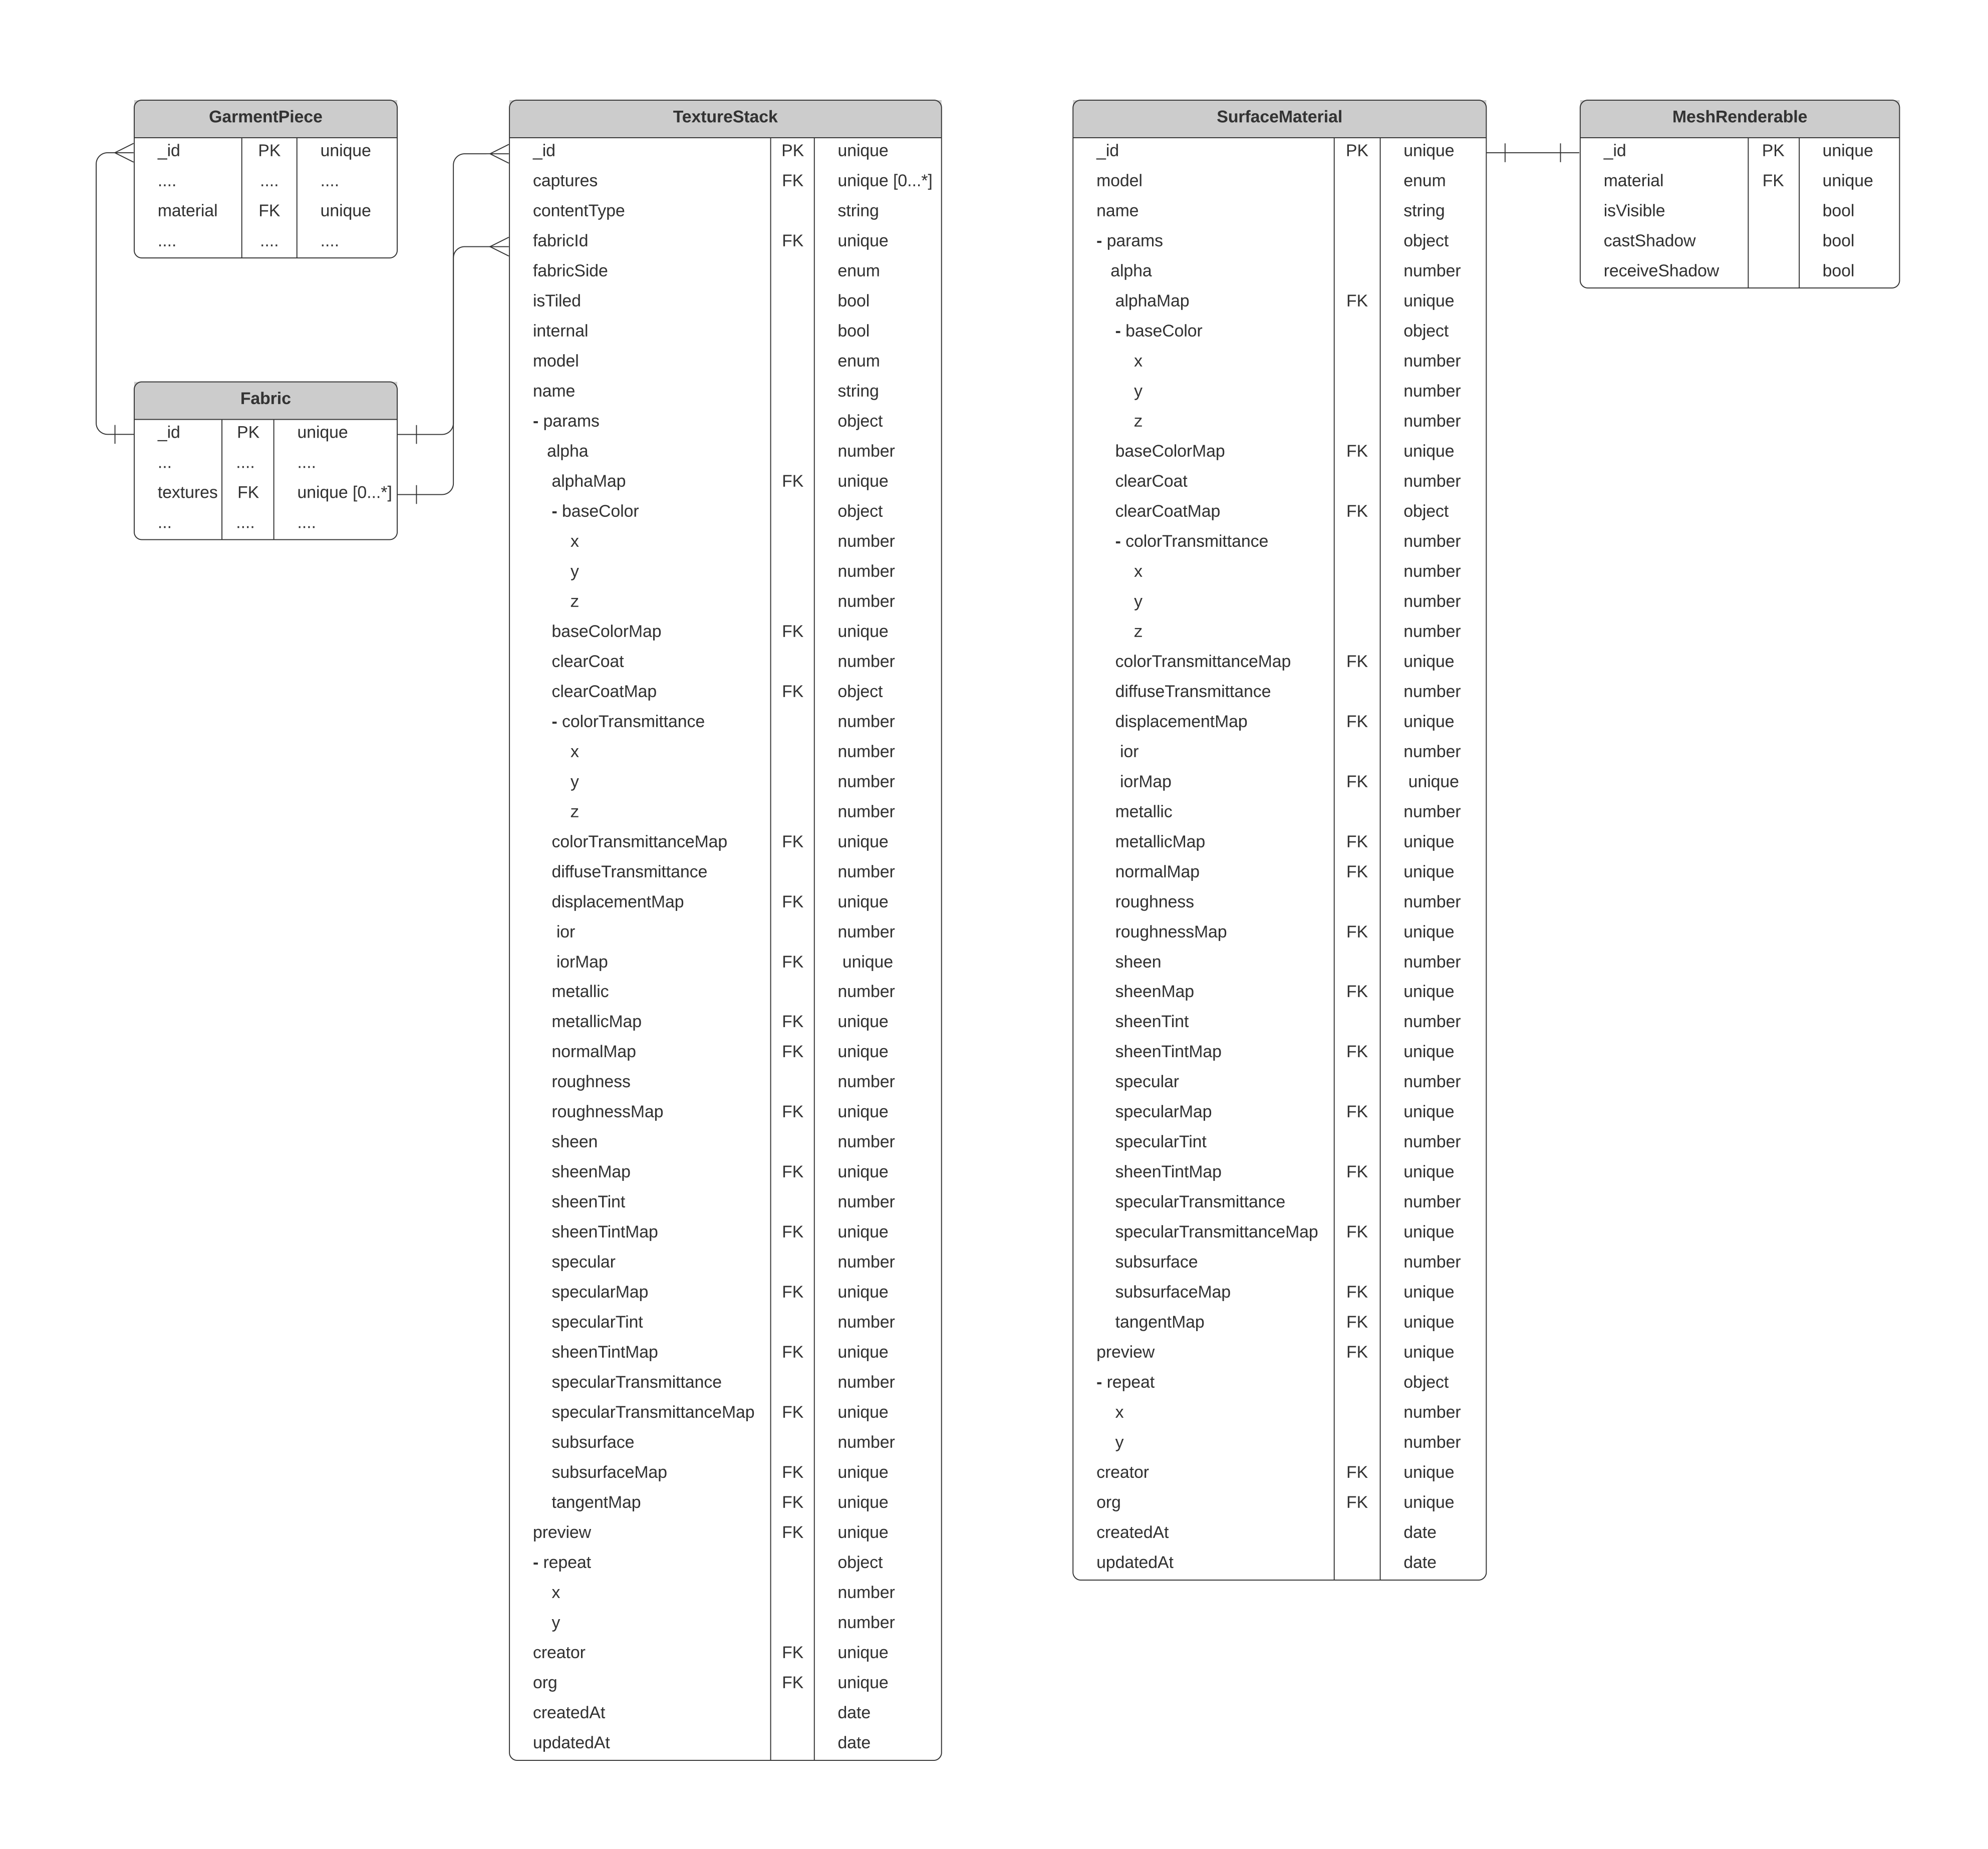
\includegraphics[scale=0.37]{materials_schema}}
  \caption{Modelo de datos de los recursos que soportan materiales.}
  \vspace{0.5cm}
\end{figure}

Los materiales de un \textit{GarmentPieceComponent} se almacenan en el campo \textit{textures} de un recurso \textit{Fabric}. El campo
\textit{textures} es un array que referencia recursos \textit{TextureStack} que contienen las definiciones de los materiales para
la parte frontal y trasera obtenidas durante el proceso de captura \'optica. Por otra parte, los materiales de un \textit{GarmentPieceComponent}
se almacenan en recursos \textit{SurfaceMaterial}. Estos recursos almacenan diferentes tipos de metadatos y pueden utilizar
diferentes modelos de BRDFs pero comparten la parametrizaci\'on de los materiales.

% Mientras que la
% representaci\'on de un material de \textit{GarmentPieceComponent} se almacena bajo el nombre de \textit{TextureStack} y es el
% resultada



% El modelo de datos que representa un material en la infraestructura de Seddi es com\'un a los diferentes motores de renderizado
% de la compa\~n\'ia, de esta forma los motores comparten parametrizaci\'on.

% La informaci\'on de un material para que los motores gr\'aficos del cliente web y los servicios de HPC
% se almacena en un \textit{TextureStack}, que son resultado de la captura \'optica de un tejido, o un \textit{SurfaceMaterial}, la definici\'on para
% cualquier otro elemento de la escena 3D. Ambos motores gr\'aficos utilizan un Entity Component System (ECS), por lo que
% la informacion sobre los materiales son una referencia un \textit{GarmentPieceComponent}, en el caso de un \textit{TextureStack},
% o un \textit{MeshRenderableComponent}, en el caso de un \textit{SurfaceMaterial}.\\



\subsection{Actualizaci\'on de las interfaces de servicios REST}
El API REST que proporciona acceso a los recursos est\'a montada sobre Node \autocite{node}, un entorno de ejecuci\'on de Javascript montado
sobre el motor V8 de Google que proporciona operaciones no bloqueantes de lectura y escritura (I/O) a disco o red.
De entre la variedad de \textit{frameworks} disponibles en el ecosistema de Node, el API REST de Seddi utiliza Express debido
a su amplia comunidad, rendimiento, facilidad y velocidad de desarrollo.\\

\begin{figure}[H]
  \vspace{0.5cm}
  \centering
    \frame{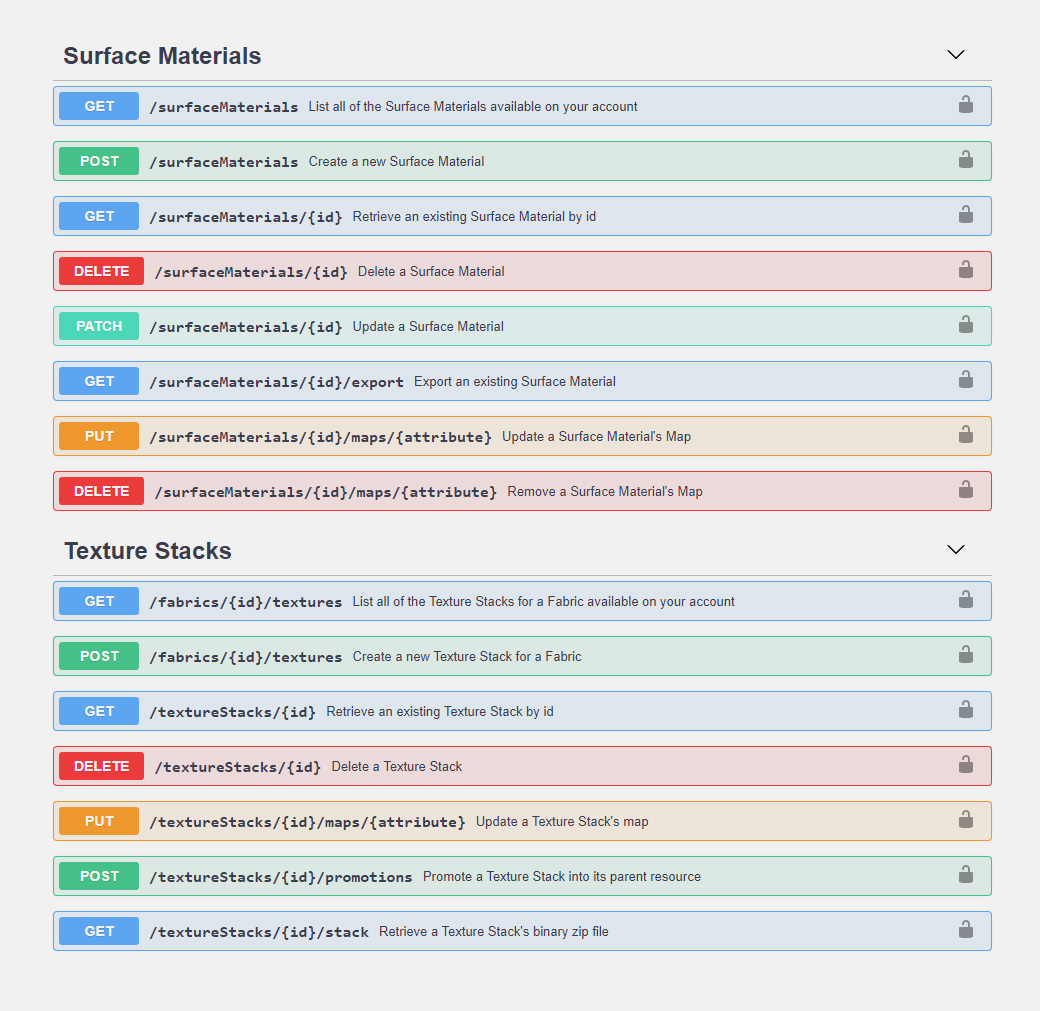
\includegraphics[scale=0.37]{swagger}}
  \caption{Documentaci\'on de los recursos SurafaceMaterial y TextureStack en Swagger.}
  \vspace{0.5cm}
\end{figure}

Las operaciones permitidas sobre los recursos \textit{SurfaceMaterial} y \textit{TextureStack} son: crear, obtener, actualizar y borrar
un recurso por \textit{id}, adem\'as de permitir actualizar la textura de un mapa y descargar la definici\'on del material
y sus texturas. Adicionalmente, un \textit{TextureStack} puede ser promocionado, lo que indica que el recurso indicado
es el que se utiliza dentro del campo \textit{textures} del \textit{Fabric} asociado, que se indica en el campo \textit{fabricId} del
\textit{TextureStack}.\\
\newpage
Las citadas funcionalidades se documentan en Swagger \autocite{swagger}, una herramienta de documentaci\'on automatizada que proporciona una gu\'ia a
a los consumidores del API.

% es la definici\'on
% de material que se utilizar\'a






\section{Motor de renderizado de Author}
% \todo[inline]{
%   % Para trabajar sobre estas r\'eplicas se proporcionan al usuario contextos 2D y 3D, as\'i como paneles de propiedades que
%   % permiten al usuario editar el patr\'on, detalles constructivos u ornamentos de una prenda.
%   Author ofrece un contexto interactivo de edici\'on que permite al usuario la edici\'on de y creaci\'on de patrones, detalles
%   constructivos u ornamentos de una prenda. La edici\'on se realiza a trav\'es de paneles de propiedades, y contextos de 2D
%   y 3D. Este trabajo se centra en el editor 3D para incrementar el realismo de los tejidos y su coherencia con las im\'agenes
%   generadas por el servicio de renderizado basado en trazado de rayos.\\

%   En esta secci\'on se ofrece una visi\'on general sobre la arquitectura de su sistema de renderizado,
%   su librer\'ia de materiales y los matem\'aticos e implementaciones utilizadas por sus materiales PBR.\\
% }
Adem\'as de actualizar el modelo de datos y las interfaces que ofrecen acceso a ellos, el nuevo material ha de ser integrado
dentro del contexto 3D basado en ThreeJs de Author. A continuaci\'on se analiza la arquitectura de su sistema de renderizado,
su librer\'ia de materiales y los modelos matem\'aticos e implementaciones utilizadas por sus materiales PBR.\\

% a\~nadiendo un nuevo material a su librer\'ia
% de materiales est\'andar. 
% Author ofrece dos entornos de edici\'on, un contexto 2D que utiliza el API de canvas y en el que se pueden importar o
% editar patrones y un contexto 3D para previsualizar y editar detalles
% de dise\~no y constructivos de la prenda.\\

% Este trabajo trata de incrementar el realismo del contexto 3D interactivo y mejorar la coherencia
% con el motor de renderizado bajo demanda basado en el trazado de rayos. Con intenci\'on de ofrecer una visi\'on amplia
% sobre ThreeJs, motor en el que se implementar\'a el nuevo modelo de material, 

% A continuaci\'on se explica la arquitectura y el sistema de materiales materiales de ThreeJs.


\subsection{Arquitectura del sistema de renderizado de ThreeJs}
El nuevo material extiende la librer\'ia de materiales para ofrecer una interfaz igual al resto de materiales nativos
de ThreeJs. Para ello, estudiaremos la arquitectura del motor de renderizado de ThreeJs tomando como referencia los dos
materiales disponibles en la librer\'ia, \textit{MeshStandardMaterial} y \textit{MeshPhysicalMaterial}.

\begin{figure}[H]
  \vspace{0.5cm}
  \centering
    \frame{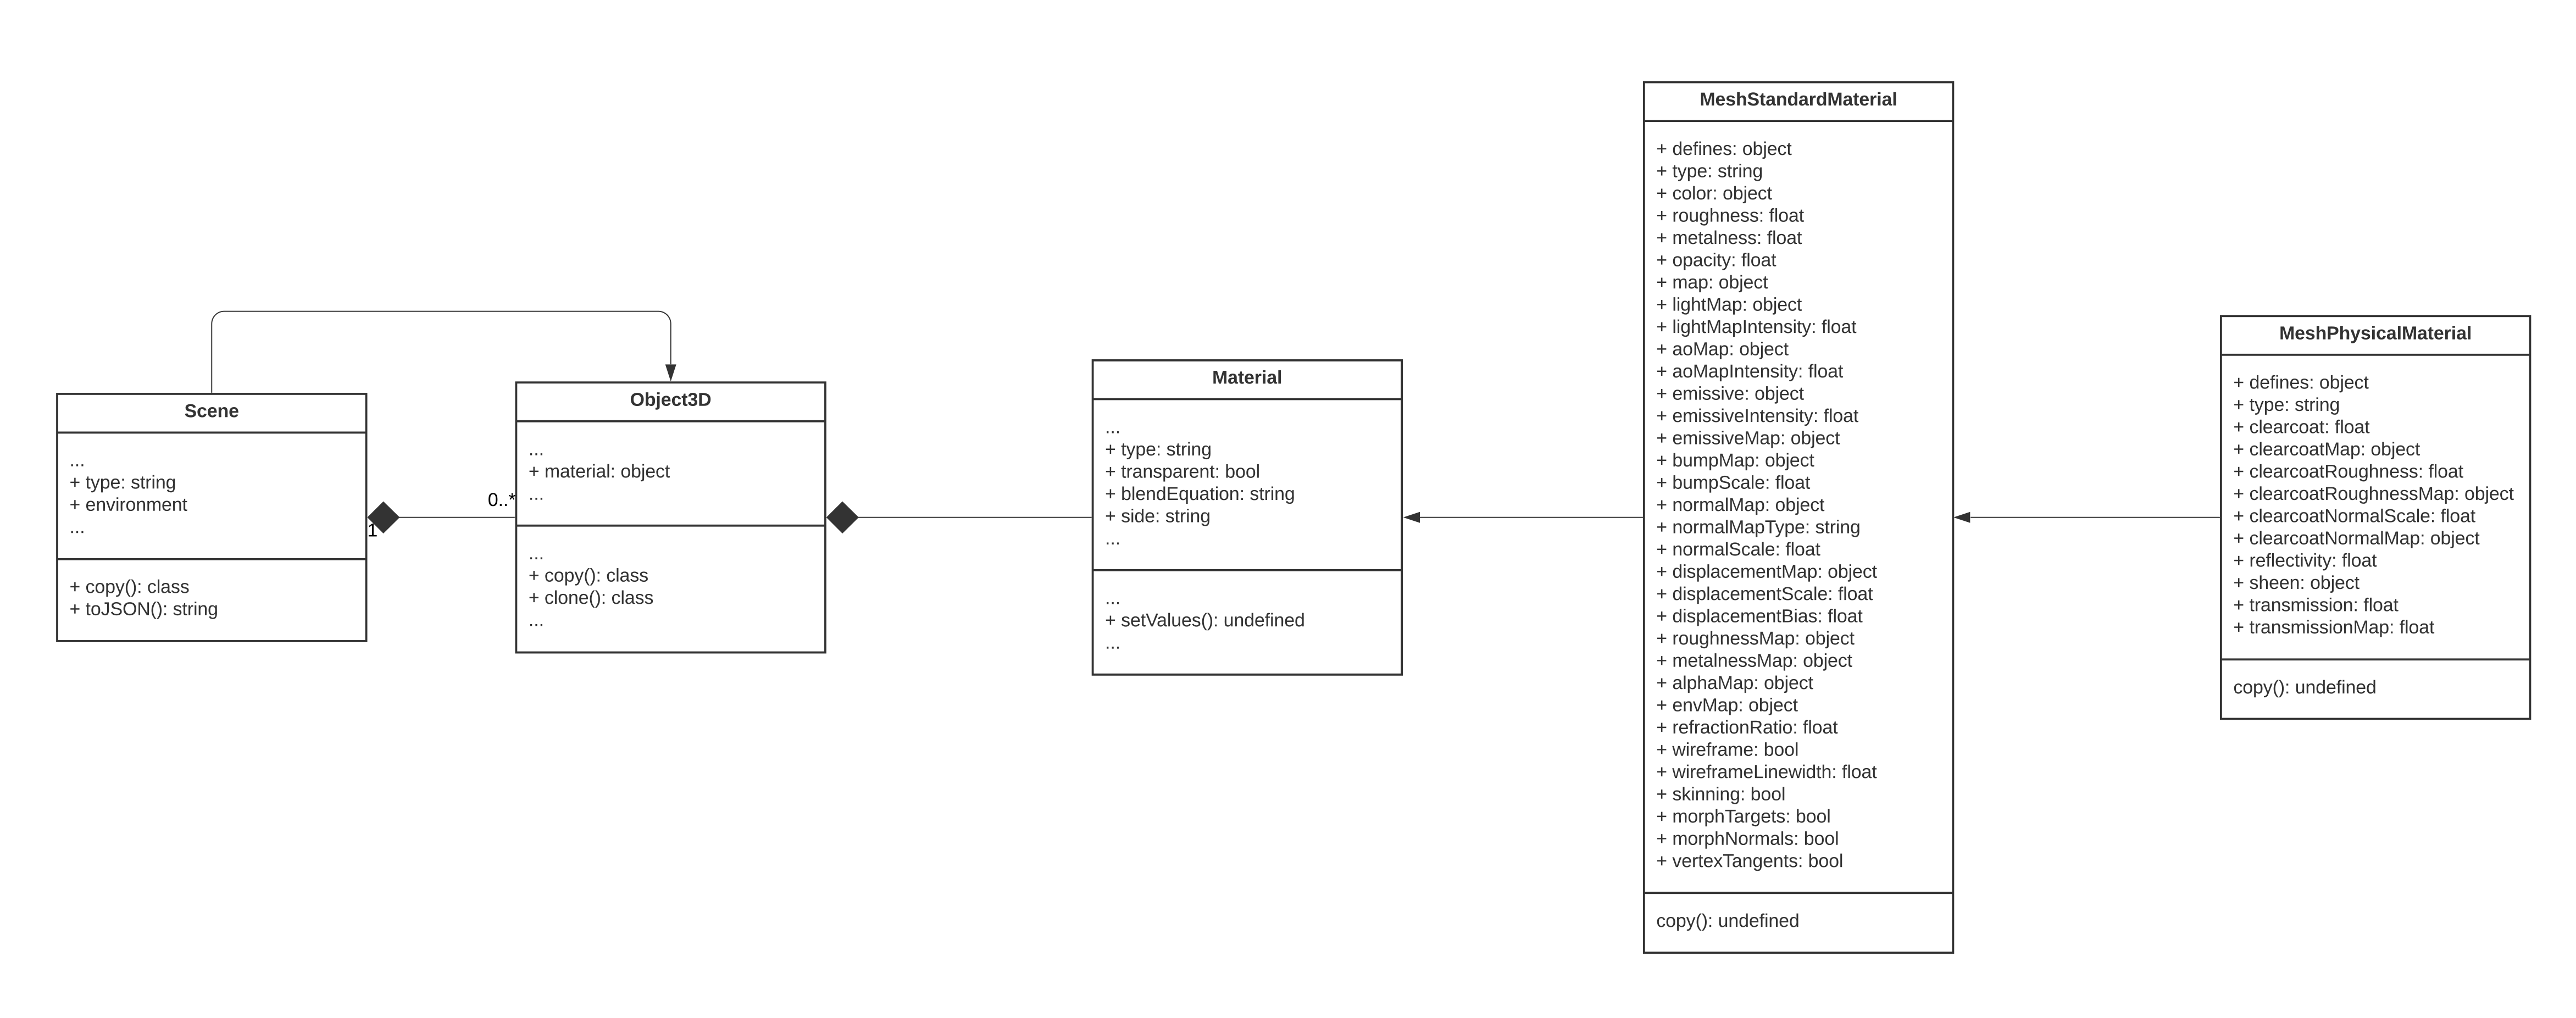
\includegraphics[scale=0.35]{threejs_scenegraph}}
  \caption{Documentaci\'on de los recursos SurfaceMaterial y TextureStack en Swagger.}
  \vspace{0.5cm}
\end{figure}

La clase base de la que heredan es \textit{Material} y almacena informaci\'on com\'un
cualquier tipo de material: opacidad, ecuaci\'on de blending, la cara visible, etc. Adem\'as proporciona un m\'etodo
para configurar los valores de las propiedades del material, as\'i como m\'etodos para la copia, clonado o serializaci\'on
del material.\\

\textit{MeshStandarMaterial} hereda de \textit{Material} y es la implementaci\'on base de un material PBR. Almacena propiedades comunes
como el color el mapa de normales, mapa de desplazamiento, adem\'as de sobreescribir la parametrizaci\'on de shaders y la funci\'on de \textit{copy} de la clase \textit{Material} para copiar correctamente
estas nuevas propiedades.\\

El \textit{MeshPhysicalMaterial} hereda de \textit{MeshStandarMaterial} an\~adiendo el l\'obulo de \textit{clearcoat} y
el BRDF alternativo para el \textit{sheen}, utiliza sus propia parametrizaci\'on de shaders y sobreescribe la funci\'on de copia.\\

Los elementos que se renderizan en la escena, heredan de la clase base \textit{Object3D}, que guarda una referencia o varias
referencias a materiales. El grafo de escena se gestiona desde la clase \textit{Scene}, que hereda de \textit{Object3D} y guarda
informaci\'on sobre el fondo o mapa de entorno, adem\'as de proporcionar sus propios m\'etodos de copia y serializaci\'on
a JSON.



Para generar los \textit{WebGLProgram} del API de WebGL, ThreeJs organiza el c\'odigo GLSL en \textit{chunks}, o trozos de c\'odigo
que se reutilizan y se componen en tiempo de ejecuci\'on para generar el c\'odigo del programa de WebGL.\\

De la misma forma, los \textit{uniforms} que se reutilizan entre programas se organizan en el objeto \textit{UniformsLib}. El objeto ShaderLib almacena
los materiales est\'andar de la librer\'ia, \textit{MeshStandardMaterial}, \textit{MeshPhysicalMaterial}, etc, utilizando los trozos
de c\'odigo GLSL de \textit{ShaderChunk}, los uniforms definidos en \textit{UniformsLib}, adem\'as de los \textit{uniforms} \'unicos
para cada tipo de material.\\

La clase \textit{WebGLProgram} se encarga de juntar los trozos de c\'odigo GLSL y generar la cadena de texto que se utilizar\'a en
el programa WebGL. Las instancias de la clase \textit{WebGLProgram} se cachean en una lista de referencias en \textit{WebGLPrograms}, que proporciona
acceso a la lista, as\'i como funciones para actualizarla u obtener los par\'ametros o los \textit{uniforms} de un programa. \\

Finalmente, la clase \textit{WebGLRenderer} es donde se gestiona la l\'ogica del motor de render y se orquesta la relaci\'on entre todos
estos componentes. \textit{WebGLRenderer} recibe una referencia al grafo de escena, la clase \textit{Scene}, que se encarga de inicializar
y actualizar todos los materiales de la escena, referenciados en la clase base de cualquier elemento que se renderiza en la escena, \textit{Object3D}.
Tiene una referencia a \textit{WebGLMaterials}, que ofrece un m\'etodo para actualizar los \textit{uniforms} de cualquier tipo
de los materiales nativos de ThreeJs.

% Todos los programas GLSL se gestionan desde WebGLPrograms, un closure que contiene un lista de \textit{ids} de los materiales
% nativos de la librer\'ia y otra lista de todos los posibles par\'ametros de \'estos materiales. Cachea los programas utilizados
% en la aplicaci\'on y propociona m\'etodos para obtener los par\'ametros de un material, obtener sus uniforms, cachear un programa,
% obtener un programa o generarlo en caso de que no exista, o borrarlo. WebGLPrograms almacena instancias de la clase WebGLProgram




\subsection{Materiales PBR en ThreeJs}
ThreeJs presenta desde su versi\'on 74 el material \textit{MeshStandardMaterial}, basado en f\'isica y desde la versi\'on
76, el \textit{MeshPhysicalMaterial}, que extiende al anterior a\~nadiendo par\'ametros presentes en el modelo de Disney.
El modelo est\'a basado en el de Disney 2012 \autocite{disney12}, pero con algunas diferencias con intenci\'on de hacerlo m\'as ligero
para la plataforma web. A continuaci\'on se detallan los principales cambios entre los dos modelos:

  \subsubsection{Componente difusa}
  Al contrario que en Disney, el modelo de ThreeJs utiliza directamente el modelo de Lambert, considerando una retrodispersi\'on
  uniformemente distribuida en todas direcciones.\\

  Componente difusa en ThreeJs:

  \begin{equation}
    f_d = \frac{c}{\pi}
  \end{equation}
  \singlespacing

  Componente difusa en Disney 2012:

  \begin{equation}
    f_d = \frac{baseColor}{\pi}
    \left(  1 + (F_{D90} - 1)(1 - cos\theta_{wi})^5  \right)
    \left(  1 + (F_{D90} - 1)(1 - cos\theta_{wo})^5  \right)
  \end{equation}
  \singlespacing


  \subsubsection{Componente especular}
  El BRDF del l\'obulo primario es siempre isotr\'opico, a diferencia del de Disney 2012 \autocite{disney12}, en el que
  el l\'obulo primario puede ser isotr\'opico o anistr\'opico, al contrario que el l\'obulo de \textit{clearcoat},
  que siempre es isotr\'opico. ThreeJs utiliza el modelo GTR, que resulta equivalente al GGX \autocite{ggx} para $\gamma = 2$.

  \singlespacing
  \begin{lstlisting}[caption=Clase MeshClothMaterial]
vec3 BRDF_Specular_GGX(
  const in IncidentLight incidentLight,
  const in vec3
  viewDir,
  const in vec3 normal,
  const in vec3
  specularColor,
  const in float roughness
) {
  float alpha = pow2( roughness );
  vec3 halfDir = normalize( incidentLight.direction + viewDir );
  float dotNL = saturate( dot( normal, incidentLight.direction ) );
  float dotNV = saturate( dot( normal, viewDir ) );
  float dotNH = saturate( dot( normal, halfDir ) );
  float dotLH = saturate( dot( incidentLight.direction, halfDir ) );
  vec3 F = F_Schlick( specularColor, dotLH );
  float G = G_GGX_SmithCorrelated( alpha, dotNL, dotNV );
  float D = D_GGX( alpha, dotNH );
  return F * ( G * D );
}
  \end{lstlisting}
  \singlespacing

  \subsection*{T\'ermino D}
  La distribuci\'on GTR con $\gamma = 2$ resulta en una curva igual a la GGX utilizada por Disney.

  \begin{figure}[H]
    \centering
      \frame{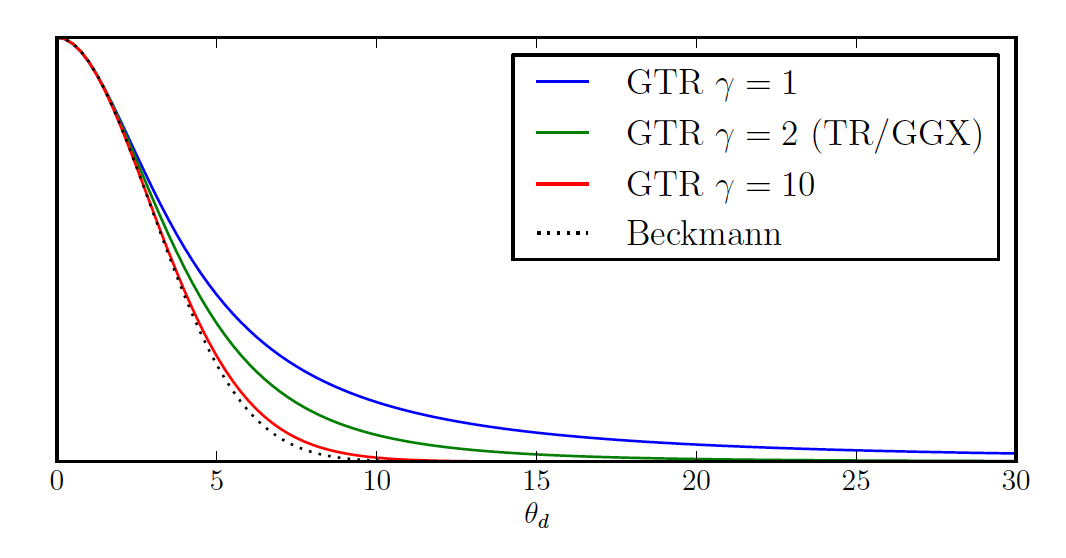
\includegraphics[scale=0.37]{gtrggx}}
    \caption{Gr\'afica de las curvas obtenidas para diferentes valores de $\gamma$}
    \vspace{0.5cm}
  \end{figure}
  \newpage
  Funci\'on de distribuci\'on de las normales en ThreeJs:\\

  \begin{equation}
    D_{GGX}(m) = \frac{\alpha^2}{\pi((n\cdotp{m})^2(\alpha^2 - 1 ) + 1)^2}
  \end{equation}
  \singlespacing

  Funci\'on de distribuci\'on de las normales en Disney 2012:\\

  \begin{equation}
    D_{GTR} = \frac
    {c}
    {(\alpha^2 cos^2 \theta_h + sin^2 \theta_h)^2}
  \end{equation}
  \singlespacing

  \begin{lstlisting}[caption=Implementaci\'on en ThreeJs del t\'ermino de geometr\'ia]
float D_GGX( const in float alpha, const in float dotNH ) {

  float a2 = pow2( alpha );
  float denom = pow2( dotNH ) * ( a2 - 1.0 ) + 1.0;

  return RECIPROCAL_PI * a2 / pow2( denom );
}
  \end{lstlisting}
  \singlespacing

  \subsection*{T\'ermino F}
  Igual que en el modelo de Disney 2012, se considera la funci\'on de Fresnel-Schlick lo suficientemente precisa para
  estimar el Fresnel, sin embargo, en \'este caso se utiliza la aproximaci\'on presentada por Epic en el Siggraph de 2013 \autocite{unreal}.\\

  \begin{equation}
    F= F_0 + (1 - F_0)2^{(-5.55473cos\theta_d - 5.55473cos\theta_d)}
  \end{equation}

  \begin{lstlisting}[caption=Implementaci\'on en ThreeJs de la aproximaci\'on a la funci\'on de Fresnel]
vec3 F_Schlick( const in vec3 specularColor, const in float dotLH ) {

  float fresnel = exp2( ( -5.55473 * dotLH - 6.98316 ) * dotLH );

  return ( 1.0 - specularColor ) * fresnel + specularColor;

}
  \end{lstlisting}

  \subsection*{T\'ermino G}
  Para definir las microfacetas en sombra o enmascaradas, ThreeJs utiliza el mismo t\'ermino que Disney 2012, usa
  la formulaci\'on de Smith para separar la funci\'on en dos componentes, luz y vista, utilizando la misma ecuaci\'on
  para las dos.\\

  $$
  V(w_i, w_o) = \frac{0.5}{V_1(w_i) + V_1(w_o)}
  $$
  \singlespacing
  \begin{equation}
    V_1(w_i) = (n \cdot{w_o}) \sqrt{((-n\cdot{w_i}) \alpha^2 + n\cdot{w_i}) n\cdot{w_i} + \alpha^2}
  \end{equation}



\begin{lstlisting}[caption=Clase MeshClothMaterial]
float G_GGX_SmithCorrelated(
  const in float alpha,
  const in float dotNL,
  const in float dotNV
) {

  float a2 = pow2( alpha );

  float gv = dotNL * sqrt( a2 + ( 1.0 - a2 ) * pow2( dotNV ) );
  float gl = dotNV * sqrt( a2 + ( 1.0 - a2 ) * pow2( dotNL ) );

  return 0.5 / max( gv + gl, EPSILON );

}
\end{lstlisting}

  \subsection*{\textit{Clearcoat}}
  El efecto de \textit{clearcoat}, se utiliza para simular efectos de barniz o recubrimientos, y se aplican tanto en Disney
  2012 como un l\'obulo secundario. Mientras que en ThreeJs se utiliza el mismo BRDF con la misma parametrizaci\'on que para
  el l\'obulo primario, en Disney 2012, var\'ia la parametrizaci\'on de los t\'erminos D y G.\\

  $$
  G_{GGX}(v) = \frac
  {2 (n \cdot{v})}
  {(n \cdot{v}) + \sqrt{ \alpha^2 + (1 - \alpha)^2 (n \cdot{v})^2 }}
  $$
  \begin{eqfloat}[!htb]
    \begin{equation}
    \textrm{siendo}\ \alpha=0.25,\;
    G_{GGX}(v) = \frac
    {2 (n \cdot{v})}
    {(n \cdot{v}) + \sqrt{ 0.0625 + 0.5625 (n \cdot{v})^2 }}
    \end{equation}
  \caption{Funci\'on de geometr\'ia para el l\'obulo de \textit{clearcoat} en ThreeJs}
  \end{eqfloat}
  \singlespacing

  \begin{lstlisting}[caption={Implementaci\'on del l\'obulo de \textit{clearcoat} en ThreeJs}]
void RE_Direct_Physical(
  const in IncidentLight directLight,
  const in GeometricContext geometry,
  const in PhysicalMaterial material,
  inout ReflectedLight reflectedLight
) {

  //...
  #ifdef CLEARCOAT

    // ...
    reflectedLight.directSpecular += ccIrradiance * material.clearcoat
      * BRDF_Specular_GGX(
        directLight,
        geometry.viewDir,
        geometry.clearcoatNormal,
        vec3( DEFAULT_SPECULAR_COEFFICIENT ),
        material.clearcoatRoughness
      );

  #else
  // ...

}
  \end{lstlisting}
  
  \subsection*{\textit{Sheen}}
  El par\'ametro de \textit{sheen} ofrece un mayor control sobre la reflectancia especular, permitiendo crear materiales con
  especulares en dos tonos.\\

  ThreeJs utiliza un BRDF diferente cuando el par\'ametro de \textit{sheen}, mientras que en el modelo de Disney el \textit{sheen}
  se modela como otro l\'obulo adicional adem\'as del de \textit{clearcoat}.\\

  Modelo de BRDF utilizando \textit{sheen} en ThreeJs: \\

  $$
  f(\textit{sheen}, \theta_d) =\frac{D_{Charlie}}{4(n\cdot{l} + n\cdot{v} - (n\cdot{l})(n\cdot{v}) )}
  $$
  \begin{equation}
    \textrm{siendo}\ D_{Charlie}(\alpha) = \frac
    {(2 + \frac{1}{\alpha})sin(\theta)^\frac{1}{\alpha}}
    {2\pi}
  \end{equation}
  \singlespacing

  L\'obulo adicional de \textit{sheen} en Disney 2012:\\

  \begin{equation}
    f(\textit{sheen}, \theta_d) = \textit{sheen} * ((1 - \textit{sheenTint}) + \textit{sheenTint} * \textit{tint}) * (1 - \cos\theta_d)^5
  \end{equation}
  \singlespacing

  \begin{lstlisting}[caption={BRDF del modelo de \textit{sheen} de ThreeJs}]
vec3 BRDF_Specular_Sheen(
  const in float roughness,
  const in vec3 L,
  const in GeometricContext geometry,
  vec3 specularColor
) {

  vec3 N = geometry.normal;
  vec3 V = geometry.viewDir;

  vec3 H = normalize( V + L );
  float dotNH = saturate( dot( N, H ) );

  return specularColor * D_Charlie( roughness, dotNH )
    * V_Neubelt( dot(N, V), dot(N, L) );

}
  \end{lstlisting}
      \chapter{Modelos de iluminaci\'on para tejidos}
% Los materiales PBR \textit{MeshStandardMaterial} y \textit{MeshPhysicalMaterial} de ThreeJs funcionan muy bien para gran parte de
% materiales, como pl\'asticos o metales. Sin embargo carecen de par\'ametros que permitan representar fen\'onmenos como la
% dispersi\'on hacia delante y hacia detr\'as (\textit{forward/backward scattering}) o la absorci\'on y reflexi\'on interna (\textit{suburface scattering}) caracter\'isticos
% de gran cantidad de tejidos debido a la reflexi\'on de la luz con las fibras que lo componen.
Los tejidos se componen de fibras entrelazadas con cierta separaci\'on entre s\'i, por lo que la met\'afora de la
rejilla compuesta por microespejos que se utiliza en la teor\'ia de microfacetas no es la mejor aproximaci\'on para tratar
de representar este material de forma realista. Los materiales PBR \textit{MeshStandardMaterial} y \textit{MeshPhysicalMaterial} de
ThreeJs, basados en microfacetas, funcionan muy bien para gran parte de materiales, como pl\'asticos o metales, sin embargo no consiguen
una representaci\'on realista de tejidos, que suelen presentar un l\'obulo especular m\'as atenuado.\\

% La estructura de fibras puede provocar los efectos de absorci\'on y reflexi\'on interna (\textit{subsurface scattering}) y, dependiendo
% de la direcci\'on de la luz, los efectos de dispesi\'on hacia delante o hacia detr\'as (\textit{forward} y \textit{backward scattering}).
% Cuando la luz viene en direcci\'on opuesta al punto de vista y golpea las fibras que salen del tejido provoca el efecto de
% \textit{foward scattering}, mientras que cuando la luz viene en la misma direcci\'on que el punto de vista, el fen\'omeno
% de \textit{backward scattering}. El terciopelo es un caso de tejido en el que se acent\'ua este efecto y el primer trabajo en describirlo, el modelo de BRDF de Ashikmin
% \autocite{ashikhmin}, es tambi\'en conocido como \textit{velvet BRDF} o \textit{velvet distribution}.\\
La estructura de fibras puede provocar los efectos de absorci\'on y reflexi\'on interna (\textit{subsurface scattering}) y, dependiendo
de la direcci\'on de la luz, o los efectos de dispesi\'on hacia delante ((\textit{forward scattering}) que se produce cuando la luz viene
en direcci\'on opuesta al punto de vista y golpea las fibras que salen del tejido, o la dispersi\'on hacia detr\'as (\textit{backward scattering}),
cuando la luz viene en direcci\'on opuesta al punto de vista. El terciopelo es un caso de tejido en el que se acent\'ua este efecto y el primer
trabajo en describirlo, el modelo de BRDF de Ashikmin \autocite{ashikhmin}, es tambi\'en conocido como \textit{velvet BRDF} o
\textit{velvet distribution}.\\


Este trabajo implementa sobre ThreeJs el modelo de \textit{Cloth} de Filament \autocite{filament}. La librer\'ia de Google
presenta un BRDF especial para tejidos que, inspirado en los trabajos de Ashikmin \autocite{ashikhmin} y m\'as
tarde Estevez y Kulla \autocite{sheenbrdf} para el t\'ermino de distribuci\'on de las normales, y el de Neubelt \autocite{theorder}
para el factor de geometr\'ia, permite una representaci\'on realista en entornos interactivos de los efectos mencionados.

% al carecer de par\'ametros que permitan representar los fen\'onmenos de dispersi\'on hacia delante y hacia detr\'as (\textit{forward/backward scattering})
% o la absorci\'on y reflexi\'on interna (\textit{suburface scattering}), efectos caracter\'isticos de una amplia variedad de
% tejidos.\\

% Dependiendo de la direcci\'on de la luz con respecto al punto de vista, las fibras que componen los tejidos pueden provocar los
% efectos de \textit{forward scattering} cuando la luz viene de la direcci\'on opuesta al punto de vista y  \textit{backward scattering},
% cuando la luz viene desde la misma direcci\'on que el punto de vista. 

% Adem\'as la separaci\'on de las fibras puede 

% Adem\'as las ligeras separaciones


% los fen\'omenos de retrodispersi\'on o
% la reflexi\'on interna, compuestos de una gran cantidad de hilos que absorben y dispersan la luz.
% Es por ello que Filament presenta un nuevo BRDF basado en los trabajos de y que utiliza un par\'ametro de \textit{sheen} para
% que ofrece un control sobre el brillo especular para simular los fen\'omenos de reflexi\'on hacia delante y hacia detr\'as
% caracter\'istico de tejidos como el terciopelo. Adem\'as algunos materiales absorben parcialmente la luz y la emiten de nuevo,
% aport\'ando un color caracter\'istico determinado por las fibras del tejido, \'este fen\'omeno se representa con el par\'ametro
% \textit{subsurface} de Filament, que utiliza la aproximaci\'on conocida como \textit{wrapped diffuse lighting} \autocite{gpugems}\\


\section{Integraci\'on de una nueva clase de material en ThreeJs}
ThreeJs ofrece la posibilidad de crear materiales a trav\'es de su API, sin embargo, para este trabajo se ha decidido
crear un \textit{fork} de la librer\'ia para soportar posibles nuevos materiales y funcionalidades que se requieran
espec\'ificamente de Author.\\

En este cap\'itulo se explica la implementaci\'on de una nueva clase de material que se integra en la librer\'ia de materiales
de ThreeJs. Siguiendo la nomenclatura de la librer\'ia (\textit{MeshBasicMaterial}, \textit{MeshStandardMaterial}, etc.), el
nuevo material se llamar\'a \textit{MeshClothMaterial}.


% ThreeJs proporciona una API para extender de forma sencilla su librer\'ia de materiales, sin embargo, para proporcionar al nuevo
% material de la misma interfaz que los materiales nativos de ThreeJs, as\'i como seguir extendiendo la librer\'ia y ser flexible
% a futuros cambios, se ha optado por crear un \textit{fork} de la librer\'ia e introducir los cambios necesarios para crear
% este nuevo material.\\

% Siguiendo la nomenclatura de ThreeJs: \textit{MeshBasicMaterial}, \textit{MeshStandardMaterial}, etc., el nuevo material se
% llama \textit{MeshClothMaterial}.\\

\begin{figure}[H]
  \centering
    \frame{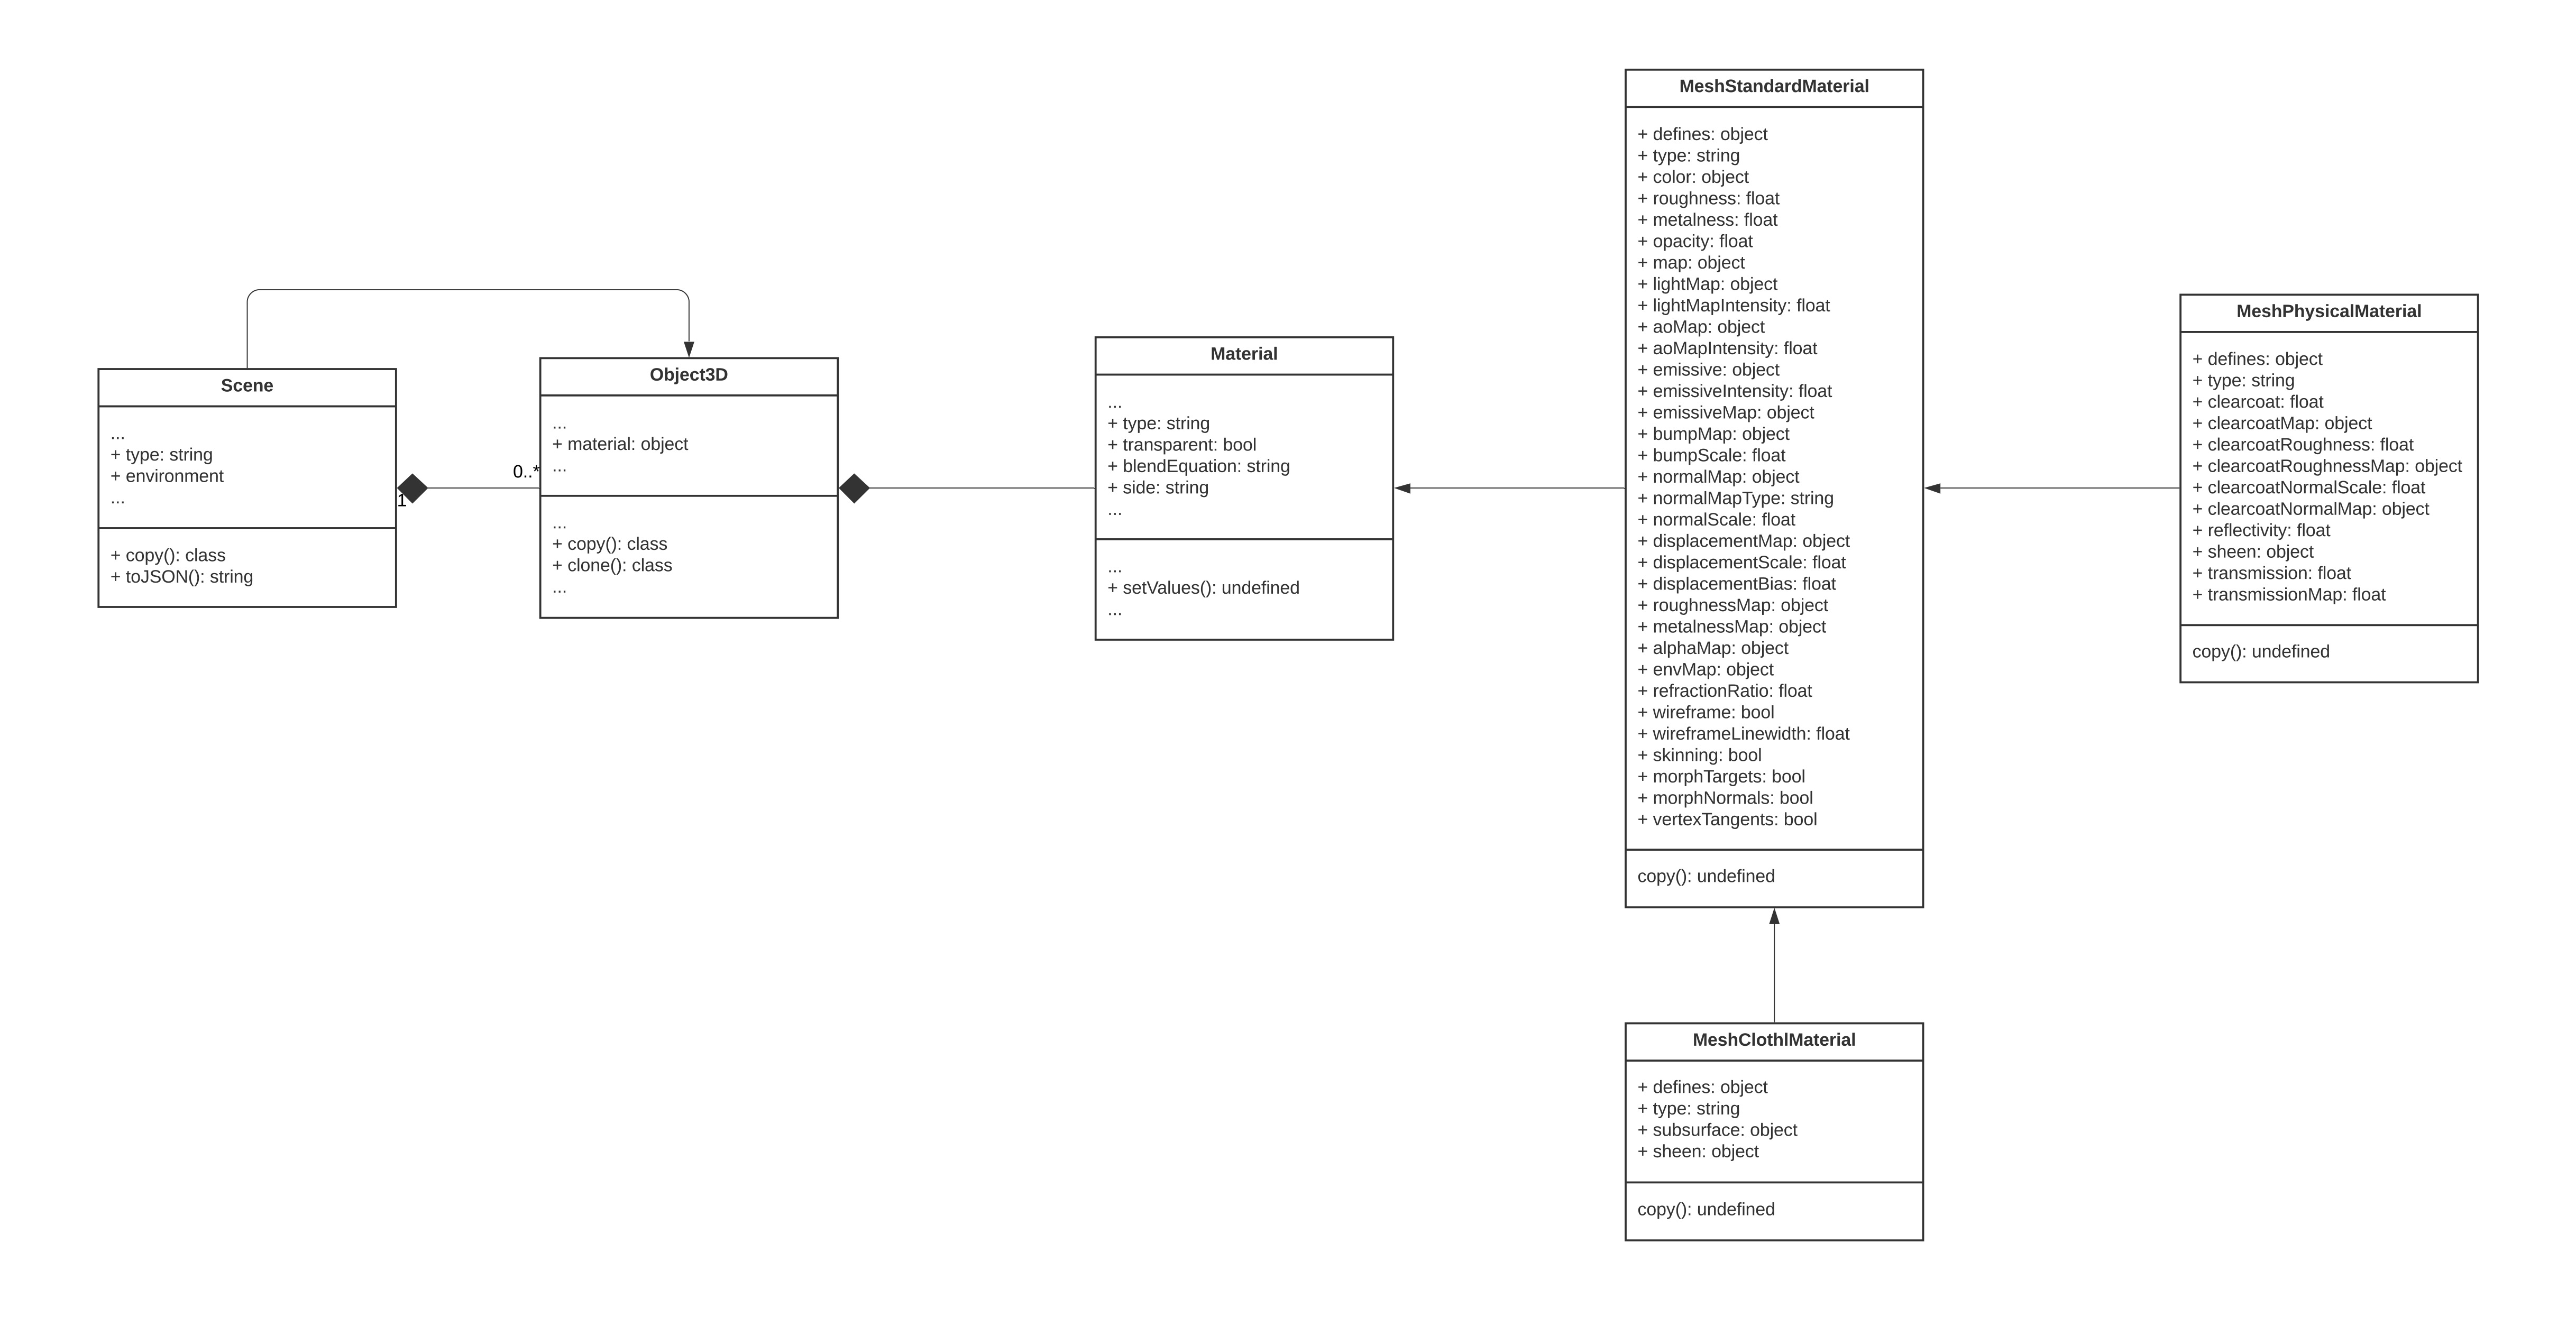
\includegraphics[scale=0.35]{threejs_meshcloth_integration_material}}
  \caption{Integraci\'on de la nueva clase \textit{MeshClothMaterial}}
\end{figure}
\singlespacing

El nuevo material tiene un BRDF diferente al \textit{MeshPhysicalMaterial},
y diferentes par\'ametros, sin embargo soporta los mismos efectos de \textit{normal mapping}, \textit{displacement}, etc.
y comparte gran cantidad de los par\'ametros con el material base, a\~nadiendo \textit{subsurface}, \textit{sheen}.
\textit{MeshClothMaterial} utiliza sus propios \textit{type}, para identificar el tipo de shader, en la clase \textit{WebGLMaterials}
y \textit{defines}, que se utilizar\'an para a\~nadir directivas de preprocesador al c\'odigo GLSL generado en la clase
\textit{WebGLProgram}. Para que el nuevo material est\'e quede expuesto como un material nativo de ThreeJs,
se an\~ade a objeto \textit{Materials}.

\begin{figure}[H]
  \vspace{0.5cm}
  \centering
    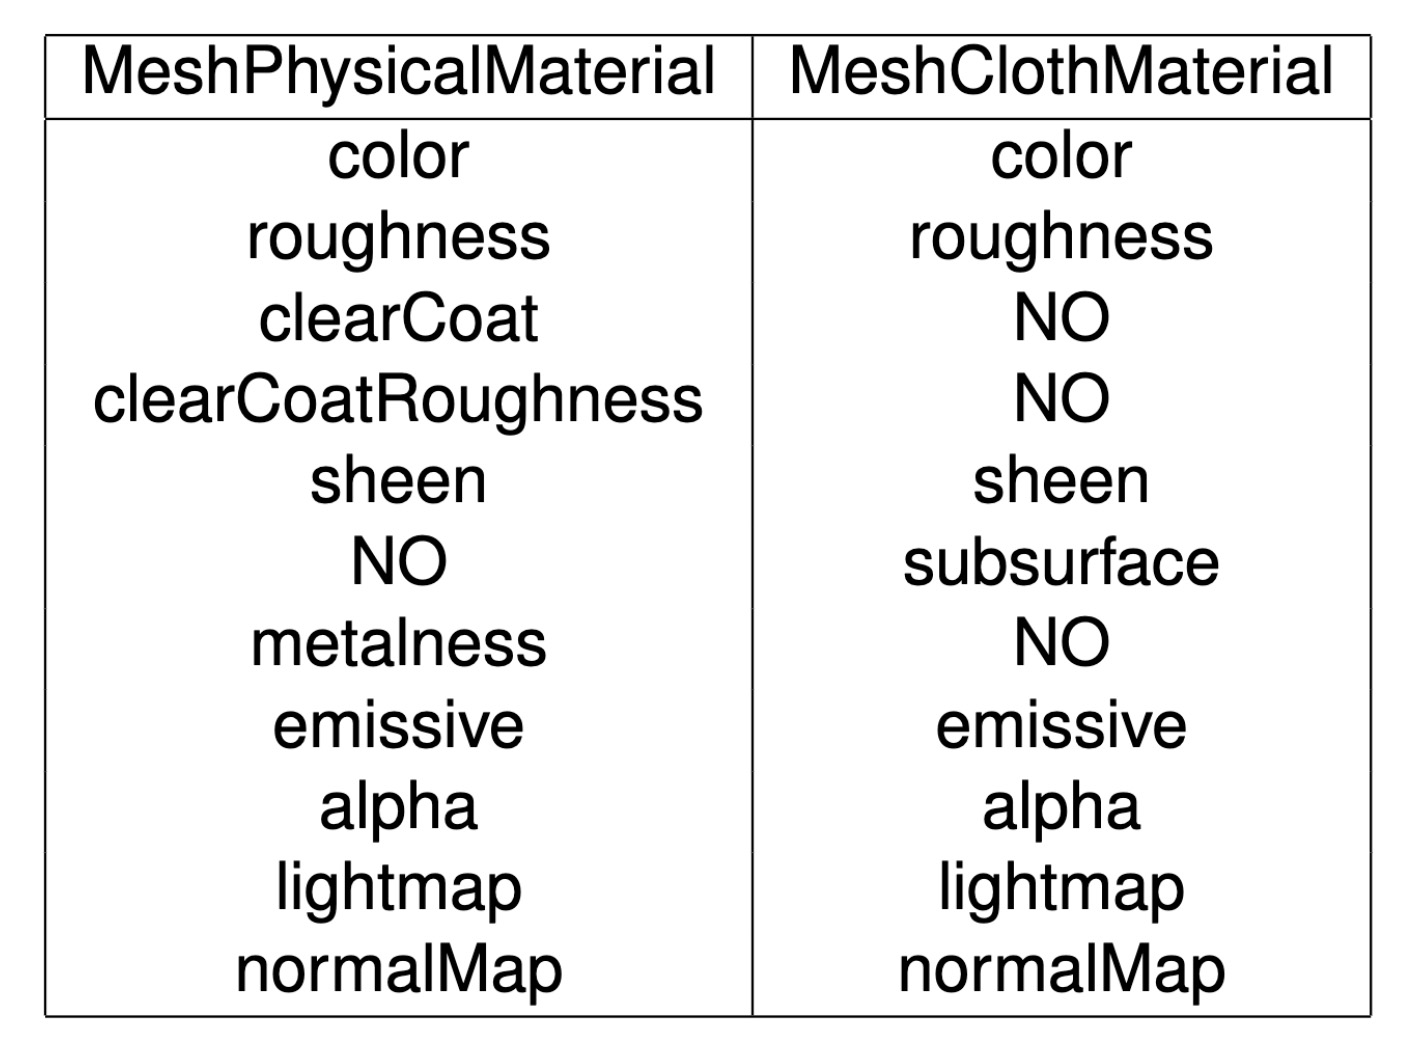
\includegraphics[scale=0.34]{comparison_physical_cloth}
  \caption{Comparativa \textit{MeshPhysicalMaterial}, \textit{MeshClothMaterial}}
  \vspace{0.5cm}
\end{figure}


En la clase \textit{WebGLMaterials} se incluye un nuevo m\'etodo para actualizar los uniforms de \'este nuevo material.\\

\singlespacing
\begin{lstlisting}[caption=Cambios sobre la clase WebGLMaterials de ThreeJs]
// WebGLMaterials.js

// ...
refreshUniformsCommon( uniforms, material );
// ...
function refreshUniformsCloth( uniforms, material, environment ) {

  refreshUniformsStandard( uniforms, material, environment );

  uniforms.reflectivity.value = material.reflectivity; // also part of uniforms common

  if ( material.sheen ) {

    uniforms.sheen.value.copy( material.sheen );

  } else {

    uniforms.sheen.value.copy( material.color );
    uniforms.sheen.value.r = Math.sqrt( uniforms.sheen.value.r );
    uniforms.sheen.value.g = Math.sqrt( uniforms.sheen.value.g );
    uniforms.sheen.value.b = Math.sqrt( uniforms.sheen.value.b );

  }

  if ( material.subsurface ) {
    uniforms.subsurface.value.copy( material.subsurface );
  }

  if ( material.brdfCloth ) {
    uniforms.brdfCloth.value = material.brdfCloth;
  }
}
// ...
\end{lstlisting}
\singlespacing

En la clase \textit{WebGLProgram} se modifica el constructor para para a\~nadir las directivas de precompilaci\'on
para los par\'ametros \textit{subsurface} y \textit{sheen}, en caso de utilizarse estos par\'ametros.\\

\begin{lstlisting}[caption=Cambios sobre la clase WebGLProgram de ThreeJs]
// WebGLProgram.js
// ...
function WebGLProgram( renderer, cacheKey, parameters, bindingStates ) {
  // ...
  prefixFragment = [
    // ...
    ( parameters.sheen || parameters.shaderID === 'cloth' ) ? '#define USE_SHEEN' : '',
    parameters.subsurface ? '#define SUBSURFACE' : '',
    // ...
  ]
  // ...
}
// ...
\end{lstlisting}
\singlespacing

En el closure \textit{WebGLPrograms} se actualiza an\~ade una clave para el nuevo tipo de material, \textit{MeshClothMaterial}
y se a\~nade la cadena de texto \textit{subsurface} al array \textit{parameterNames}, adem\'as de a\~nadir nuevas claves para
el \textit{subsurface} y la informaci\'on precomputada del BRDF, dentro del objeto \textit{parameters} dentro de la funci\'on
\textit{getParameters}. De esta forma nos aseguramos que el sistema interpreta correctamente el nuevo material y puede acceder
y cachear sus propiedades.

\singlespacing
\begin{lstlisting}[caption=Cambios sobre la clase WebGLPrograms de ThreeJs]
// WebGLPrograms.js
// ...
const shaderIDs = {
  // ...
  MeshClothMaterial: 'cloth',
  // ...
};

const parameterNames = [
  // ...
  "subsurface", "brdfCloth",
  // ...
];
// ...
function getParameters( material, lights, shadows, scene, object ) {
  // ...
  const parameters = {
    // ...
    subsurface: !! material.subsurface,
    brdfCloth: !! envMap && shaderID === 'MeshClothMaterial',
    // ...
  };
  // ...
}
// ...
\end{lstlisting}


% ThreeJs utiliza un sistema de chunks (trozos) se componen en tiempo de ejecuci\'on para acabar formando los vertex
% y fragment shaders que se utilizan en los programas de WebGL. Los chunks se componen en la libreria de shaders, la
% clase ShaderLib.
% Para crear nuestro MeshClothMaterial, hemos de extender de la clase base Material, de la que extienden el resto de
% materiales. En este caso, de la misma forma que hace MeshPhysicalMaterial, extenderemos de MeshStandardMaterial,
% que dispone de la mayor parte de uniforms y attributes que necesita nuestro shader.\\

% Para que el motor de render de ThreeJs reconozca este nuevo material es necesario, a\~nadir
% su tipo (MeshClothMaterial) al mapa de ShaderIds para que el gestor de programas (WebGLPrograms)
% lo utilice para detectar obtener los uniforms y shaders necesarios para el material. Adem\'as
% los nuevos par\'ametros necesarios para el material se deben de incluir en el array
% parametersNames, de forma que el sistema de cacheo de programas de ThreeJs detecte estas
% nuevas propiedades.\\

% Finalmente, en el gestor de materiales de ThreeJs, necesitamos a\~nadir un nuevo m\'etodo
% que actualice los unfiroms del programa creado, de la misma forma que se hace con los
% materiales nativos de la librer\'ia.\\

% De esta forma, tenemos un material con la interfaz nativa de ThreeJs, que tiene acceso a los
% chunks definidos en la clase ShaderChunk y cuyos uniforms y composici\'on de chunks definiremos
% en ShaderLib.\\

% El BRDF para el componente especular de la iluminaci\'on directa del material Cloth de Filament,
% se utiliza en ThreeJs para a\~nadir opcionalmente un l\'obulo de Sheen al material. Por otra
% parte, el difuso, utiliza en Filament un t\'ermino opcional para ofrecer una aproximaci\'on
% barata el subsurface scattering para iluminaci\'on directa que utiliza Filament.\\


\vspace{1cm}
\section{Integraci\'on del nuevo \textit{shader} sobre ThreeJs}
  Para a\~nadir un nuevo BRDF hemos de extender el sistema de \textit{chunks} de ThreeJs. Para ello hemos de a\~nadir el
  punto de entrada del nuevo shader al objeto \textit{shaderChunk}. Siguiendo el sistema de nomenclatura de ThreeJs,
  llamaremos \textit{meshcloth\_frag.glsl.js} al nuevo shader, que utiliza chunks comunes con el \textit{MeshStandardMaterial},
  salvo para el c\'aculo de la iluminaci\'on directa e indirecta, que utiliza sus propios \textit{chunks} para el c\'aculo
  de la ecuaci\'on de render: \textit{lights\_cloth\_fragment.glsl.js}, donde se inicializa la estructura de datos relativa
  al material y \textit{lights\_cloth\_pars\_fragment.glsl.js}, donde se calculan las ecuaciones de render de la iluminaci\'on
  directa e indirecta del nuevo material.

  \subsection{Componente difusa}
  El color difuso y el color de \textit{subsurface}, modelan en realidad el mismo fen\'omeno f\'isico, la cantidad de reflexi\'on
  interna que resulta en aportaci\'on sobre la reflexi\'on en direcci\'on al vector de vista. Cuando la distancia de reflexi\'on
  es despreciable en comparaci\'on con el tama\~no del pixel, se aproxima como una reflexi\'on difusa, sin embargo, cuando
  la distancia es considerable, el fen\'omeno se modela de forma diferente.\\
  
  En tiempo real, es com\'un utilizar la citada aproximaci\'on 
  El modelo para tejidos de Filament utiliza el difuso de Lambert en caso de no utilizar el par\'ametro \textit{subsurface},
  mientras que si lo utiliza utiliza el factor de correcci\'on de la t\'ecnica \textit{wrapped diffuse lighting} \autocite{gpugems}
  que permite aproximar el efecto debido a la absorci\'on y flexi\'on interna de la luz incidente en la superficie.\\

  \begin{eqfloat}[!htb]
    \begin{equation}
      f_d(v, h) = \frac{c_{diff}}{\pi}
      \Bigg\langle
      \frac{(n\cdot{l})w}{(1+ w)^2}( c_{subsurface} + n \cdot{l} )
      \Bigg\rangle
    \end{equation}
  \caption{Componente difusa del modelo de \textit{Cloth} en Filament}
  \end{eqfloat}

  \singlespacing
  \begin{lstlisting}[caption=Implementaci\'on del BRDF para la componente difusa de \textit{MeshClothMaterial}]
vec3 BRDF_Diffuse_Cloth(
  const in IncidentLight incidentLight,
  const in vec3 viewDir,
  const in vec3 normal,
  const in vec3 diffuseColor
) {

  float dotNL = dot( normal, incidentLight.direction );
  float radiance = RECIPROCAL_PI; // Lambert BRDF
  
  #if defined(SUBSURFACE)
    // Fd_Wrap
    radiance *= saturate((dotNL + 0.5) / 2.25);
  #endif

  vec3 Fd = radiance * diffuseColor;

  return Fd;

}

void RE_Direct_Cloth(
  const in IncidentLight directLight,
  const in GeometricContext geometry,
  const in PhysicalMaterial material,
  inout ReflectedLight reflectedLight
) {

  // ...
  reflectedLight.directDiffuse += irradiance * BRDF_Diffuse_Cloth(
    directLight,
    geometry.viewDir,
    geometry.normal,
    material.diffuseColor
  );

  #if defined(SUBSURFACE)
    reflectedLight.directDiffuse *= saturate(subsurface + dotNL); 
  #endif
  // ...

}
  \end{lstlisting}


  \subsection{Componente especular}

  El \textit{MeshPhysicalMaterial} utiliza por defecto un BRDF GGX, \autocite{ggx}. Sin embargo, si el par\'ametro de \text{sheen}
  est\'a activo, utiliza 
  Al contrario que el MeshPhysicalMaterial, que utiliza una una distribucion GGX, el material
  Cloth de Filament utiliza una  version modificada del BRDF presentado por Ashikmin y Premoze.
  \autocite{ashikhmin}\\

  \begin{eqfloat}[!htb]
    \begin{equation}
      D_{Velvet}(v, h, \alpha) = c_{norm} (
        1 + 4exp \left(\frac{-cot^2\theta_h}{\alpha^2}\right)
      )
    \end{equation}
  \caption{\textit{Velvet distribution} \autocite{ashikhmin}}
  \end{eqfloat}

  \begin{eqfloat}[!htb]
    \begin{equation}
      D_{Charlie}(\alpha) = \frac
      {(2 + \frac{1}{\alpha})sin(\theta)^\frac{1}{\alpha}}
      {2\pi}
    \end{equation}
  \caption{Componente difusa del modelo de \textit{Cloth} en Filament}
  \end{eqfloat}
  \singlespacing

  \begin{lstlisting}[caption=Implementaci\'on del factor de distribuci\'on de Charlie en ThreeJs]
float D_Charlie(float roughness, float NoH) {
  // Estevez and Kulla 2017, "Production Friendly Microfacet Sheen BRDF"
  float invAlpha = 1.0 / roughness;
  float cos2h = NoH * NoH;
  float sin2h = max(1.0 - cos2h, 0.0078125); // 2^(-14/2), so sin2h^2 > 0
                                             // in fp16
  return (2.0 + invAlpha) * pow(sin2h, invAlpha * 0.5) / (2.0 * PI);
}
  \end{lstlisting}
  \singlespacing

  Mientras que para el factor de geometr\'ia o visibilidad se utiliza la version modificada de Neubelt \autocite{theorder}
  del denominador de microfacetas para suavizar el degradado de la sombra.

  \begin{eqfloat}[!htb]
    \begin{equation}
      \frac{1}{4(n\cdot{l} + n\cdot{v} - (n\cdot{l})(n\cdot{v}) )}
    \end{equation}
  \caption{Formulaci\'on del t\'ermino de geometr\'ia de Neubelt \autocite{theorder}}
  \end{eqfloat}

  \begin{lstlisting}[caption=Implementaci\'on del t\'ermino de de visibilidad de Neubelt \autocite{theorder}]
float V_Neubelt(float NoV, float NoL) {
  // Neubelt and Pettineo 2013, "Crafting a Next-gen Material Pipeline for The Order: 1886"
  return saturate(1.0 / (4.0 * (NoL + NoV - NoL * NoV)));
}
  \end{lstlisting}

  \singlespacing
  \begin{lstlisting}[caption=Cambios sobre la clase WebGLPrograms de ThreeJs]
vec3 BRDF_Specular_Sheen( const in float roughness, const in vec3 L, const in GeometricContext geometry, vec3 specularColor ) {

  vec3 N = geometry.normal;
  vec3 V = geometry.viewDir;

  vec3 H = normalize( V + L );
  float dotNH = saturate( dot( N, H ) );

  return specularColor * D_Charlie( roughness, dotNH ) * V_Neubelt( dot(N, V), dot(N, L) );

}
  \end{lstlisting}

  \subsection{Iluminaci\'on indirecta}
    De las t\'ecnicas de iluminaci\'on indirecta vistas en el cap\'itulo 3, ThreeJs soporta tanto mapas de
    irradiancia como esf\'ericos harm\'onicos para la componente difusa, mientras que para la componente
    especular utiliza la aproximaci\'on anal\'itica presentada por Lazarov \autocite{blackops}.

    \subsubsection{Componente difusa}
      Para el c\'alculo del difuso, ha de estimarse la irradiancia debida al entorno sobre un punto y multiplicarlo
      por el BRDF difuso. ThreeJs soporta ambas t\'enicas vistas en el cap\'itulo 3 para el c\'alculo de irradiancia:
      mapas de irradiancia y esf\'ericos harm\'onicos.

      \begin{eqfloat}[!htb]
        \begin{equation}
          L_o(p, w_o) = k_d \frac{c}{\pi} \int_{\Omega}{L_i(p, w_i) n\cdot{w_i}dw_i}
        \end{equation}
      \caption{C\'alculo de la luz indirecta difusa}
      \end{eqfloat}

      La t\'ecnica de mapas de irradiancia, aunque muy eficiente durante la ejecuci\'on, son muy costosas como para
      ser generadas bajo demanda en un entorno interactivo. Por su parte, los esf\'ericos harm\'onicos reducen el coste
      de generacion de los mapas de entorno a costa de comprimir la informaci\'on de irradiancia en un representaci\'on
      de frecuencias frente a espacio.\\

      Los \textit{chunks} de ThreeJs separan el c\'aculo de la luz indirecta en una funci\'on para cada componente, difuso
      y especular. El c\'aculo de la componente difusa se realiza en la funci\'on \textit{RE\_IndirectDiffuse\_Cloth}.\\

      \begin{lstlisting}[caption=C\'alculo de la ecuaci\'on de render para la componente difusa de \textit{MeshClothMaterial}]
  void RE_IndirectDiffuse_Cloth( const in vec3 irradiance, const in GeometricContext geometry, const in PhysicalMaterial material, inout ReflectedLight reflectedLight ) {
  
      reflectedLight.indirectDiffuse += irradiance * BRDF_Diffuse_Lambert( material.diffuseColor );
  
  }
      \end{lstlisting}

      Sin embargo, para tener en cuenta el principio de conservaci\'on de la energ\'ia, $k_d + k_s = 1$, tal y como se
      presenta en el modelo de Cook-Torrance \autocite{cooktorrance}, parte del c\'alculo se hace en la funci\'on
      \textit{RE\_IndirectSpecular\_Cloth}, que eval\'ua la componente especuar. \textit{RE\_IndirectSpecular\_Cloth}
      utiliza un mapa prefiltrado de entorno, explicado en el cap\'itulo 3, para calcular la irradiancia, que se le resta al
      total de energ\'ia (1), para obtener el peso de la irradiancia difusa. Finalmente, en caso de utilizar \textit{subsurface},
      se aplica el factor de correcci\'on.\\



      % ThreeJs utiliza dos enfoques, por una parte, mapas de irradiancia y por otra, light probes, que
      % utilizan spherical harmonics. Los mapas de irradiancia son una tecnica IBL (Image Based Lighting)
      % tratan todo el entorno como una fuente de luz y utilizan im\'agenes precomputadas que permiten
      % acelerar este calculo.\\

      % La parte integral de la ecuaci\'on se resuelve utilizando el mapa de irradiancia,
      % que utiliza un factor de correci\'on en caso de estar modelando la refracci\'on interna,

      \begin{lstlisting}
void RE_IndirectSpecular_Cloth(
  const in vec3 radiance,
  const in vec3 irradiance,
  const in vec3 clearcoatRadiance,
  const in GeometricContext geometry,
  const in PhysicalMaterial material,
  inout ReflectedLight reflectedLight
) {
  // ...

  float diffuseWrapFactor = 1.0;
  #if defined(SUBSURFACE)
    diffuseWrapFactor *= saturate(
      (dotNV + subsurfaceIntensity)
      / ((1.0 + subsurfaceIntensity) * (1.0 + subsurfaceIntensity))
    );
  #endif

  // E = specular irradiance
  vec3 FdSH = reflectedLight.indirectDiffuse * ( 1.0 - E )
    * diffuseWrapFactor;
  vec3 FdIM = irradiance * BRDF_Diffuse_Lambert( material.diffuseColor )
    * ( 1.0 - E ) * diffuseWrapFactor;

  vec3 Fd = Fd_SH + Fd_Lod;

  #if defined(SUBSURFACE)

    Fd *= saturate(subsurface + dotNV);

  #endif
  // ...

  reflectedLight.indirectDiffuse = Fd;

}
      \end{lstlisting}

      \singlespacing

    \subsubsection{Componente especular}
      Tanto ThreeJs utilizan la t\'ecnica \textit{split-sum approximation} \autocite{dfgapproximation}
      en la componente especular. Sin embargo, mientras que Filament utiliza un \textit{BRDF integration map},
      ThreeJs utiliza la aproximaci\'on presentada por Epic \autocite{dfgapproximation}, ambas presentadas en
      el cap\'itulo 3.\\

      \begin{eqfloat}[ht]
        \begin{equation}
          \resizebox{0.95\hsize}{!}{%
          $L_o(p, w_o) =
          \int_{\Omega} k_s \frac{DFG}{4(w_o\cdot{n})(w_i\cdot{n})})L_i(p, w_i)n\cdot{w_i}dw_i = \\
          \int_{\Omega} k_s \frac{DFG}{4(w_o\cdot{n})(w_i\cdot{n})}) *
          \int_{\Omega}L_i(p, w_i)n\cdot{w_i}dw_i$   
          }
        \end{equation}
      \caption{Separaci\'on de la integral de la componente especular en la integral del BRDF y la integral de la radiancia }
      \end{eqfloat}
      
      La aproximaci\'on de ThreeJs del BRDF especular funciona especialmente bien para dispositivos con un rendimiento
      limitado. Esta aproximaci\'on de la integral del BRDF es una soluci\'on anal\'itica para el BRDF GGX \autocite{ggx},
      por lo que no es correcta para el nuevo BRDF del modelo de telas.\\

      \begin{lstlisting}[caption=Apromixaci\'on anal\'itica a la integral del BRDF en ThreeJs]
        vec2 integrateSpecularBRDF( const in float dotNV, const in float roughness ) {
          const vec4 c0 = vec4( - 1, - 0.0275, - 0.572, 0.022 );
          const vec4 c1 = vec4( 1, 0.0425, 1.04, - 0.04 );
          vec4 r = roughness * c0 + c1;
          float a004 = min( r.x * r.x, exp2( - 9.28 * dotNV ) ) * r.x + r.y;
          return vec2( -1.04, 1.04 ) * a004 + r.zw;
        }
      \end{lstlisting}
      \singlespacing
      

      El nuevo modelo de telas, de la misma forma que Filament, utiliza un \textit{BRDF integration map} para almacenar
      en los canales rojo y azul la escala y offset del Fresnel para el modelo GGX \autocite{ggx}. El resultado del BRDF de tejidos,
      que no utiliza Fresnel, se almacena en el canal azul, al que se accede de igual forma que al \textit{BRDF integration map} para el modelo GGX \autocite{ggx},
      utilizando $n\cdot{l}$ para el eje $x$ y el valor de rugosidad del material para el eje $y$.

      % Mientras que Filament utiliza un 

      % Para el especular, la 
      % \autocite{blackops}. \'Esta t\'ecnica permite separar la en dos partes la soluci\'on de la
      % integral.

      % Por una parte, el mapa prefiltrado de entorno es un mapa preconvolucionado que tiene en cuenta
      % los posibles valores de rugosidad del material de forma que a medida que el ruido es mayor, las
      % reflexiones son de un color menos definido. Esta tecnica utiliza simplifica el calculo de
      % la integral asumiendo la direccion de la vista igual a la direccion de sampleo.\\

      % Por otra parte, el c\'alculo del BRDF se almacena en una textura, conocida como mapa de integral
      % del BRDF, utilizando $n\cdot{w_i}$ en el eje $x$ y $roughness$ en el eje y.

      \begin{figure}[H]
        \vspace{0.5cm}
        \centering
          \frame{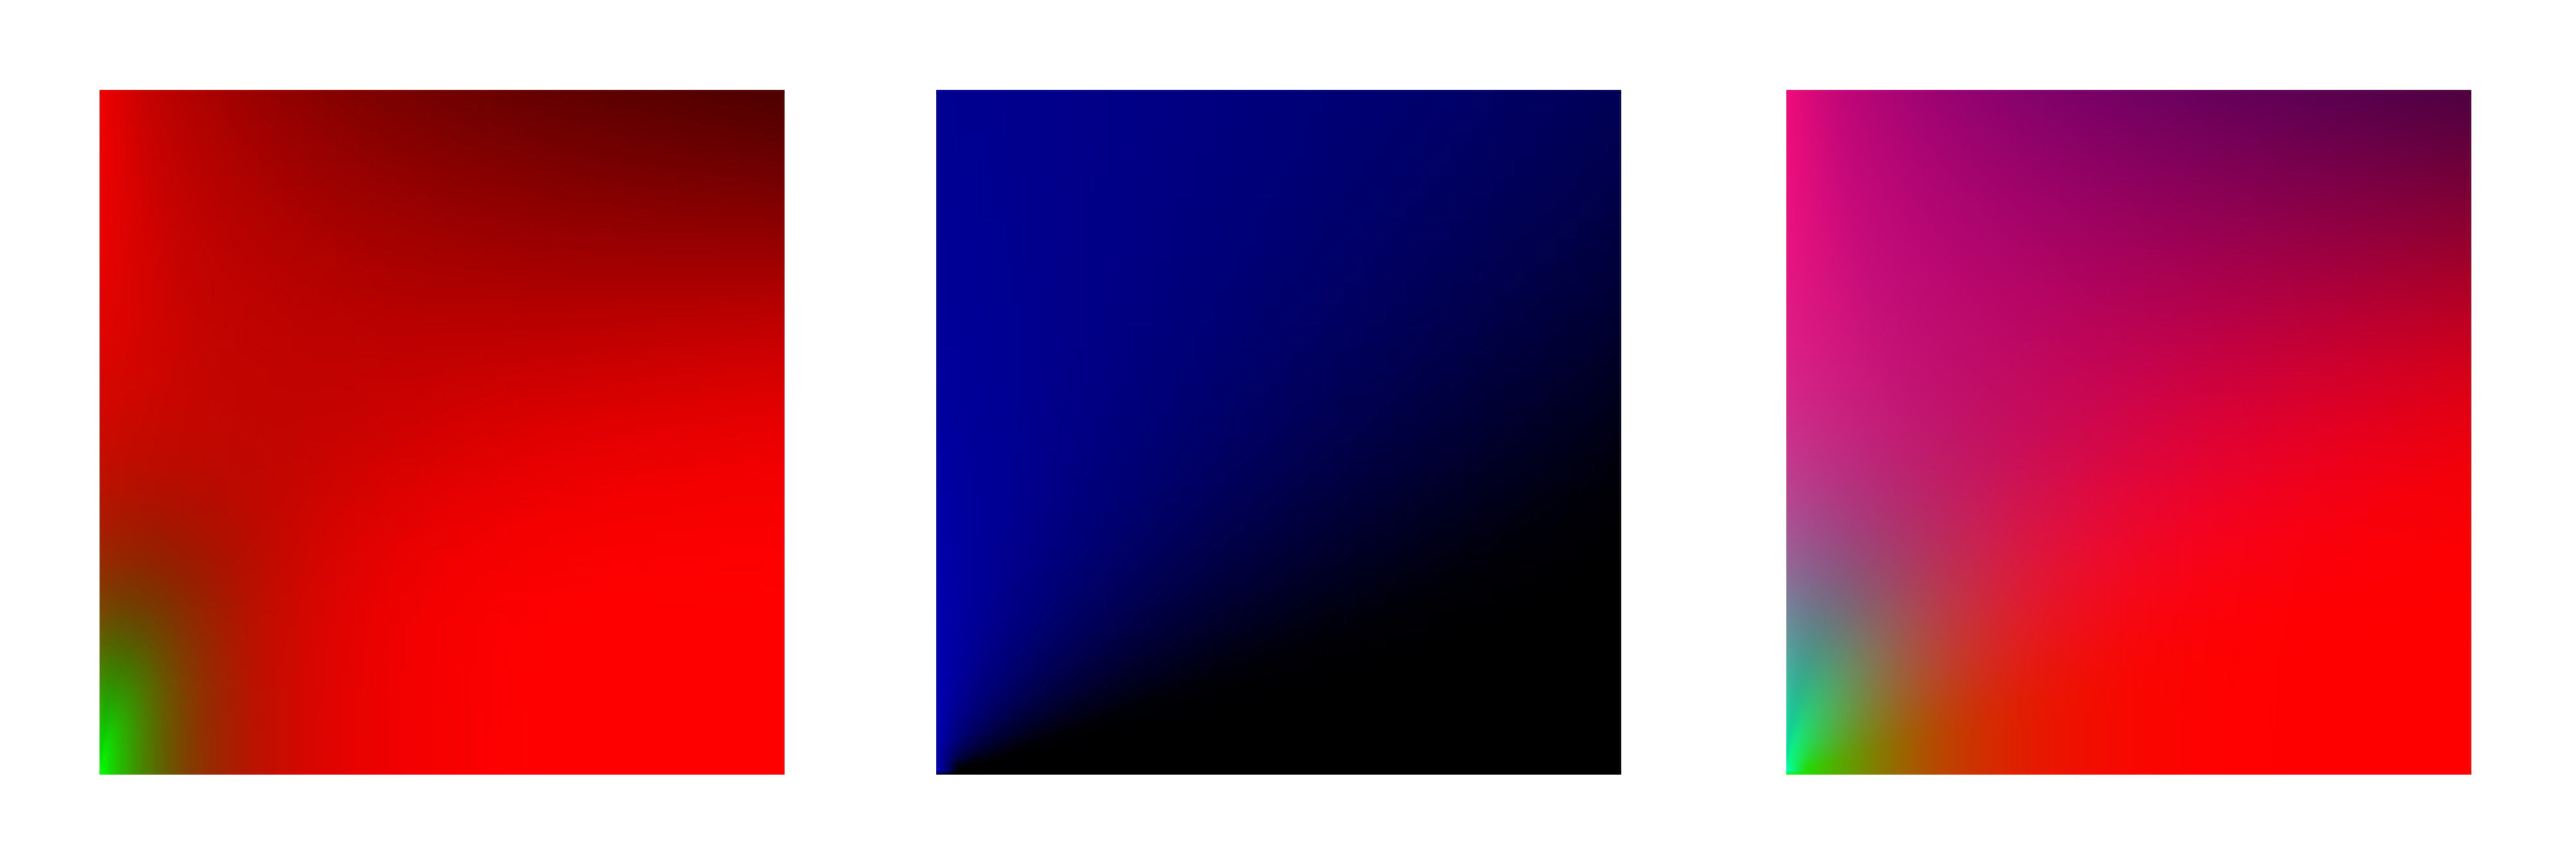
\includegraphics[scale=0.35]{splitsumcloth}}
        \caption{Canales RG (BRDF GGX \autocite{ggx}), B (BRDF para telas \autocite{filament}) y la suma de ellos,
        RGB, del \textit{BRDF integration map}}
        \vspace{0.5cm}
      \end{figure}

    \begin{lstlisting}[caption=C\'alculo de la irradiancia del entorno para el modelo de telas utilizando el nuevo \textit{BRDF integration map}]
float prefilteredDG = textureLod(
  brdfCloth,
  vec2( dotNV, material.specularRoughness * material.specularRoughness ),
  0.0
).b;

vec3 E = material.sheenColor * prefilteredDG;
reflectedLight.indirectSpecular += E * radiance;
    \end{lstlisting}
    \singlespacing

    \begin{lstlisting}[caption=C\'alculo de iluminaci\'on indirecta de \textit{MeshClothMaterial}]
void RE_IndirectSpecular_Cloth(
  const in vec3 radiance,
  const in vec3 irradiance,
  const in vec3 clearcoatRadiance,
  const in GeometricContext geometry,
  const in PhysicalMaterial material,
  inout ReflectedLight reflectedLight
) {

  float dotNV = dot( geometry.normal, geometry.viewDir );

  float prefilteredDG = textureLod(
    brdfCloth,
    vec2(
      dotNV,
      material.specularRoughness * material.specularRoughness
    ),
    0.0
  ).b;

  vec3 E = material.sheenColor * prefilteredDG;
  reflectedLight.indirectSpecular += E * radiance;

  // ...

}
    \end{lstlisting}
    \singlespacing

Como res\'umen, la implementaci\'on completa de la luz indirecta para el \textit{MeshClothMaterial}:\\

    \begin{lstlisting}
void RE_IndirectDiffuse_Cloth( const in vec3 irradiance, const in GeometricContext geometry, const in PhysicalMaterial material, inout ReflectedLight reflectedLight ) {

    reflectedLight.indirectDiffuse += irradiance * BRDF_Diffuse_Lambert( material.diffuseColor );

}

void RE_IndirectSpecular_Cloth( const in vec3 radiance, const in vec3 irradiance, const in vec3 clearcoatRadiance, const in GeometricContext geometry, const in PhysicalMaterial material, inout ReflectedLight reflectedLight) {

  float dotNV = dot( geometry.normal, geometry.viewDir );

  float prefilteredDG = textureLod(brdfCloth, vec2( dotNV, material.specularRoughness * material.specularRoughness ), 0.0).b;
  vec3 E = material.sheenColor * prefilteredDG;
  reflectedLight.indirectSpecular += E * radiance;

  float diffuseWrapFactor = 1.0;
  #if defined(SUBSURFACE)
    diffuseWrapFactor *= saturate((dotNV + subsurfaceIntensity) / ((1.0 + subsurfaceIntensity) * (1.0 + subsurfaceIntensity) ));
  #endif

  // Combine envmap and SH diffuse irradiance
  vec3 Fd_SH = reflectedLight.indirectDiffuse * ( 1.0 - E ) * diffuseWrapFactor;
  vec3 Fd_Lod = irradiance * BRDF_Diffuse_Lambert( material.diffuseColor )  * ( 1.0 - E ) * diffuseWrapFactor;
  vec3 Fd = Fd_SH + Fd_Lod;

  #if defined(SUBSURFACE)

    Fd *= saturate(subsurface + dotNV);

  #endif

  reflectedLight.indirectDiffuse = Fd;

}
    \end{lstlisting}
    \singlespacing

\section{Resultados}

A continuaci\'on se muestran y comentan las im\'agenes como resultado de la implementaci\'on del \textit{MeshPhysicalMaterial}. Los resultados se centran
en el an\'alisis de las citadas propiedades \textit{sheen} y \textit{subsurface} del material \textit{MeshClothMaterial}.
% Por una parte se muestran interpolaciones de dichas propiedades frente a un color base constante y por otra,

\begin{figure}[H]
  \vspace{0.5cm}
  \centering
    \frame{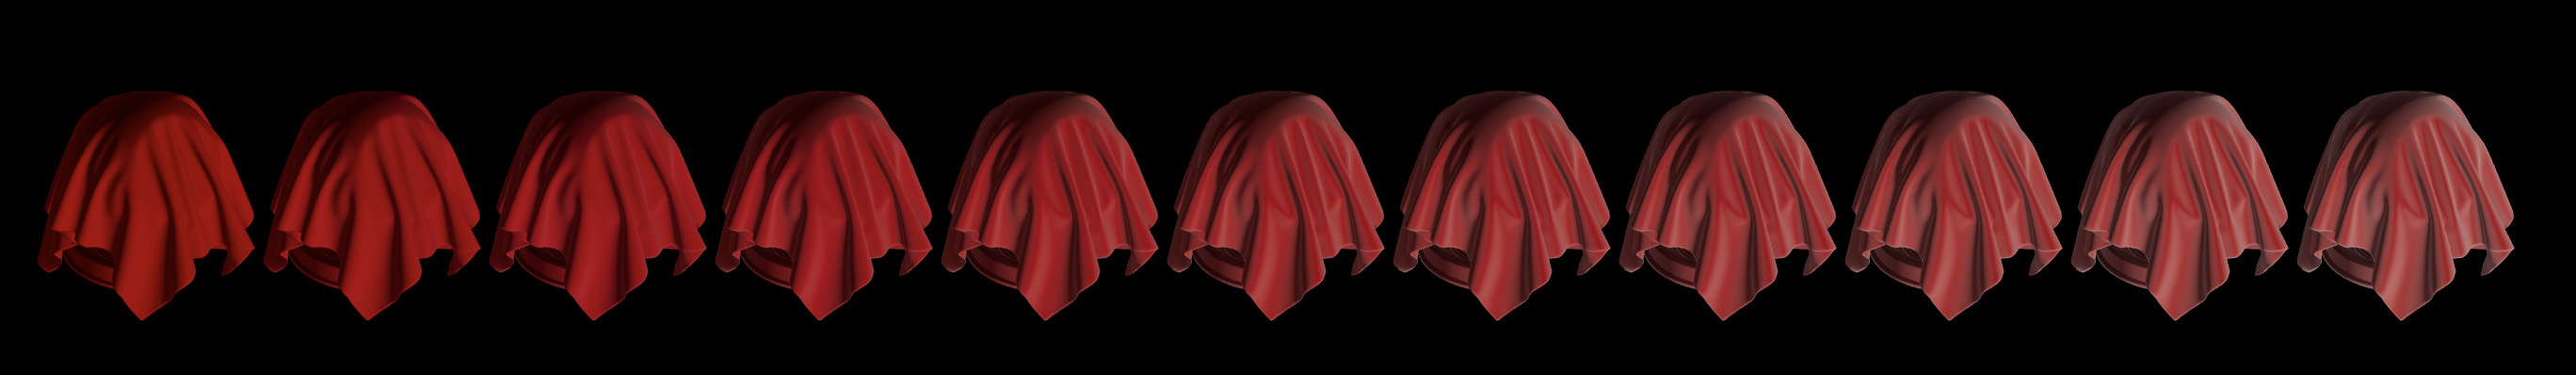
\includegraphics[scale=0.3]{results/ok_sheenintensity.jpg}}
  \caption{Interpolaci\'on de un color de \textit{sheen} aumentando su luminosidad frente a un color base constante.}
\end{figure}

El nuevo material no ofrece un control directo sobre la intensidad del \textit{sheen}, sin embargo, un efecto similar se puede
alcanzar utilizando un el mismo que el color base aumentando la luminosidad como se muestra en la figura 5.4.

\begin{figure}[H]
  \vspace{0.5cm}
  \centering
    \frame{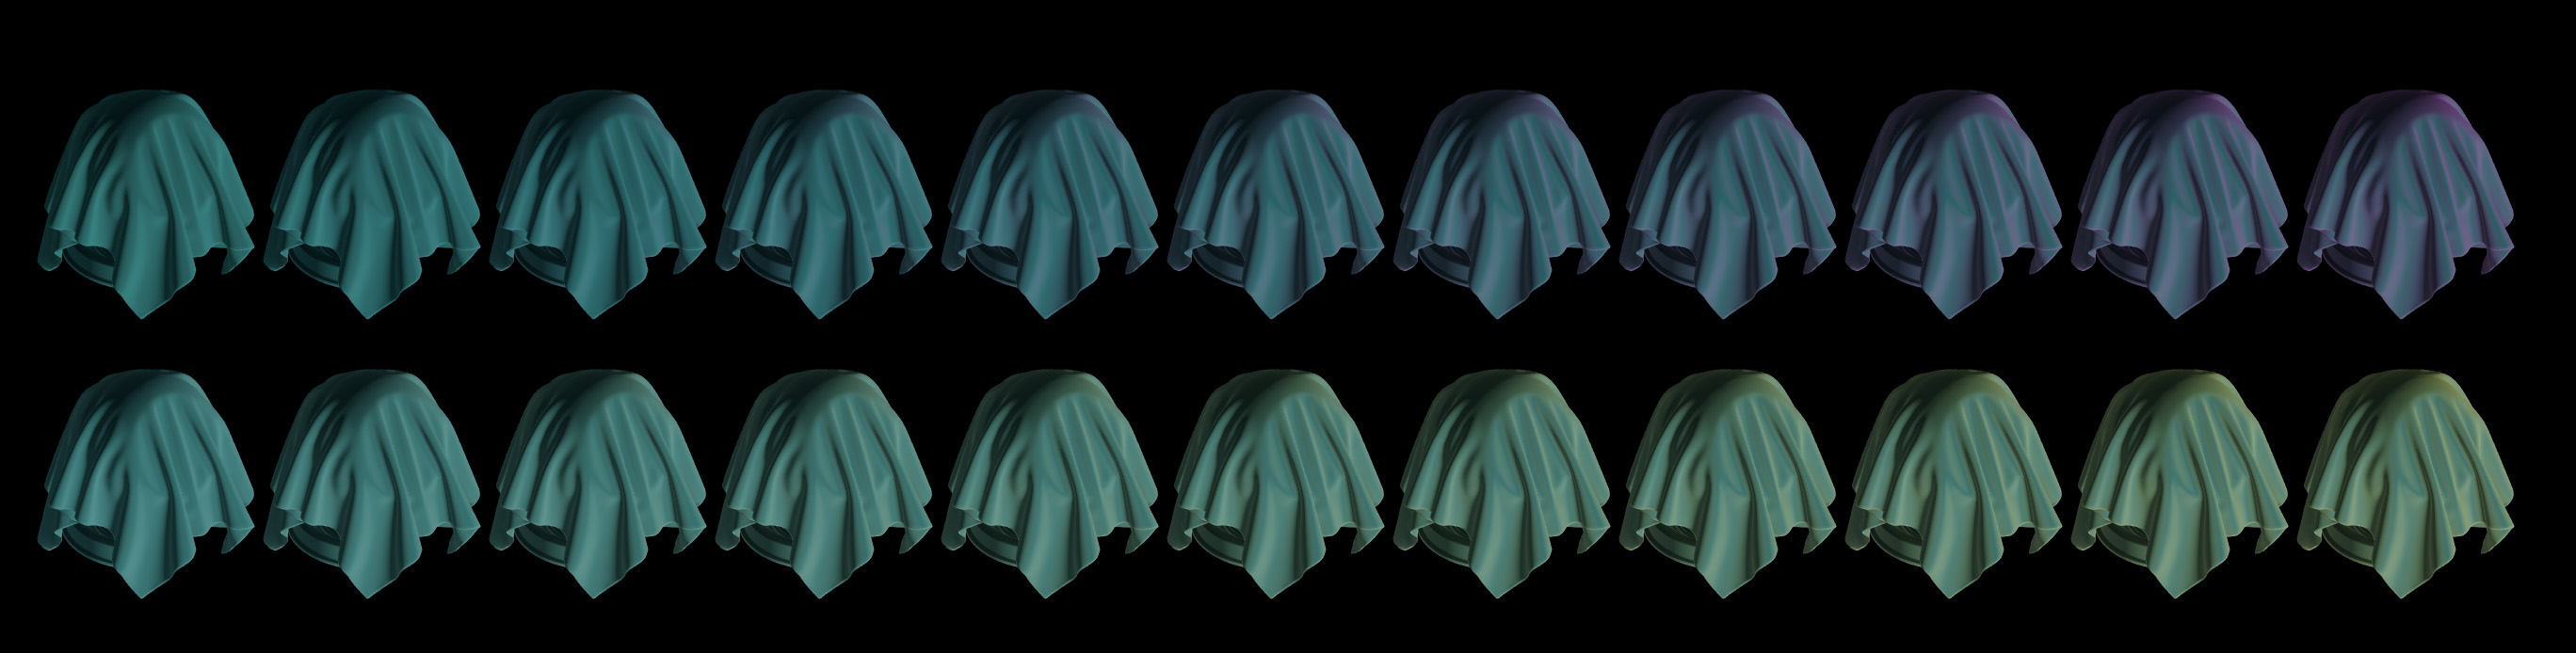
\includegraphics[scale=0.3]{results/ok_sheentint.jpg}}
  \caption{Interpolaci\'on de un color de \textit{sheen} aumentando su saturacion frente a un color base constante.}
\end{figure}
\singlespacing

Como se muestra en la figura 5.5, utilizar un color de \textit{sheen} diferente al color base permite conseguir reflexiones especulares
en dos tonos como resultado de la combinaci\'on del color base y el \textit{sheen}.

\begin{figure}[H]
  \vspace{0.5cm}
  \centering
    \frame{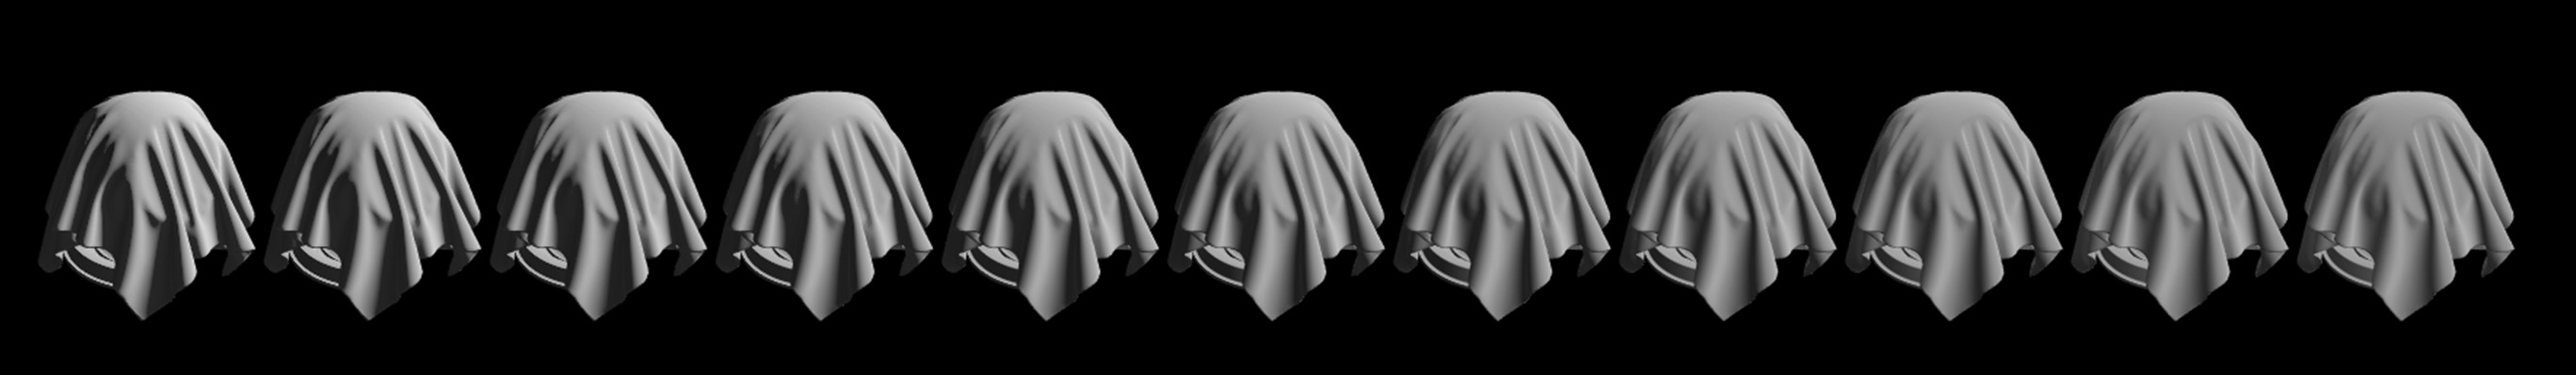
\includegraphics[scale=0.3]{results/ok_subsurfaceintensity.jpg}}
    \caption{Interpolaci\'on de \textit{subsurfaceIntensity} utilizando un color base y color de \textit{subsurface} blancos.}
\end{figure}
\singlespacing

En la figura 5.6, se utiliza el blanco como color base y \textit{subsurface}. La interpolaci\'on del par\'ametro de \textit{subsurfaceIntensity}
muestra una transici\'on de sombras m\'as intensas (\textit{subsurfaceIntensity = 0}) a sombras m\'as suaves, que toman el color base del
\textit{subsurface} (\textit{subsurfaceIntensity = 1})\\

% el color base permanece constante, mientras que el \textit{subsurface}, de un tono similar al color base,
% aumenta su saturaci\'on. Del mismo modo que en el \textit{sheen}, jugando con el valor de luminosidad del \textit{subsurface},
% se puede obtener control sobre la intensidad del efecto.


\begin{figure}[H]
  \vspace{0.5cm}
  \centering
    \frame{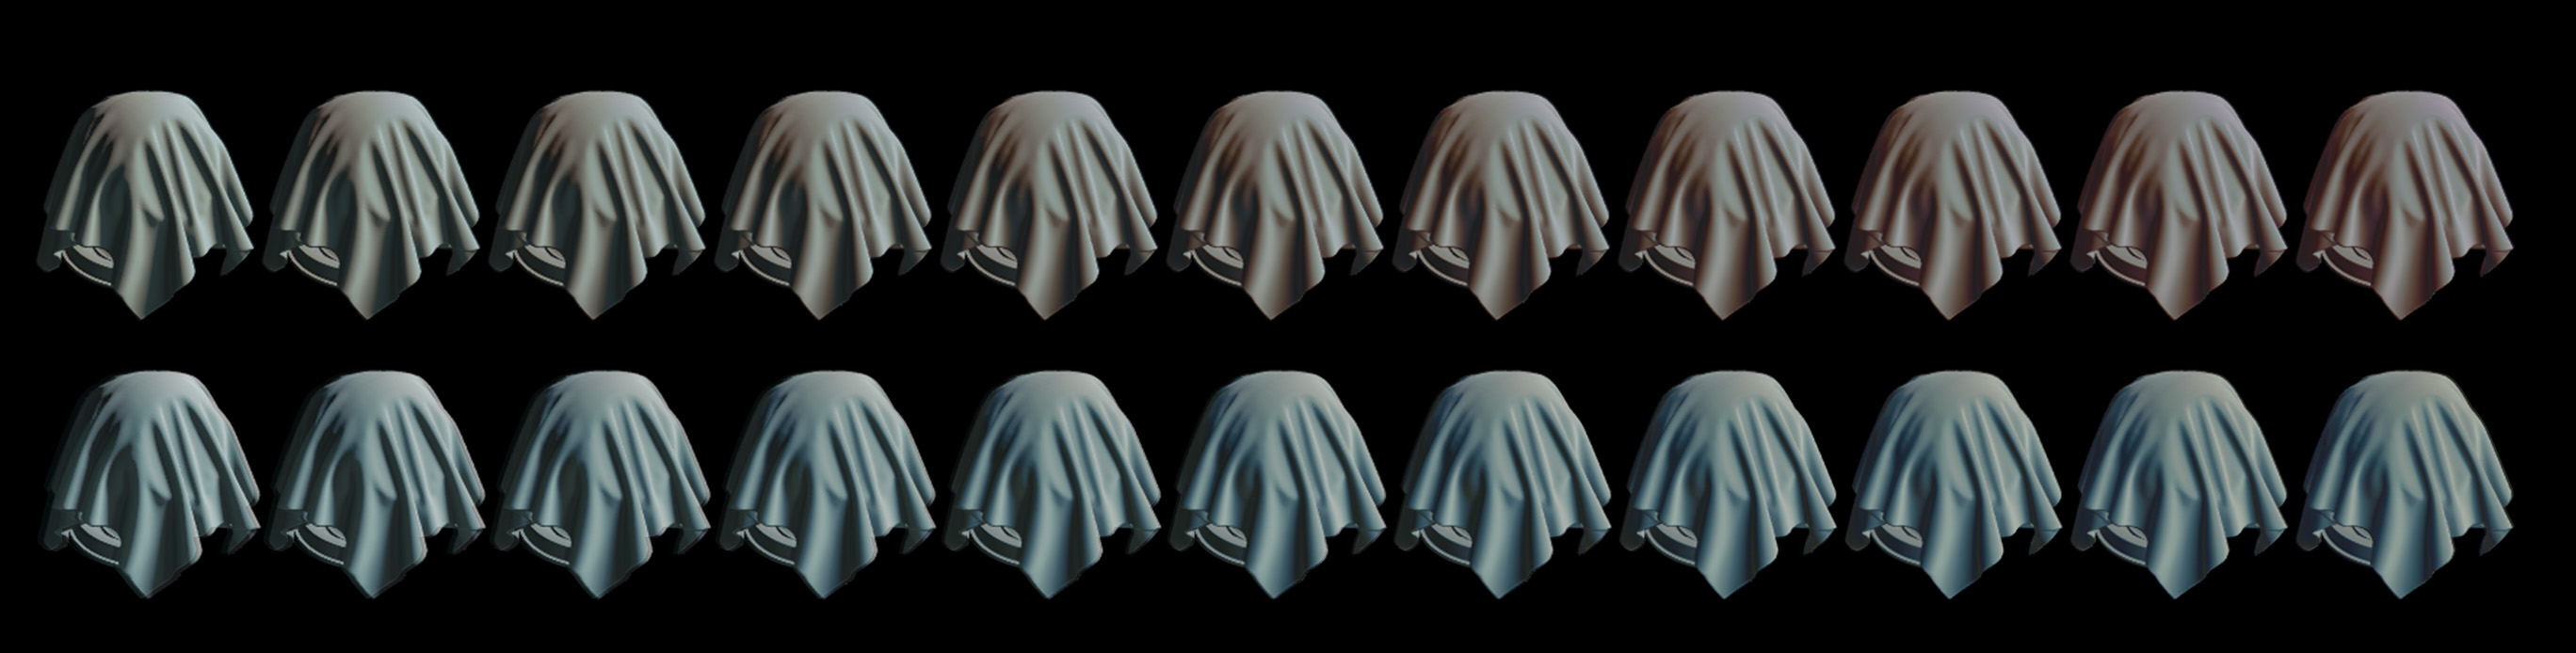
\includegraphics[scale=0.3]{results/ok_subsurfacetint.jpg}}
    \caption{Interpolaci\'on de un color de \textit{subsurface} frennte a un color base constante.}
 \end{figure}
\singlespacing

La figura 5.7 muestra interpolaciones entre un color base constante (blanco) y un color de \textit{subsurface},
rojo en la fila superior y azul en la fila inferior. Subiendo el valor de \textit{subsurfaceIntensity}
se puede apreciar como el tejido se ti\~ne progresivamente del color de \textit{subsurface}.

% se utilizan dos tonos de color complementarios para el color base y el \textit{subsurface}. El color
% base es constante, mientras que el \textit{sheen} aumenta por pasos su saturaci\'on.
% El factor de correcci\'on aplicado sobre el color difuso, que simula el efecto de reflexi\'on interna, ti\~ne progresivasivamente
% las sombras del color asignado al par\'ametro \textit{subsurface}.

% Las siguientes comparativas son matrices bidimensionales que muestran la evoluci\'on de un par\'ametro por cada uno de los ejes
% $x$ e $y$ y permiten ver la relaci\'on entre estos dos par\'ametros y su efecto sobre la apariencia final del material.\\

% En la comparativa de la figura 6.7, se muestra en el eje $x$ un aumento del efecto de \textit{sheen}, mientras que en el
% eje $y$ aumenta el valor de roughness del material. Se puede apreciar que con valores bajos de \textit{sheen}, el efecto
% se aprecia con intensidad en los \'angulos cr\'iticos y decae r\'apidamente, mientras que para valores altos de este par\'ametro,
% el efecto se extiende hacia los tonos medios, creando una transici\'on m\'as suave entre el color base y el de \textit{sheen}.\\

% La figura 6.8 muestra los incrementos del color de \textit{sheen} en el eje $x$ e incrementos en el eje $y$ del color de subsurface.
% El \textit{sheen} de color verde simula el efecto de retrodispersi\'on que ti\~ne el brillo especular de \'este color, mientras
% que el \textit{subsurface}, de color rojo, da a los tonos medios un color rojizo. El valor de \textit{roughness} del material
% es alto, es por ello que a medida que aumentan los valores de \textit{subsuface}, \textit{sheen}, se aprecia una transici\'on
% suave entre estos dos par\'ametros, que proporcionan el aspecto amarillo/anaranjado, como resultado de la transici\'on entre
% el verde del brillo especular y el rojo de las sombras y tonos medios.

\begin{figure}[H]
  \vspace{0.5cm}
  \centering
    \frame{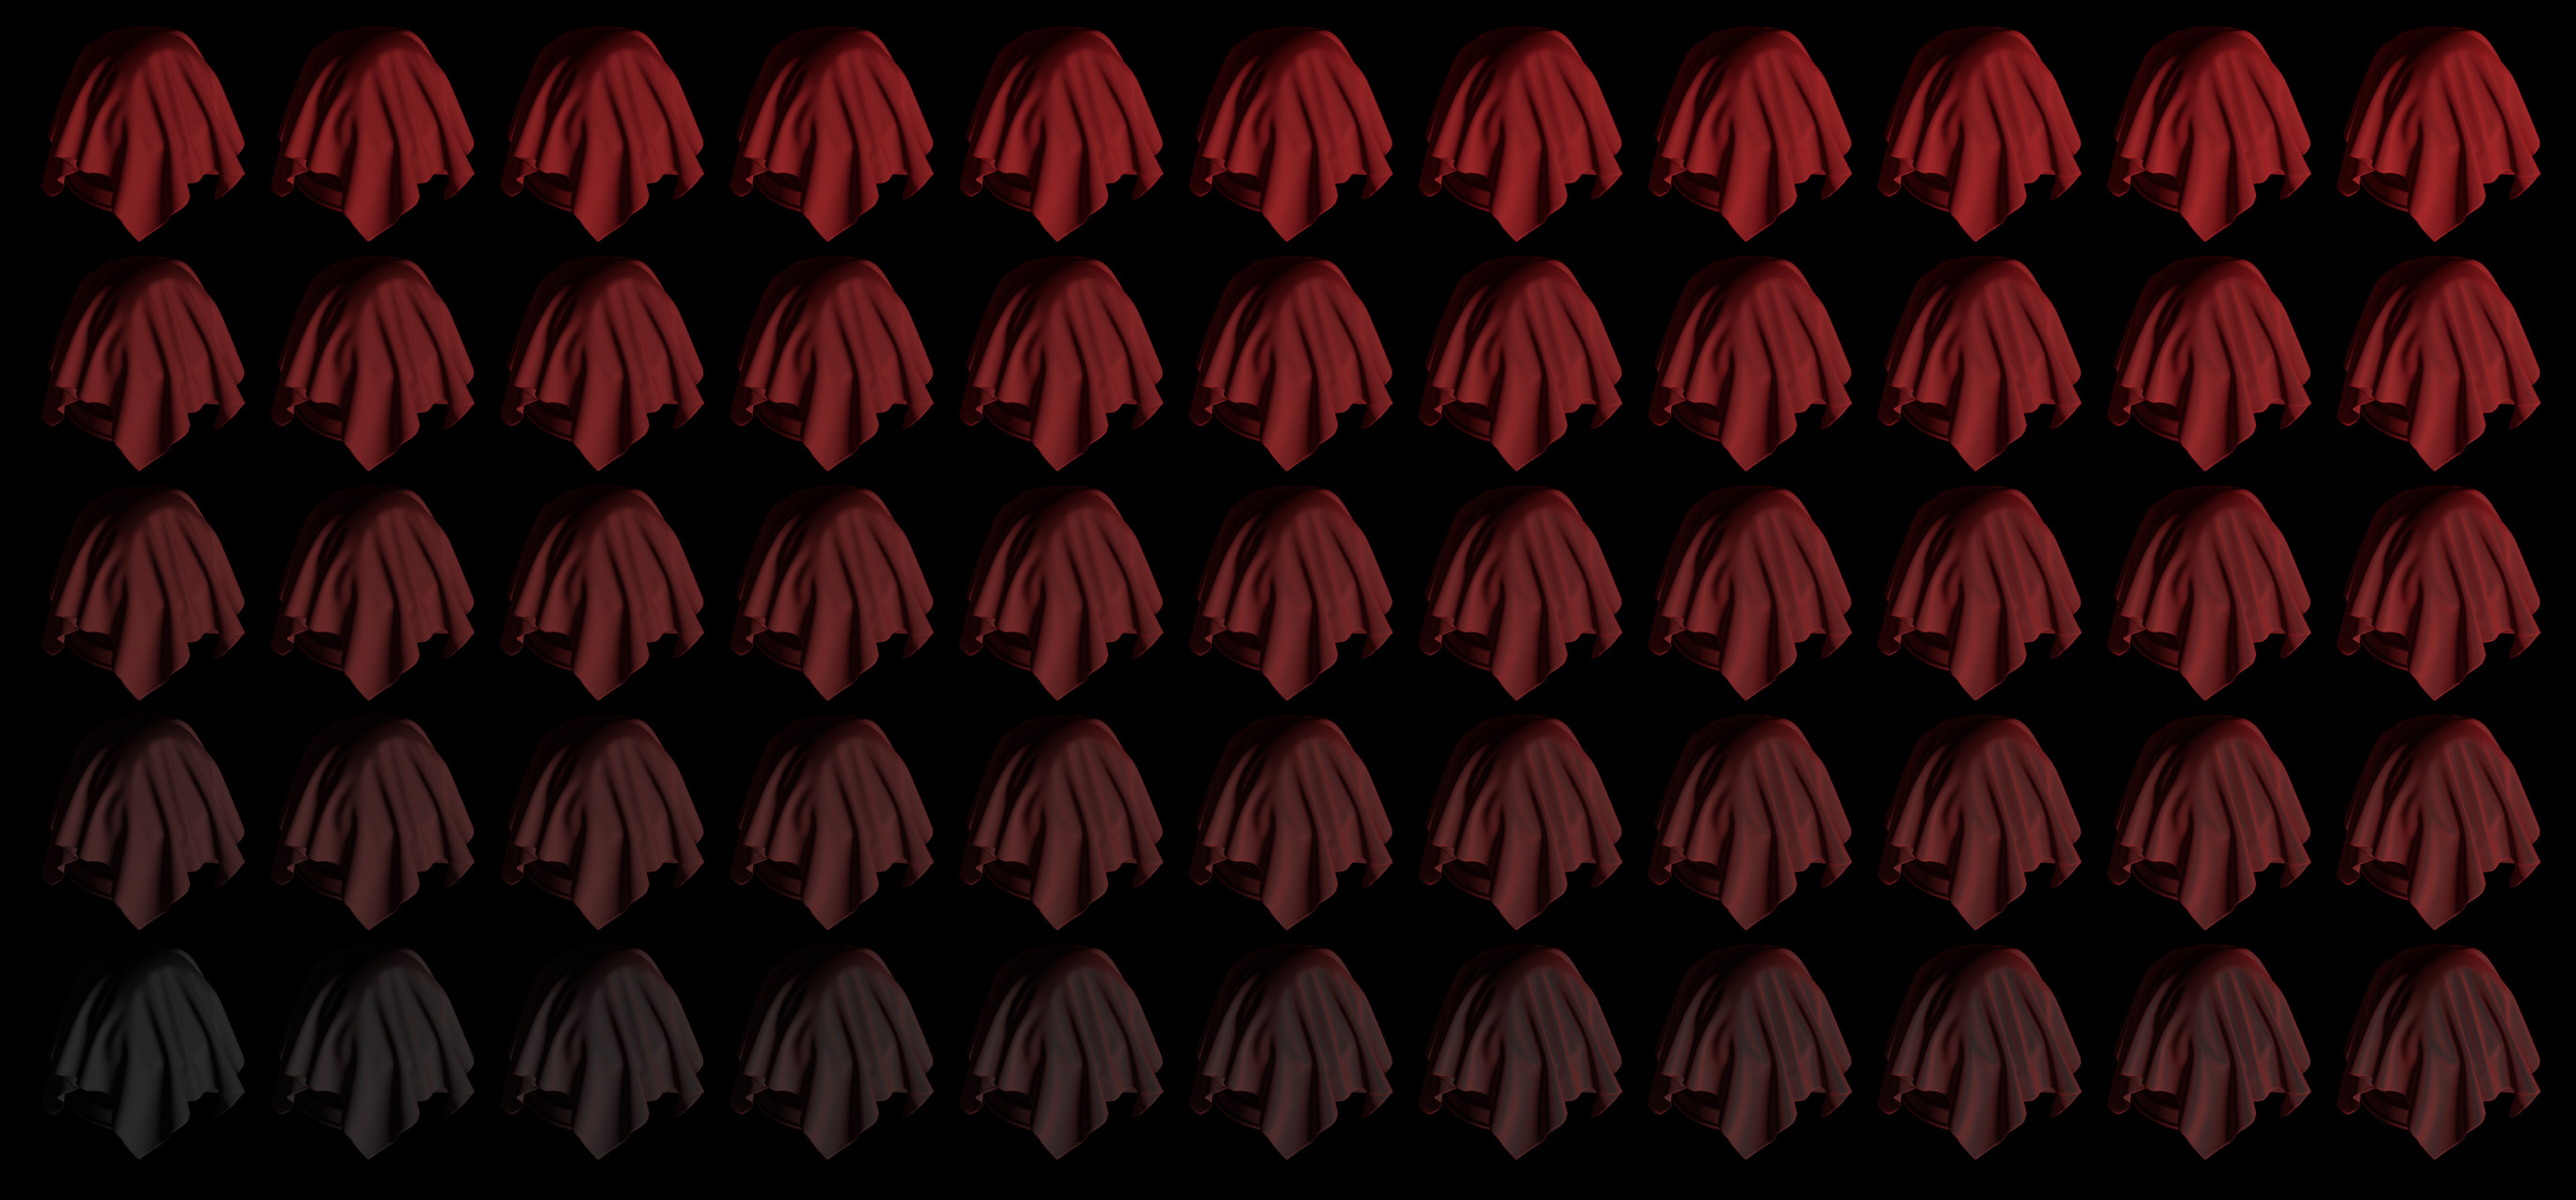
\includegraphics[scale=0.3]{results/ok_basecolorsheen.jpg}}
    \caption{Interpolaci\'on del color de sheen en el eje $x$ frente a interpolaci\'on del color base en el eje $y$.}
\end{figure}

La matriz bidimentsional de la figura 5.8 utiliza un color de sheen que se interpola entre el color base del tejido,
gris oscuro, hasta un rojo intenso en el eje $x$, mientras que en el eje $y$, el color base se interpola hacia el mismo
tono rojo que el \textit{sheen}.\\

\singlespacing
A continuaci\'on se muestran comparativas entre el \textit{MeshPhysicalMaterial} de ThreeJs, el nuevo \textit{MeshClothMaterial}
y las im\'agenes generadas por el motor de trazado de rayos.

\begin{figure}[H]
  \vspace{0.5cm}
  \centering
    \frame{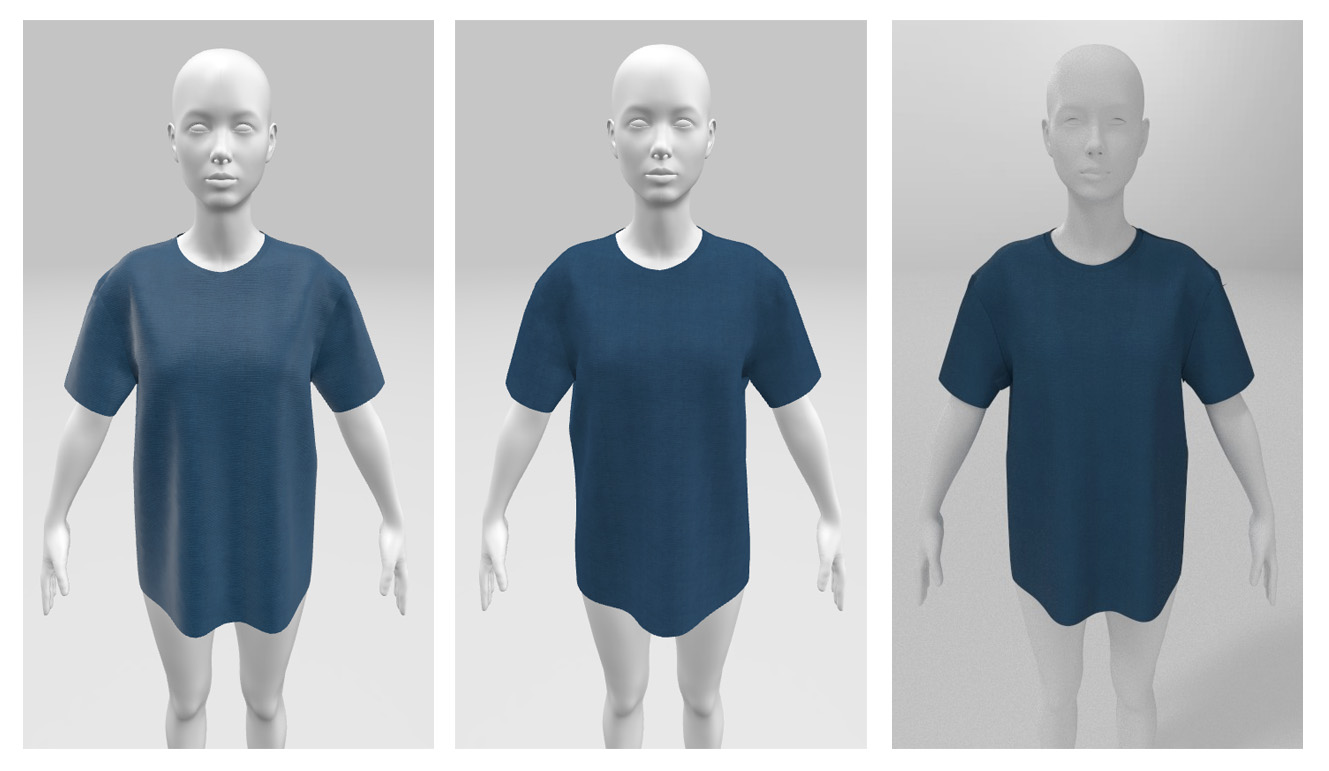
\includegraphics[scale=0.3]{results/lenda}}
    \caption{Tejido de canvas renderizado con \textit{MeshPhysicalMaterial}, \textit{MeshClothMaterial} y el servicio de renderizado de trazado de rayos de Seddi}
\end{figure}

Mientras que el brillo especular de \textit{MeshPhysicalMaterial} da al tejido un aspecto de pl\'astico, el mayor control sobre
el especular de \textit{MeshClothMaterial} permite atenuar el efecto consiguiendo una mayor coherencia con los resultados obtenidos
por el servicio de renderizado en la nube de Seddi.

\begin{figure}[H]
  \vspace{0.5cm}
  \centering
    \frame{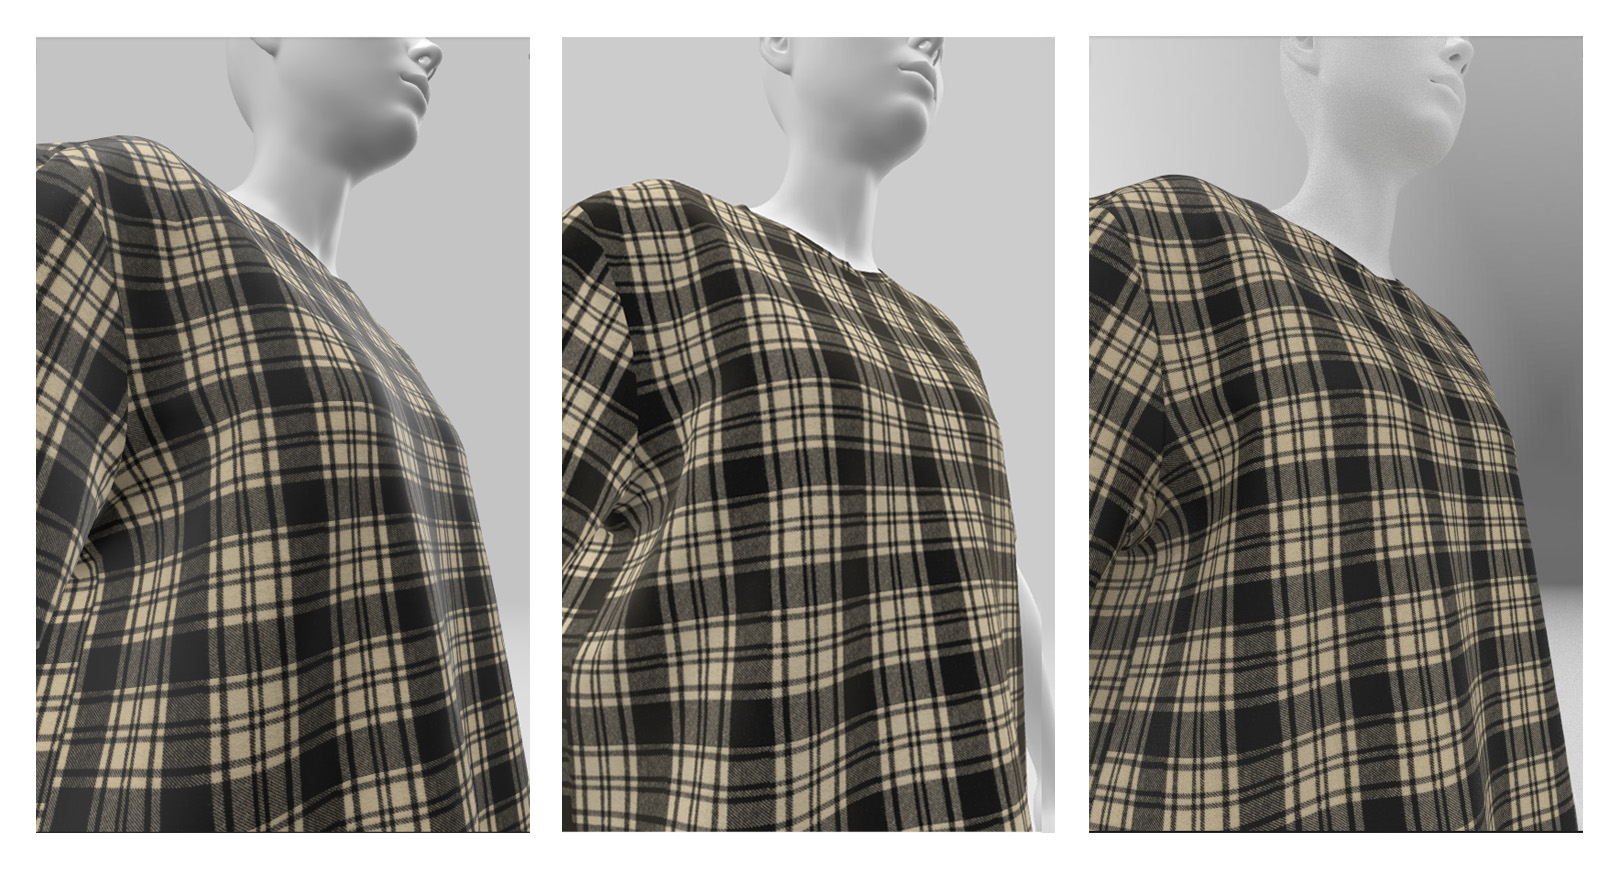
\includegraphics[scale=0.2458]{results/tartantwillbrushed}}
    \caption{Tejido de sarga renderizado con \textit{MeshPhysicalMaterial}, \textit{MeshClothMaterial} y el servicio de renderizado de trazado de rayos de Seddi}
\end{figure}

De igual forma, en la figura 5.10, se aprecia como el \textit{MeshPhysicalMaterial} falla al capturar un tejido de sarga, cuyas reflexiones
son muy definidas el \'angulo cr\'itico. Por su parte, el \textit{MeshPhysicalMaterial} utiliza un color marr\'on con
muy baja luminosidad que aten\'ua el efecto consiguiendo un resultado m\'as parecido al obtenido por el motor de trazado de rayos.

      \chapter{Resultados}
      \chapter{Discusi\'on y trabajo futuro}

    \appendix
      \addcontentsline{toc}{chapter}{Appendix}
      \chapter{Conceptos b\'asicos}

\section{Unidades b\'asicas radiom\'etricas}
\todo[inline]{Cambiar/completar}

\bgroup
    Cuando hablamos de la cantidad de luz, no es la medicion sobre un foton de luz independiente, si no que se tratan de medidas en relacion
    al tiempo, la direccion o el \'area.

    \begin{itemize}
    \item[] \textbf {{\'Angulo s\'olido}}
    \item[] \textbf {Flujo} La unidad que representa la energia sobre la unidad de tiempo es el flujo, representado por Phi. Es la energía que transportan las ondas
    por unidad de tiempo, se mide en vatios. En los motores de render se utiliza para expresar la cantidad total de energia emitida por un a fuente de luz.
    \begin{equation}
        \Phi_e = \dfrac{d{Q_e}}{dt}
    \end{equation}
    \item[] \textbf {Intensidad}
    \begin{equation}
        I = \dfrac{d\Phi}{d\omega}
    \end{equation} 
    \item[] \textbf {Irradiancia} La irradiancia, es la cantidad de energ\'ia por unidad de tiempo por unidad de superficie, o flujo por superficie. Se representa como
    E, su unidad son los vatios/m2 y se utiliza para medir la cantidad de luz que incide sobre una superficie.
    \begin{equation}
        E = \dfrac{d\Phi}{dA}
    \end{equation}
    Cuando este flujo de radiancia se mide en direcci\'on contraria, de salida, se llama emitancia (M)
    \item[] \textbf {Radiancia} Simula luz tan lejana que sus rayos son paralelos entre si, como por ejemplo el sol.
    \begin{equation}
        L = \dfrac{d^2\Phi}{dA_{proj}d\omega}
    \end{equation}
    \end{itemize}
\egroup

\section{BxDF}
    \bgroup
    A continuaci\'on se detallan los nombres de las funciones en funcion del fen\'omeno f\'isico que modelan.
    \begin{itemize}
        \item[] \textbf {BRDF} Es la funci\'on que modela el comportamiento de la luz al golpear una superficie opaca, la reflexi\'on. Fue definido por primera vez en 1965 por
        Fred Nicodemus y su definici\'on es el ratio entre radiancia reflectada e irraciancia incidente.
        Para determinar el \'angulo de salida del rayo se utiliza la ley de la reflexi\'on y las tres caracter\'isticas que ha de cumplir un BRDF basado en
        f\'isica es que sea positivo, que cumpla con la reciprocidad de Helmholtz y que cumpla con la ley de conservaci\'on de la energ\'ia.
        \item[] \textbf {BTDF} Describe el comportamiento del rayo de luz al atravesar una superficie, la refracci\'on. Para calcular el angulo de salida del rayo se utiliza la
        ley de Snell, y al contrario que el BRDF, no sumple el principio de reciprocidad de Helmholtz.
        \item[] \textbf {BSSRDF y BSSTF} Son ampliaciones del modelo de reflexi\'on y refracci\'on, respectivamente, teniendo en cuenta las reflexiones internas del rayo a traves de la
        superficie del objeto.
        \item[] \textbf {BSDF} Se utiliza comunmente para hablar de cualquier forma de BxDF. En un sentido mas estricto, se refiere al conjunto de un BSSRDF y un BSSTDF.
    \end{itemize}
    \egroup

    \section{Integraci\'on con ThreeJs}
    La soluci\'on elegida para extender el sistema de materiales de Three ha sido crear un fork, extendiendo la
    librer\'ia para implementar las funcionalidades necesarias que dan soporte a estos nuevos motores de shading.
    Siguiendo la nomenclatura, de ThreeJs (MeshStandardMaterial, MeshPhysicalMaterial, etc) se ha creado un material
    MeshClothMaterial, basado en los material Cloth de Filament.\\
    ThreeJs utiliza un sistema de chunks (trozos) se componen en tiempo de ejecuci\'on para acabar formando los vertex
    y fragment shaders que se utilizan en los programas de WebGL. Los chunks se componen en la libreria de shaders, la
    clase ShaderLib.
    Para crear nuestro MeshClothMaterial, hemos de extender de la clase base Material, de la que extienden el resto de
    materiales. En este caso, de la misma forma que hace MeshPhysicalMaterial, extenderemos de MeshStandardMaterial,
    que dispone de la mayor parte de uniforms y attributes que necesita nuestro shader.\\

    \bgroup

    \begin{lstlisting}[caption=Clase MeshClothMaterial]
import { Vector2 } from '../math/Vector2.js';
import { MeshStandardMaterial } from './MeshStandardMaterial.js';
import { Color } from '../math/Color.js';
import brdfCloth from './clothBRDF.js';

/**
    * parameters = {
    *  reflectivity: <float>,
    *
    *  sheen: <Color>,
    *
    *  transmission: <float>,
    *  transmissionMap: new THREE.Texture( <Image> ),
    *
    *  subsurface: <Vector3>,
    * }
    */

function MeshClothMaterial( parameters ) {

    MeshStandardMaterial.call( this );

    this.defines = {

    'STANDARD': '',
    'CLOTH': ''

    };

    this.type = 'MeshClothMaterial';
    this.sheen = null;

    this.transmission = 0.0;
    this.transmissionMap = null;
    this.subsurface = null;

    this.brdfCloth = brdfCloth;

    this.setValues( parameters );

}

MeshClothMaterial.prototype = Object.create( MeshStandardMaterial.prototype );
MeshClothMaterial.prototype.constructor = MeshClothMaterial;

MeshClothMaterial.prototype.isMeshClothMaterial = true;

MeshClothMaterial.prototype.copy = function ( source ) {

    MeshStandardMaterial.prototype.copy.call( this, source );

    this.defines = {

    'STANDARD': '',
    'CLOTH': ''

    };

    if ( source.sheen ) {

    this.sheen = ( this.sheen || new Color() ).copy( source.sheen );

    }

    this.transmission = source.transmission;
    this.transmissionMap = source.transmissionMap;

    if ( source.subsurface ) {

    this.subsurface = ( this.subsurface || new Color() ).copy( source.subsurface );

    } else {

    this.subsurface = null;

    }

    if ( source.brdfCloth ) {

    this.brdfCloth = source.brdfCloth;

    } else {

    this.brdfCloth = null;

    }

    return this;

};

export { MeshClothMaterial };
        
    \end{lstlisting}
    
    Para que el motor de render de ThreeJs reconozca este nuevo material es necesario, a\~nadir
    su tipo (MeshClothMaterial) al mapa de ShaderIds para que el gestor de programas (WebGLPrograms)
    lo utilice para detectar obtener los uniforms y shaders necesarios para el material. Adem\'as
    los nuevos par\'ametros necesarios para el material se deben de incluir en el array
    parametersNames, de forma que el sistema de cacheo de programas de ThreeJs detecte estas
    nuevas propiedades.\newline
    
    \begin{lstlisting}[caption=Clase MeshClothMaterial]
function WebGLPrograms( renderer, cubemaps, extensions, capabilities, bindingStates, clipping ) {

// ...

const shaderIDs = {
    MeshDepthMaterial: 'depth',
    MeshDistanceMaterial: 'distanceRGBA',
    MeshNormalMaterial: 'normal',
    MeshBasicMaterial: 'basic',
    MeshLambertMaterial: 'lambert',
    MeshPhongMaterial: 'phong',
    MeshToonMaterial: 'toon',
    MeshStandardMaterial: 'physical',
    MeshPhysicalMaterial: 'physical',
    MeshClothMaterial: 'cloth',
    MeshMatcapMaterial: 'matcap',
    LineBasicMaterial: 'basic',
    LineDashedMaterial: 'dashed',
    PointsMaterial: 'points',
    ShadowMaterial: 'shadow',
    SpriteMaterial: 'sprite'
};

const parameterNames = [
    "precision", "isWebGL2", "supportsVertexTextures", "outputEncoding", "instancing", "instancingColor",
    "map", "mapEncoding", "matcap", "matcapEncoding", "envMap", "envMapMode", "envMapEncoding", "envMapCubeUV",
    "lightMap", "lightMapEncoding", "aoMap", "emissiveMap", "emissiveMapEncoding", "bumpMap", "normalMap", "objectSpaceNormalMap", "tangentSpaceNormalMap", "clearcoatMap", "clearcoatRoughnessMap", "clearcoatNormalMap", "displacementMap", "specularMap", "subsurface", "brdfCloth",
    "roughnessMap", "metalnessMap", "gradientMap",
    "alphaMap", "combine", "vertexColors", "vertexTangents", "vertexUvs", "uvsVertexOnly", "fog", "useFog", "fogExp2",
    "flatShading", "sizeAttenuation", "logarithmicDepthBuffer", "skinning",
    "maxBones", "useVertexTexture", "morphTargets", "morphNormals",
    "maxMorphTargets", "maxMorphNormals", "premultipliedAlpha",
    "numDirLights", "numPointLights", "numSpotLights", "numHemiLights", "numRectAreaLights",
    "numDirLightShadows", "numPointLightShadows", "numSpotLightShadows",
    "shadowMapEnabled", "shadowMapType", "toneMapping", 'physicallyCorrectLights',
    "alphaTest", "doubleSided", "flipSided", "numClippingPlanes", "numClipIntersection", "depthPacking", "dithering",
    "sheen", "transmissionMap"
];

// ...

function getParameters( material, lights, shadows, scene, object ) {

    const shaderID = shaderIDs[ material.type ];

    // ...

    let vertexShader, fragmentShader;

    if ( shaderID ) {

    const shader = ShaderLib[ shaderID ];

    vertexShader = shader.vertexShader;
    fragmentShader = shader.fragmentShader;

    }

    // ...

    const parameters = {

    shaderID: shaderID,

    vertexShader: vertexShader,
    fragmentShader: fragmentShader,

    sheen: !! material.sheen,

    subsurface: !! material.subsurface,

    brdfCloth: !! envMap && shaderID === 'MeshClothMaterial',
    // ...
    };

    // ...

    return parameters;
}
    \end{lstlisting}

    Finalmente, en el gestor de materiales de ThreeJs, necesitamos a\~nadir un nuevo m\'etodo
    que actualice los unfiroms del programa creado, de la misma forma que se hace con los
    materiales nativos de la librer\'ia.\newline
    
    \begin{lstlisting}[caption=Clase WebGLMaterials]
function refreshMaterialUniforms( uniforms, material, pixelRatio, height ) {

    // ...

    if ( material.isMeshStandardMaterial ) {

    refreshUniformsCommon( uniforms, material );

    if ( material.isMeshPhysicalMaterial ) {

        refreshUniformsPhysical( uniforms, material );

    } else if ( material.isMeshClothMaterial ) {

        refreshUniformsCloth( uniforms, material );

    } else {

        refreshUniformsStandard( uniforms, material );

    }

    }

    // ...

    function refreshUniformsCloth( uniforms, material, environment ) {

    refreshUniformsStandard( uniforms, material, environment );

    uniforms.reflectivity.value = material.reflectivity; // also part of uniforms common

    if ( material.sheen ) {

        uniforms.sheen.value.copy( material.sheen );

    } else {

        uniforms.sheen.value.copy( material.color );
        uniforms.sheen.value.r = Math.sqrt( uniforms.sheen.value.r );
        uniforms.sheen.value.g = Math.sqrt( uniforms.sheen.value.g );
        uniforms.sheen.value.b = Math.sqrt( uniforms.sheen.value.b );

    }

    if ( material.subsurface ) uniforms.subsurface.value.copy( material.subsurface );

    if ( material.brdfCloth ) uniforms.brdfCloth.value = material.brdfCloth;

}
        
    \end{lstlisting}

    De esta forma, tenemos un material con la interfaz nativa de ThreeJs, que tiene acceso a los
    chunks definidos en la clase ShaderChunk y cuyos uniforms y composici\'on de chunks definiremos
    en ShaderLib.\newline

    El BRDF para el componente especular de la iluminaci\'on directa del material Cloth de Filament,
    se utiliza en ThreeJs para a\~nadir opcionalmente un l\'obulo de Sheen al material. Por otra
    parte, el difuso, utiliza en Filament un t\'ermino opcional para ofrecer una aproximaci\'on
    barata el subsurface scattering para iluminaci\'on directa que utiliza Filament.\newline
    
    \begin{lstlisting}[caption=Implementaci\'on del BRDF de iluminaci\'on directa de Filament]
vec3 surfaceShading(const PixelParams pixel, const Light light) {
    vec3 h = normalize(shading_view + light.l);
    float NoL = light.NoL;
    float NoH = saturate(dot(shading_normal, h));
    float LoH = saturate(dot(light.l, h));

    // specular BRDF
    float D = D_Charlie(pixel.roughness, NoH);
    float V = V_Neubelt(shading_NoV, NoL);
    vec3  F = pixel.f0; // f0 is sheen color for Cloth materials 
    vec3 Fr = (D * V) * F;

    // diffuse BRDF
    float diffuse = diffuse(pixel.roughness, shading_NoV, NoL, LoH);
    #if defined(MATERIAL_HAS_SUBSURFACE_COLOR)
    diffuse *= Fd_Wrap(dot(shading_normal, light.l), 0.5);
    #endif

    vec3 Fd = diffuse * pixel.diffuseColor;

#if defined(MATERIAL_HAS_SUBSURFACE_COLOR)
    Fd *= saturate(pixel.subsurfaceColor + NoL);
    vec3 color = ( Fd + Fr * NoL ) * light.colorIntensity
#else
    vec3 color = Fd + Fr * NoL * light.colorIntensity;
#endif

    return color;
}
    \end{lstlisting}
    
    Primero definimos la interfaz de nuestro MeshClothMaterial y pondremos en comparaci\'on con
    el MeshPhysicalMaterial, para analizar los par\'ametros en com\'un y los cambios en sus BRDF
    y ecuaciones de render.\newline
    
    \centering
    \begin{tabular}{| c | c |}
    \hline
    MeshPhysicalMaterial & MeshClothMaterial \\ \hline
    color & color \\
    roughness & roughness \\
    clearCoat & NO \\
    clearCoatRoughness & NO \\
    sheen  & sheen  \\
    NO  & subsurface  \\
    metalness & NO \\
    emissive & emissive \\
    alpha & alpha \\
    lightmap & lightmap \\
    normalMap & normalMap \\ \hline
    \end{tabular}\\
    \egroup
    \printbibliography
\end{document}